\documentclass[a4paper,11pt]{book}
\usepackage{listings}
\usepackage[utf8]{inputenc}
\usepackage{titlesec}
\usepackage{fancyhdr}
\usepackage[spanish,es-tabla]{babel}
\usepackage[hidelinks]{hyperref}
\usepackage{xcolor}
\usepackage{pdfpages}
\usepackage{eurosym}
\usepackage{graphicx}
\usepackage{caption}
\usepackage{subcaption}

% Información reutilizable
\newcommand{\asunto}{Trabajo de Fin de Grado}
\newcommand{\titulo}{Observatorio Remoto: un cliente INDI para Android}
\newcommand{\tituloEng}{Remote Observatory: A INDI client to Android}
\newcommand{\grado}{Grado en Ingeniería Informática}
\newcommand{\autor}{Jaime Torres Benavente}
\newcommand{\email}{jtbenavente@gmail.com}
\newcommand{\tutor}{Dr. Sergio Alonso Burgos}
\newcommand{\escuela}{Escuela Técnica Superior de Ingenierías Informática y de Telecomunicación}
\newcommand{\universidad}{Universidad de Granada}
\newcommand{\ciudad}{Granada}
\newcommand{\vers}{Versión 1.0}

% Información archivo
\hypersetup{
	pdfauthor = {\autor\ (\email)},
	pdftitle = {\titulo},
	pdfsubject = {\asunto},
	pdfkeywords = {móvil, android, atronomía, hardware astronómico, control,INDI, software libre},
	pdfcreator = {LaTeX con el paquete texlive},
	pdfproducer = {pdflatex}
}

% Estilo de cabeceras
\pagestyle{fancy}
\fancyhf{}
\fancyhead[LO]{\leftmark}
\fancyhead[RE]{\rightmark}
\fancyhead[RO,LE]{\textbf{\thepage}}
\setlength{\headheight}{1.5\headheight}

% Redefinición de comandos
\renewcommand{\lstlistingname}{Fragmento de código}
\renewcommand{\lstlistlistingname}{Índice de fragmentos de código}
\renewcommand{\chaptermark}[1]{\markboth{\textbf{#1}}{}}
\renewcommand{\sectionmark}[1]{\markright{\textbf{\thesection. #1}}}

% Definición de colores
\definecolor{gray97}{gray}{.97}
\definecolor{gray75}{gray}{.75}
\definecolor{gray45}{gray}{.45}
\definecolor{gray30}{gray}{.94}
\definecolor{lightgray}{rgb}{.9,.9,.9}
\definecolor{darkgray}{rgb}{.4,.4,.4}
\definecolor{purple}{rgb}{0.65, 0.12, 0.82}
\definecolor{background}{HTML}{EEEEEE}
\definecolor{delim}{RGB}{20,105,176}
\colorlet{punct}{red!60!black}
\colorlet{numb}{magenta!60!black}

% Listados
\lstset{
	aboveskip=0.5cm,
	backgroundcolor=\color{gray97},
	basicstyle=\scriptsize\ttfamily,
	breaklines=true,
	commentstyle=\color{gray45},
	frame=Ltb,
	framerule=0.5pt,
	framesep=0pt,
	framexbottommargin=3pt,
	framexleftmargin=0.1cm,
	framextopmargin=3pt,
	keywordstyle=\bfseries,
	numberfirstline = false,
	numbers=left,
	numbersep=6pt,
	numberstyle=\tiny,
	rulesep=.4pt,
	rulesepcolor=\color{black},
	showstringspaces = false,
	stringstyle=\ttfamily,
	literate={á}{{\'a}}1
	         {é}{{\'e}}1
	         {í}{{\'i}}1
	         {ó}{{\'o}}1
	         {ú}{{\'u}}1
	         {ñ}{{\~n}}1
}
 
% Minimizar fragmentado de listados
\lstnewenvironment{listing}[1][]
	{\lstset{#1}\pagebreak[0]}{\pagebreak[0]}

% Listado definido para JavaScript
% http://tex.stackexchange.com/questions/89574/language-option-supported-in-listings/89576#89576
\lstdefinelanguage{javascript}{
	backgroundcolor=\color{background},
	basicstyle=\footnotesize,
	breaklines=true,
	captionpos=b,
	comment=[l]{//},
	commentstyle=\color{purple}\ttfamily,
	frame=lines,
	identifierstyle=\color{black},
	keywordstyle=\color{blue}\bfseries,
	morecomment=[s]{/*}{*/},
	morestring=[b]',
	morestring=[b]",
	ndkeywordstyle=\color{darkgray}\bfseries,
	numbers=left,
	numbersep=8pt,
	numberstyle=\scriptsize,
	sensitive=false,
	showstringspaces=false,
	stepnumber=1,
	stringstyle=\color{red}\ttfamily,
	keywords={
		break,
		case,
		catch,
		catch,
		do,
		else,
		false,
		function,
		if,
		in,
		new,
		null,
		return,
		switch,
		true,
		typeof,
		var,
		while},
	ndkeywords={
		boolean,
		class,
		export,
		implements,
		import,
		this,
		throw}
}

% Listado definido para JSON
% http://tex.stackexchange.com/questions/83085/how-to-improve-listings-display-of-json-files/83100#83100
\lstdefinelanguage{json}{
	backgroundcolor=\color{background},
	basicstyle=\footnotesize,
	breaklines=true,
	captionpos=b,
	frame=lines,
	numbers=left,
	numbersep=8pt,
	numberstyle=\scriptsize,
	showstringspaces=false,
	stepnumber=1,
	literate=
		*{:}{{{\color{punct}{:}}}}{1}
		{,}{{{\color{punct}{,}}}}{1}
	    {\{}{{{\color{delim}{\{}}}}{1}
	    {\}}{{{\color{delim}{\}}}}}{1}
	    {[}{{{\color{delim}{[}}}}{1}
	    {]}{{{\color{delim}{]}}}}{1}
	    {ñ}{{\~{n}}}{1}
}

% Para que las páginas en blanco no tengan cabecera
\makeatletter
\def\clearpage{%
  \ifvmode
    \ifnum \@dbltopnum =\m@ne
      \ifdim \pagetotal <\topskip
        \hbox{}
      \fi
    \fi
  \fi
  \newpage
  \thispagestyle{empty}
  \write\m@ne{}
  \vbox{}
  \penalty -\@Mi
}
\makeatother

\begin{document}
\begin{titlepage}

\newlength{\centeroffset}
\setlength{\centeroffset}{-0.5\oddsidemargin}
\addtolength{\centeroffset}{0.5\evensidemargin}

\noindent\hspace*{\centeroffset}\begin{minipage}{\textwidth}

\centering

\includegraphics[width=0.9\textwidth]{../images/logo_ugr.png}\\[1.4cm]

\textsc{\Large\asunto\\[0.2cm]}
\textsc{\grado}\\[1cm]

{\Huge\bfseries \titulo\\}
\noindent\rule[-1ex]{\textwidth}{3pt}\\[3.5ex]
\end{minipage}

\vspace{2cm}
\noindent\hspace*{\centeroffset}\begin{minipage}{\textwidth}
\centering

\textbf{Autor}\\ {\autor}\\[2.5ex]
\textbf{Tutor}\\ {\tutor}\\[2cm]

\includegraphics[width=0.3\textwidth]{../images/logo_etsiit.png}\\[0.1cm]
\textsc{\escuela}\\
\textsc{---}\\
\ciudad, \today\\

\includegraphics[width=0.3\textwidth]{../images/CC-SA-logo.png}
\end{minipage}
\end{titlepage}
\frontmatter
\begin{center}
{\LARGE\bfseries\titulo}\\
\end{center}
\begin{center}
\autor\
\end{center}

\newpage
\thispagestyle{empty}
\
\vspace{3cm}

\noindent\rule[-1ex]{\textwidth}{2pt}\\[4.5ex]

Yo, \textbf{\autor}, alumno de la titulación \textbf{\grado} de la \textbf{\escuela\ de la \universidad}, autorizo la ubicación de la siguiente copia de mi Trabajo Fin de Grado (\textit{\titulo}) en la biblioteca del centro para que pueda ser consultada por las personas que lo deseen.

\bigskip
Además, este mismo trabajo es realizado bajo licencia \textbf{Creative Commons Attribution-ShareAlike 4.0} (\url{https://creativecommons.org/licenses/by-sa/4.0/}), dando permiso para copiarlo y redistribuirlo en cualquier medio o formato, también de adaptarlo de la forma que se quiera, pero todo esto siempre y cuando se reconozca la autoría y se distribuya con la misma licencia que el trabajo original. El documento en formato {\tt LaTeX} así como el código del proyecto se puede encontrar en el siguiente repositorio de {\tt GitHub}: \url{https://github.com/torresj/indi-android-ui}.

\vspace{4cm}

\noindent Fdo: \autor

\vspace{2cm}

\begin{flushright}
\ciudad, a \today
\end{flushright}

\newpage
\thispagestyle{empty}
\
\vspace{3cm}

\noindent\rule[-1ex]{\textwidth}{2pt}\\[4.5ex]

D. \textbf{\tutor}, profesor del \textbf{Departamento de Lenguajes y Sistemas Informáticos} de la \textbf{\universidad}.

\vspace{0.5cm}

\vspace{0.5cm}

\textbf{Informa:}

\vspace{0.5cm}

Que el presente trabajo, titulado \textit{\textbf{\titulo}}, ha sido realizado bajo su supervisión por \textbf{\autor}, y 
autoriza la defensa de dicho trabajo ante el tribunal que corresponda.

\vspace{0.5cm}

Y para que conste, expide y firma el presente informe en \ciudad\ a \today.

\vspace{1cm}

\textbf{El tutor:}

\vspace{5cm}

\noindent \textbf{\tutor}

\chapter*{Agradecimientos}
\thispagestyle{empty}

\vspace{1cm}

A mi familia porque gracias a ellos soy como soy.

\bigskip
A mis amigos porque sin ellos no habría podido llegar hasta aquí

\bigskip
A mi tutor \textbf{\tutor}, por aguantarme durante tantos meses con una paciencia infinita.


\begingroup
\let\cleardoublepage\clearpage
  \tableofcontents
  \listoffigures
  \listoftables
  \lstlistoflistings
\endgroup

\newpage
\thispagestyle{empty}
\
\mainmatter
\chapter{Resumen}

\section{Breve resumen y palabras clave}
\noindent{\textbf{Palabras clave}: \textit{móvil}, \textit{android}, \textit{astronomía}, \textit{hardware astronómico}, \textit{control}, \textit{INDI}, \textit{software libre}.\\

\bigskip
El objetivo principal de este proyecto es crear una aplicación móvil para controlar y monitorizar diferentes dispositivos astronómicos. 

\bigskip
Los avances tecnológicos de la última década han provocado la aparición de un hardware cada vez más sofisticado para usar en las actividades astronómicas. Todo esto unido al desarrollo de los dispositivos móviles y la conectividad a través de internet, han abierto un amplio abanico de posibilidades en un sector que busca la estandarización para permitir controlar cualquier dispositivo remotamente y que sea independiente del hardware concreto.

\bigskip
Actualmente podemos encontrar esfuerzos por implantar estándares para el control de dispositivos astronómicos. Uno de ellos es ASCOM\cite{SFA}, desarrollado bajo la plataforma \textit{Windows} y diseñado para controlar los dispositivos conectándolos a un ordenador. Para los objetivos de este proyecto, ASCOM no es una opción óptima ya que no está pensado para acceder remotamente, recurriendo a soluciones como el ``escritorio remoto'' de \textit{windows}.

\bigskip
Sin embargo existen soluciones de código abierto y multiplataforma como \textbf{INDI}\cite{INDILIB}.

\bigskip
\textbf{INDI} consiste a su nivel más básico en un protocolo que permite el control, automatización, obtención de datos e intercambio de los mismos entre distintos dispositivos hardware y programas cliente. La idea subyacente en el protocolo INDI es desacoplar aspectos específicos del hardware que se controla de tal manera que cambios en el hardware no impliquen necesariamente cambios en el software (cosa que ocurre en sistemas más habituales donde el el frontend software está fuertemente acoplado con el backend hardware).

\bigskip
Por otro lado, el gran auge de las tecnologías móvil, y en concreto de la plataforma \textbf{Android}, enmarcan el proyecto en un contexto ideal para poder conseguir el principal objetivo del proyecto, \textbf{crear una aplicación móvil para el control de instrumental astronómico}.

\bigskip
Además de crear una aplicación útil y fácilmente usable, basándonos en la filosofía del software libre y de mejora del software a través de terceros, se ha diseñado parte de la aplicación específicamente para facilitar la incorporación de nuevas vistas para dispositivos y propiedades. Se han definido las vistas por defecto que son transparentes a los tipos de propiedades y a los tipos de dispositivos. No obstante, se permite que cualquier persona pueda añadir sus vistas personalizadas sin tener que conocer como está diseñada e implementada toda la aplicación.

\bigskip
Por último, al ser un proyecto con muchas posibilidades, se considera que tiene un gran recorrido por lo que es un desarrollo vivo, que seguirá más allá del objetivo del presente documento y cuya finalidad es adaptarse de la forma más fiable posible a las necesidades reales de los astrónomos, ya sean amateurs o profesionales.

\newpage
\begin{center}
{\LARGE\bfseries\tituloEng}\\
\end{center}
\begin{center}
\autor\
\end{center}

\section{Extended abstract and key words}

\noindent{\textbf{Key words}: \textit{mobile}, \textit{android}, \textit{astronomy}, \textit{astronomical hardware}, \textit{control}, \textit{INDI}, \textit{free software}.\\

\bigskip
The main goal of this project is to create a mobile app to control and monitor different astronomical devices (hardware).

\bigskip
The advances in technology in the last decades have allowed astronomers all around the world (both professionals and amateurs) to use more sophisticated hardware in their usual astronomy activities. Typical astronomical devices are electronic mounts, that allow to track stars following the exact apparent movement of the sky, CCD cameras, that allow to capture images, electronic focusers and domes, weather stations and so on. All those improvements have additionally been enhanced with the development in network technologies and particular, with the popularization of Internet: not only is now possible to plug all your astronomical devices to your computer, but you can also control them remotely. This fact is increasing the interest of many amateur astronomers that with a relatively low budget can afford to install a remote observatory. It is worth mentioning that since light pollution is a huge problem for astronomy, those remote observatories are often located quite far from the astronomers headquarters (even thousand of kilometers away, in different continents).

\bigskip
To date, there have been efforts to establish standards for the control and monitoring of astronomical devices. One of the most used is ASCOM. However, this standard presents several disadvantages:

\bigskip
It's a Windows only based solution.
Its design allows complete freedom for the driver writers to develop a particular user interface for their devices, in a quite deep relation with the operating system. This fact complicates the development of network solutions for the observatory, since those interfaces cannot usually be serialized to the client computer.
Encourages closed software.

\bigskip
To overcome those problems, astronomers using ASCOM usually rely on remote desktop software to  control their remote observatories.

\bigskip
However, there are other different approaches to control astronomical devices that allow to overcome some of those problems. One of those approaches is INDI, a library that is used to control astronomical devices following a client / server architecture. In this way, the astronomical devices are connected to a computer (INDI server) and the INDI clients that allow the user interaction can be in another different machine. Moreover, as the INDI drivers abstract the different devices as collections of properties (numerical, textual, switches, lights and BLOBs) it is relatively easy to construct generic clients to control any INDI device, even if the device didn't exist at the time of the writing of the client. Additionally, INDI specs are open and the core INDI libraries (and many utilities, including clients and servers) are free software.

\bigskip
It is also important to note that controlling hardware remotely can be quite challenging. Not only you do not have direct control over the hardware (you cannot “unplug” it), but the amount of information that you have from it can be rather limited. Moreover, as weather conditions may vary quite fast (and rain,snow, wind or even direct sunlight can be very dangerous for the observatory equipment), it is necessary to have as many control resources as possible in case of emergencies.

\bigskip
Therefore, having a mobile app to control the equipment may easy many tasks, specially when unexpected events occur (power outages, network failures, and so on). This is the main reason of developing this project, to be able to control and monitor all your astronomical devices anywhere, at any time.
\chapter{Introducción}

El presente proyecto constituye un esfuerzo por unir las tecnologías móviles con la astronomía y los instrumentos astronómicos. En los siguientes apartados describiremos las distintas tecnologías o campos de estudio que se verán implicados en el desarrollo posterior:

\begin{itemize}
  \item \itembf{La astronomía.}
  \item \itembf{Instrumental astronómico.}
  \item \itembf{Control de dispositivos astronómicos.}
  \item \itembf{INDI.}
  \item \itembf{Dispositivos móviles.}
\end{itemize}

\section{La Astronomía}

Desde el princpio de los tiempos, el ser humano ha mirado al cielo con incertidumbre, viéndolo como una fuente inagotable de interrogantes sin resolver. En casi todas las religiones antiguas existía la \textbf{``cosmogonía''} que intentaba explicar el origen del universo, ligando este a los elementos mitológicos, dando paso esta a la \textbf{``astronomía''}:

\begin{quote}``\textit{Ciencia que se ocupa del estudio de los cuerpos celestes del universo, incluidos los planetas y sus satélites, los cometas y meteoritos, las estrellas y la materia interestelar, los sistemas de materia oscura, estrellas, gas y polvo llamados galaxias y los cúmulos de galaxias; por lo que estudia sus movimientos y fenómenos ligados a ellos.}''
\newline(\url{https://es.wikipedia.org/wiki/Astronom%C3%ADa})
\end{quote}

\bigskip
 La Astronomía es probablemente la más antigua de las ciencias naturales originándose en la antiguedad en casi todas las culturas humanas. Sus orígenes se pierden en prácticas religiosas de la prehistoria cuyos vestigios se encuentran en numerosos sitios arqueológicos (como Stonehenge) e incorporados todavía en la astrología una disciplina entrelazada con la astronomía y no separada de ella completamente hasta el siglo XVIII en el mundo occidental. La astronomía antigua constituyó las bases del calendario y la medida de periodos temporales como la semana el mes o el año. Los astrónomos antiguos eran capaces de distinguir entre estrellas y planetas dado que las primeras permanecen fijas en sus posiciones relativas mientras que los planetas se mueven una cantidad apreciable de espacio a lo largo de periodos relativamente cortos ( Saturno el más lento de los planetas conocidos en la antigüedad describe un periodo orbital en 29 años). La Astronomía antigua culmina con el desarrollo ordenado del modelo heliocéntrico expuesto en las obras de \textit{Ptolomeo}. Previamente \textit{Aristarco de Samos} había medido las distancias de la Tierra a la Luna y al Sol afirmando como consecuencia de éstas que el Sol era el centro del Universo alrededor del cual giraban los demás planetas incluyendo la Tierra. Otros logros destacados de la época clásica de la astronomía fueron los conseguidos por \textit{Hiparco} quien realizó el primer catálogo estelar y propuso un sistema de clasificación estelar en 6 magnitudes basado en la luminosidad aparente de las diferentes estrellas. La Astronomía en la Europa medieval se produce un oscurantismo en todos los campos del conocimiento incluyendo la astronomía. Ésta permanece preservada en escasas copias de tratados antiguos de la astronomía griega y romana. La astronomía observacional tan sólo se conserva en el mundo árabe.

 \bigskip
 \textit{Tycho Brahe (1546-1601)} introdujo la idea de la precisión de la medida en astronomía e inventó y produjo una gran cantidad de instrumental astronómico previo al telescopio. \textit{Galileo Galilei (1564-1642)} construyó su propio telescopio a partir de un invento holandés y lo utilizó inmediatamente en el estudio astronómico descubriendo los cráteres de la Luna, las lunas de Júpiter y las manchas solares. Sus observaciones tan sólo eran compatibles con el modelo \textbf{copernicano}. Paralelamente \textit{Johannes Kepler} expuso sus famosas \textbf{leyes de Kepler} para el movimiento de los planetas basándo su trabajo en las detalladas observaciones de \textit{Tycho Brahe}.

\bigskip
Una generación más tarde Isaac Newton fue el primer científico que unió la Física con la Astronomía proponiendo que las mismas fuerzas que hacían caer los cuerpos sobre la Tierra causaban el movimiento de los planetas y la Luna. Utilizando su Ley de la gravedad las leyes de Kepler resultan inmediatamente explicadas. Newton también descubrió que la Luz blanca del Sol está descompuesta en diferentes colors, un hecho importantísimo para el futuro desarrollo de la astronomía.

\bigskip
La \textbf{astronomía} es una de las pocas ciencias en las que los aficionados aún puden desempeñar un papel activo, especialmente en el descubirmientos y seguimiento de fenómenos. Es por ello que existe una gran variedad de \textbf{herramientas} e \textbf{instrumental astronómico} que permiten a cualquier persona obervar el universo.

\newpage
\section{Instrumental Astronómico}

Existe una gran variedad de \textbf{instrumental astronómico} en la actualidad. A continuación se describen las familias más importantes.

\subsection{Telescopios}

\begin{quote}``\textit{El telescopio es un instrumento óptico que permite ver objetos lejanos con mucho más detalle que a simple vista al captar radiación electromagnética, tal como la luz.}''
\newline(\url{https://es.wikipedia.org/wiki/Telescopio})
\end{quote}

\begin{figure}[!ht]
  \begin{center}
  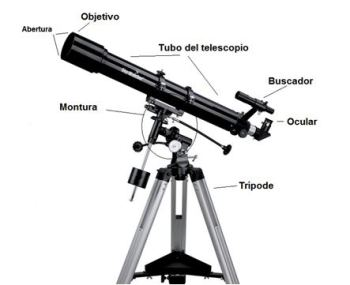
\includegraphics[width=1\textwidth]{../images/telescopio.jpg}
  \caption{Telescopio (\url{https://josevicentediaz.files.wordpress.com}).}
  \label{fig:diag_scrum}
  \end{center}
\end{figure}

\bigskip
Hace cuatro siglos nació un invento que habría de redefinir nuestro lugar en el universo. Tachado en su momento como el instrumento más diabólico de la historia, el telescopio sacudió la sociedad hasta las raíces. Al alzar los ojos al cielo nos convencimos de que éramos el centro de la creación, y había razones para ello: desde nuestra perspectiva, todo parece girar en torno a la Tierra

\bigskip
Los fabricantes de vidrio sabían desde la antigüedad que una esfera de vidrio podía aumentar imágenes, pero tuvieron que pasar siglos antes de que alguien ensamblara dos lentes en un tubo y mirara a través de ellas. Señalar la fecha, lugar y autor exactos de su invención es controvertido. Los holandeses se inclinan por el 2 de octubre de 1608, el día en que \textit{Hans Lippershey} patentó un instrumento llamado \textbf{kijker}, que significa mirador. Un moledor de vidrio holandés aseguraba haber inventado un aparato similar, pero el primero en patentarlo fue \textit{Lippershey}. Como era alemán, vivía en Holanda y registró la patente en Bélgica, más de un país ha pugnado por el honor de su autoría. Sin embargo, como dijo \textit{Darwin}:
\begin{quote}``\textit{en la ciencia el crédito es del que convence al mundo y no del primero en tener la idea}''
\newline(\textbf{Charles Darwin})
\end{quote}
Por eso la gloria se la llevó Italia, ya que fueron las mejoras que introdujo \textit{Galileo} las que permitieron usar el aparato como instrumento astronómico. El diseño de \textit{Galileo} consistía en una lente convexa para el objetivo y otra cóncava en el ocular. En 1611 el alemán \textit{Johannes Kepler} fue el primero en usar dos lentes convexas que enfocaban los rayos en un mismo punto. La configuración de \textit{Kepler} aún se usa en binoculares y cámaras fotográficas modernas y es la base del telescopio refractor.

\bigskip
Tras la muerte de \textit{Galileo}, fue \textit{Isaac Newton} quien nos dio una nueva imagen del universo que sobrevivió 250 años hasta la llegada de \textit{Albert Einstein}.

\begin{quote}``\textit{Si he logrado ver más lejos ha sido porque me he subido a hombros de gigantes}''
\newline(\textbf{Isaac Newton})
\end{quote}

Y así, sobre la herencia de \textit{Galileo}, \textit{Newton} inventó el \textbf{telescopio reflector}, que es la base de los actuales. La innovación consistía en usar espejos en lugar de lentes para enfocar la luz y formar imágenes. Entonces el universo se nos abrió en todo su esplendor.

\subsection{Cámaras CCD}

Un dispositivo de carga acoplada (en inglés \textbf{Charge-Coupled Device}, conocido también como \textbf{CCD}), es un circuito integrado que contiene un número determinado de condensadores enlazados o acoplados. Bajo el control de un circuito interno, cada condensador puede transferir su carga eléctrica a uno o a varios de los condensadores que estén a su lado en el circuito impreso.

\bigskip
\begin{figure}[!ht]
  \begin{center}
  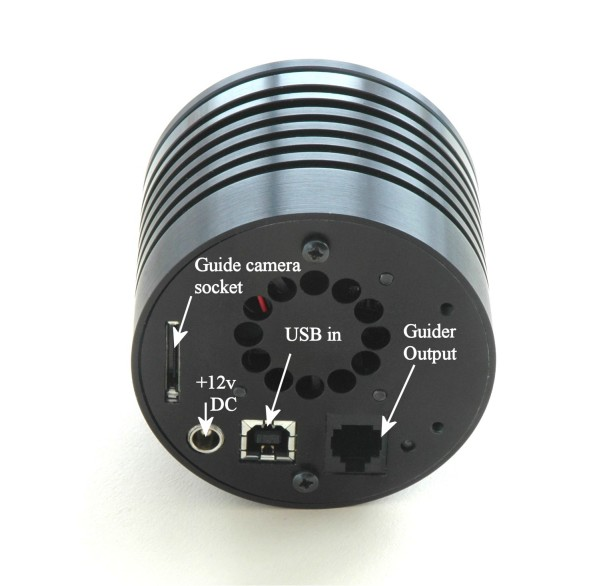
\includegraphics[width=1\textwidth]{../images/ccd.jpg}
  \caption{Cámara CCD (\url{http://www.lunatico.es/}).}
  \label{fig:diag_scrum}
  \end{center}
\end{figure}

\bigskip
El \textbf{CCD} se inventó a finales delos 60 por investigadores de \textbf{Bell Laboratories}. Originalmente se concibió como un nuevo tipo de memoria de ordenador pero pronto se observó que tenía muchas más aplicaciones potenciales tales como el proceso de señales y sobretodo la captación de imagen, esto último debido a la sensibilidad a la luz que presenta el silicio.

\bigskip
El sensor \textbf{CCD} de una cámara digital es como el motor de un coche, es la pieza principal. En su forma más elemental, el \textbf{CCD} es como un ojo electrónico que recoje la luz y la convierte en una señal eléctrica. Tienen dos diferencias básicas con los fotomultiplicadores:

\bigskip
Los sensores \textbf{CCD} son de menor tamaño y están construidos de semiconductores lo que permite la integración de millones de dispositivos sensibles en un solo chip.
La eficiencia cuóntica de los \textbf{CCD} (sensibilidad) es mayor para los rojos. Los fotomultiplicadores son más sensibles a los azules.

\bigskip
Físicamente, un \textbf{CCD} es una malla muy empaquetada de electrodos de polisilicio colocados sobre la superficie de un chip. Al impactar los fotones sobre el silicio se generan electrones generados que pueden guardarse temporalemte. Periódicamente se lee el contenido de cada pixel haciendo que los electrones se desplacen físicamente desde la posición donde se originaron (en la superficie del chip), hacia el amplificador de señal con lo que se genera una corriente eléctrica que será proporcional al número de fotones que llegaron al pixel. Para coordinar los periodos de almacenamiento (tiempo de exposición) y vaciado del pixel (lectura del pixel) debe existir una fuente eléctrica externa que marque el ritmo de almacenamiento-lectura: el reloj del sistema. La forma y amplitud de reloj son críticas en la operación de lectura del contenido de los pixeles.

\bigskip
Al tratarse el \textbf{CCD} de un dispositivo semiconductor, técnicamente es posible implementar en él todas las funciones electrónicas de un sistema de captación de imagen, pero esto no es rentable económicamente y por tanto se implementa en otros chips esternos al \textbf{CCD}: la mayoría de \textbf{CCD} de cámaras tienen varios chips (de tres a ocho).

\bigskip
La necesidad de usar chips distintos implica dos desventajas importantes; la necesidad de voltajes múltiples de abastecimiento de los chips y un gran consumo de potencia de todo el sistema electrónico.

\subsection{Monturas}

La montura de un telescopio es la parte mecánica que une el trípode o base al instrumento óptico. Existen varios tipos de monturas, algunas muy simples, otras mas complejas, incluso con correctores electrónicos y dispositivos de localización y seguimiento muy sofisticados (sistenas \textbf{GOTO})

\bigskip
\begin{figure}[!ht]
  \begin{center}
  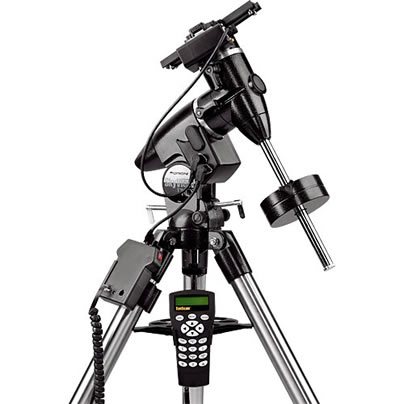
\includegraphics[width=1\textwidth]{../images/montura.jpg}
  \caption{Montura (\url{http://astrofacil.com/}).}
  \label{fig:diag_scrum}
  \end{center}
\end{figure}
http://nimax-img.de/

\bigskip
La montura tiene como objetivo proveer de movimiento controlado al telescopio. Es muy importante la firmeza y suavidad de los movimientos, para que la observación sea confortable y las astrofotografías perfectas. Las monturas se clasifican en dos grandes grupos, según los planos de referencia que utilicen (coordenadas).

\bigskip
La más simple es la montura altacimutal, que realiza movimientos horizontales y verticales (acimut y altura, respectivamente). Este tipo de diseño lo traen incorporados los telescopios pequeños, por lo general telescopios refractores de uso terrestre, dado que su uso es simple, y también varios modelos de equipos automatizados (sistemas \textbf{GOTO})

\bigskip
Le sigue la montura ecuatorial, que utiliza como plano fundamental el ecuador celeste (proyección del ecuador terrestre). Este diseño usa las coordenadas ecuatoriales, ascensión recta (A.R. o R.A.) y declinación (Dec.), que son proyecciones de las coordenadas terrestres longitud y latitud, respectivamente, sobre la esfera celeste.

\bigskip
Existen varios tipos de monturas basados en los dos diseños fundamentales anteriores. La montura \textbf{Dobson} por ejemplo (suelen llamarse telescopios \textit{dobsonianos} a los que la poseen), es un modelo basado en la altacimutal, sin trípode y un telescopio de diseño newtoniano como instrumento de observación. Es muy utilizado por los que desean una gran apertura en reflectores, por ejemplo los que se construyen su propio espejo y no quieran tener grandes gastos en monturas sofisticadas.

\subsection{Rueda portafiltros}

La rueda porta-filtros consiste en un cuerpo, generalmente de aluminio, que en su interior puede alojar varios filtros, normalmente de 1,25" de diámetro. Lo aconsejable es que tenga, al menos, 4 huecos para filtros si queremos hacer astrofotografía con cámaras CCD blanco y negro, puesto que vamos a necesitar el azul, rojo y verde (RGB) y, posiblemente, un filtro para infrarrojos.

\bigskip
\begin{figure}[!ht]
  \begin{center}
  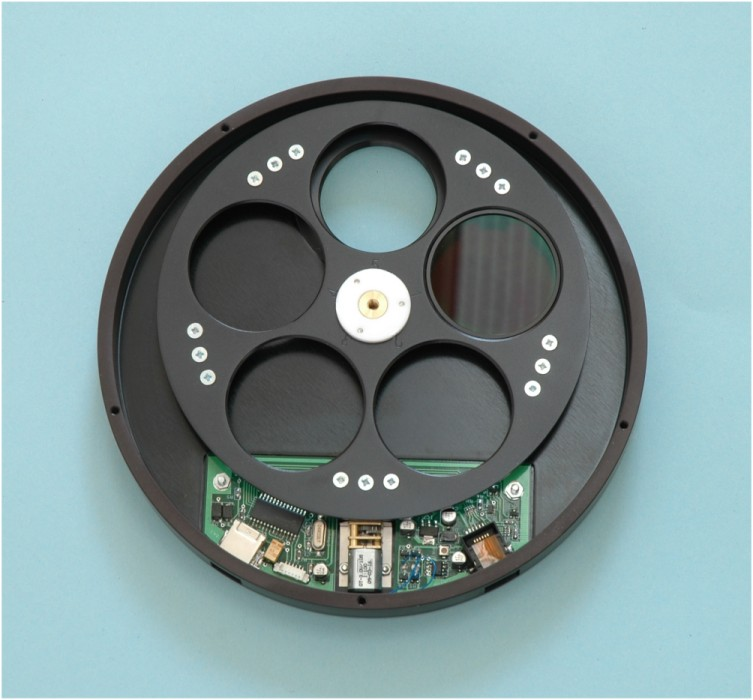
\includegraphics[width=1\textwidth]{../images/portafiltros.jpg}
  \caption{Rueda portafiltros (\url{http://www.lunatico.es/}).}
  \label{fig:diag_scrum}
  \end{center}
\end{figure}

\subsection{Enfocadores}

El \textbf{enfocador} es una pieza fundamental del telescopio. Nos permitirá ver las imágenes formadas tras la reflexión de la luz en el espejo primario y su desviación por el espejo secundario. Para verlas necesitaremos un juego de oculares. La longitud focal de los oculares combinada con la longitud focal de nuestro telescopio nos dará el número de aumentos total del sistema. Dichos oculares están montados en el \textbf{enfocador}, un dispositivo móvil que permitirá mover la posición vertical del ocular para enfocar adecuadamente la imagen.

\bigskip
\begin{figure}[!ht]
  \begin{center}
  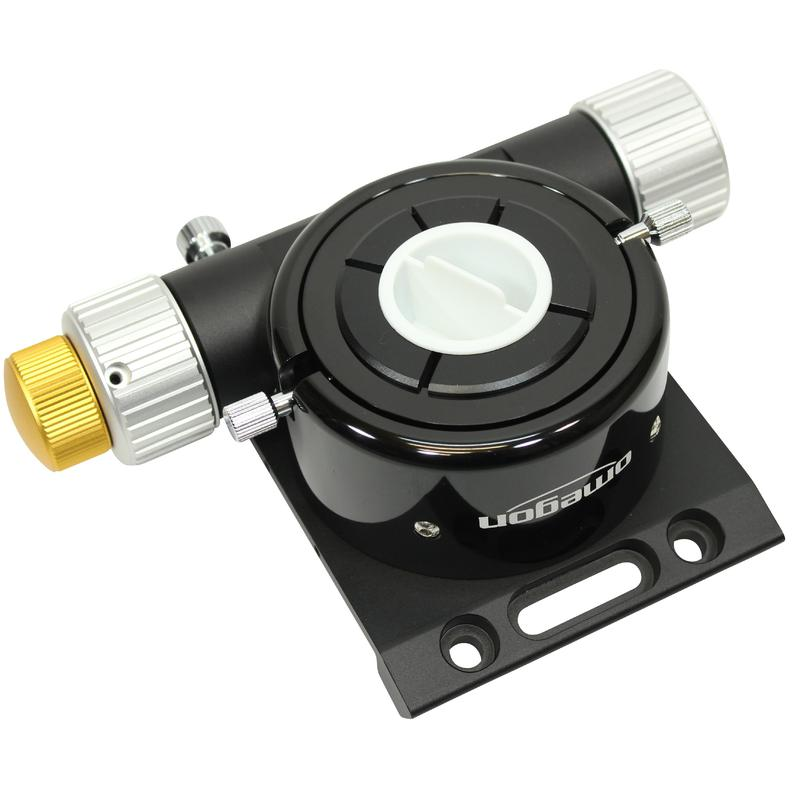
\includegraphics[width=1\textwidth]{../images/enfocador.jpg}
  \caption{Enfocador (\url{http://nimax-img.de/}).}
  \label{fig:diag_scrum}
  \end{center}
\end{figure}
http://cesar-programme.cab.inta-csic.es/

\bigskip
Un ejemplo de enfocador son los de tipo \textbf{Crayford} y los \textbf{rack and pinion}.

\subsection{Cúpulas}
Las \textbf{cúpulas} son recintos cerrados mas o menos grandes que nos permiten albergar y proteger el instrumental astronómico. De esta forma, las \textbf{cúpulas} pueden ser abiertas o cerradas para exponer los instrumentos en el momento de las observaciones.

\bigskip
\begin{figure}[!ht]
  \begin{center}
  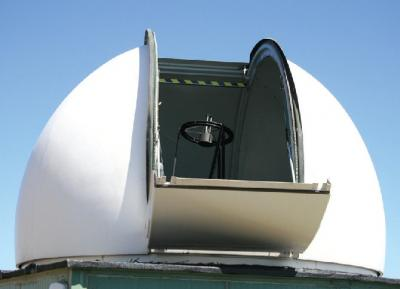
\includegraphics[width=1\textwidth]{../images/cupula.jpg}
  \caption{Cúpula (\url{http://cesar-programme.cab.inta-csic.es/}).}
  \label{fig:diag_scrum}
  \end{center}
\end{figure}
https://www.valkanik.com

\subsection{Ópticas activas/adaptativas}

La \textbf{óptica adaptativa} es una técnica que permite corregir las perturbaciones más importantes que sufren las imágenes astronómicas debido a la atmósfera terrestre. Con este sistema es posible obtener imágenes más nítidas o de mejor resolución espacial. La diferencia que introduce esta técnica es comparable a la que existe entre mirar un objeto situado en el fondo de una piscina con agua o sin agua.

\bigskip
\begin{figure}[!ht]
  \begin{center}
  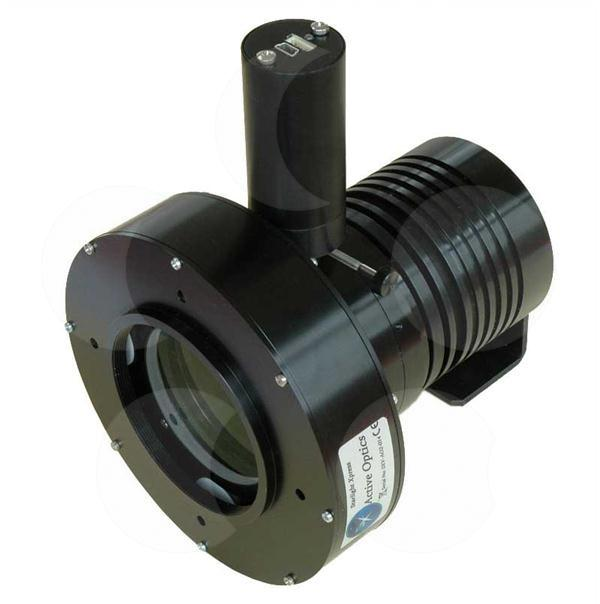
\includegraphics[width=1\textwidth]{../images/optica.jpg}
  \caption{Óptica adaptativa (\url{https://www.valkanik.com}).}
  \label{fig:diag_scrum}
  \end{center}
\end{figure}
http://www.depositohidrografico.com/


\bigskip
Las posibilidades que la óptica adaptativa ofrece a la astronomía son espectaculares. Eliminar las perturbaciones producidas por la atmósfera equivale esencialmente a observar desde el espacio. Las perturbaciones atmosféricas causan una pérdida en nitidez o resolución espacial. Esta pérdida se traduce, por un lado, en una disminuida capacidad para resolver objetos, es decir, para realizar estudios detallados de su morfología. Por otro lado, influye también en la capacidad de detectar objetos débiles, dado que la imagen se dispersa en puntos de luz mayores.

\bigskip
La mejora que introduce la óptica adaptativa se puede cuantificar utilizando la relación entre el tamaño del telescopio y el tamaño de la mejor imagen que puede obtener. El poder de detección de un telescopio aumenta con el diámetro de su espejo primario y disminuye con el tamaño de la imagen que forma de un objeto puntual (de aquí la importancia de la calidad de imagen en un telescopio). Por tanto, la diferencia con un mismo espejo de 10 metros, entre conseguir enfocar imágenes de 0.4 segundos de arco (lo posible en una noche de visibilidad excelente) y una imagen de 0.04 segundos de arco, que debe ser posible con un sistema de óptica adaptativa, equivaldría a tener un espejo primario de 100 metros

\subsection{Estaciones meteorológicas}

Las \textbf{estaciones meteorológicas} son sistemas compuestos por un \textit{``data logger''} y un conjunto de sensores que nos proprcionan datos de las distintas magnitudes meteorológicas, tales como la temperatura, humedad, presión barométrica, etc... permitiéndonos generar modelos a partir de los cuales conocer la situación climática y su posible evolución. 

\bigskip
\begin{figure}[!ht]
  \begin{center}
  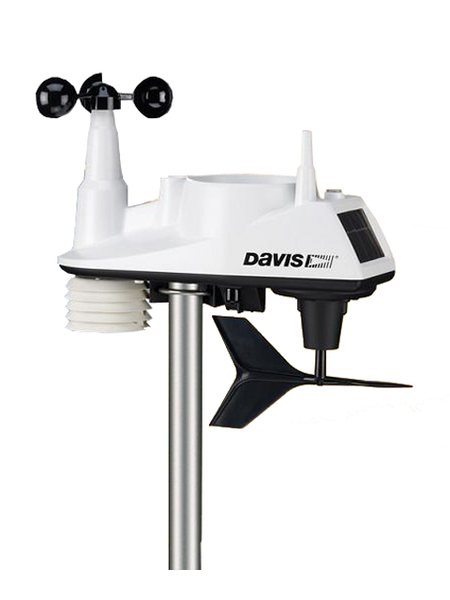
\includegraphics[width=1\textwidth]{../images/estacion.jpg}
  \caption{Estación meteorológica (\url{http://www.depositohidrografico.com/}).}
  \label{fig:diag_scrum}
  \end{center}
\end{figure}


\bigskip
Gracias a los datos aportados por las \textbf{estaciones meteorológicas}, podemos conocer la climatología en el momento de realizar observaciones astronómicas. De esta forma podemos decidir si las condiciones son óptimas, o incluso decidir si debemos cerrar la cúpula para evitar daños en los intrumentos por lluvias o similar. 

\newpage
\section{Control de dispositivos astronómicos}

Actualmente existen diversas formas de controlar los dispositivos astronómicos pero la mayoría presenta los mismos incovenientes:

\begin{itemize}
  \item Normalmente se controlan los dispositivos directamente.
  \item Se conecta el dispositivo a un PC y se trabaja desde él.
  \item Se utilizan herramientas para el control remoto como el \textif{``escritorio remoto''}.
\end{itemize}

\bigskip

Por otro lado, existen estándares como el de \textbf{ASCOM} para instrumental astronómico. Con él, se intenta crear una capa entre los programas para controlar dispositivos astronómicos y los propios dispositivos. \textbf{ASCOM} solo puede utilizarse en sistemas \textit{Microsoft Windows}. Su diseño tiene una relación bastante profunda con el sistema operativo lo cual dificulta el desarrollo basado en red.

\bigskip
\begin{figure}[!ht]
  \begin{center}
    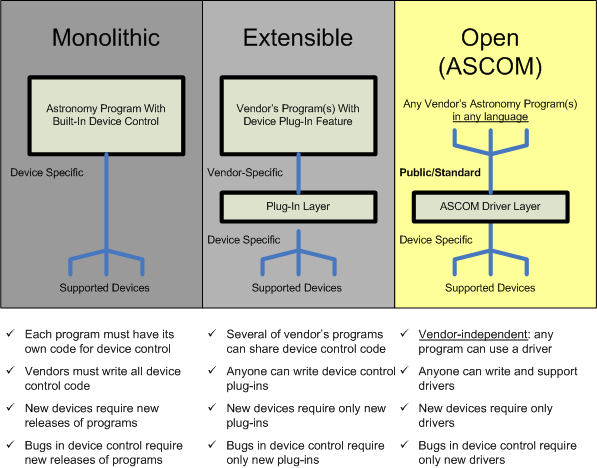
\includegraphics[scale=0.5]{../images/ascom.png}
    \caption{ASCOM Standard (\url{http://ascom-standards.org/})}
    \label{fig:ascom}
  \end{center}
\end{figure}


\newpage
\section{INDI}

\begin{quote}``\textit{The Instrument Neutral Distributed Interface (INDI) Library is a cross-platform software designed for automation & control of astronomical instruments. It supports a wide variety of telescopes, CCDs, focusers , filter wheels..etc, and it has the capability to support virtually any device. INDI is small, flexible, easy to parse, and scalable. It supports common DCS functions such as remote control, data acquisition, monitoring, and a lot more. With INDI, you have a total transparent control over your instruments so you can get more science with less time.}''
\newline(\url{http://indilib.org/about.html})
\end{quote}

\bigskip

El protocolo \textbf{INDI} es una plataforma software diseñada para el control de instrumental astronómico. La biblioteca \textbf{INDI} permite controlar cualquier dispositivo con un driver \textbf{INDI} mediante el paso de archivos XML. Sus principales ventajas frente a otras soluciones para el control de dispositivos son:


\begin{itemize}
  \item Es una biblioteca ligera, flexible y escalable.
  \item Es de código abierto por lo que cualquiera puede ver su código y mejorarlo o crear drivers para cualquier dispositivo
  \item El intercambio de información es mínimo.
  \item Es multiplataforma.
  \item Separa el cliente del servidor.
  \item Los fabricantes comienzan a desarrollar drivers para sus dispositivos o liberan las especificaciones para que la comunidad pueda desarrollarlos.
  \item Existen numerosos clientes INDI como \url{https://edu.kde.org/kstars/}

\end{itemize}

\bigskip
\begin{figure}[!ht]
  \begin{center}
    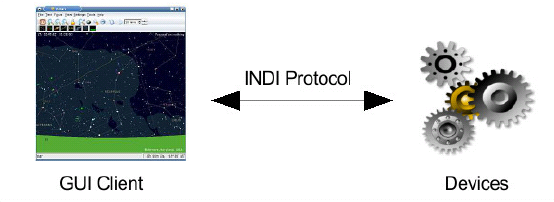
\includegraphics[width=1\textwidth]{../images/Indi_client.png}
    \caption{INDI Client (\url{http://www.indilib.org/})}
    \label{fig:indi_client}
  \end{center}
\end{figure}

\bigskip
\begin{figure}[!ht]
  \begin{center}
    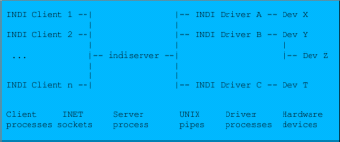
\includegraphics[width=1\textwidth]{../images/Indi_server.png}
    \caption{INDI Server (\url{http://www.indilib.org/})}
    \label{fig:indi_server}
  \end{center}
\end{figure}

\bigskip

\subsection{Breve introducción a INDI}

INDI consiste a su nivel más básico en un protocolo que permite el control, automatización, obtención de datos e intercambio de los mismos entre distintos dispositivos hardware y programas cliente. La idea subyacente en el protocolo INDI es desacoplar aspectos específicos del hardware que se controla de tal manera que cambios en el hardware no impliquen necesariamente cambios en el software (cosa que ocurre en sistemas más habituales donde el el frontend software está fuertemente acoplado con el backend hardware.

\bigskip
Para conseguir un desacople efectivo entre los clientes y el hardware se define un protocolo basado en XML que permite abstraer los dispositivos hardware como conjuntos de propiedades que pueden ser leidas, y modificadas por los clientes (siempre estableciendo las restricciones oportunas).


\subsection{Drivers, Servidores y Clientes INDI}

Pese a que nivel más básico INDI es ``simplemente'' una especificación de un protocolo basado en XML, a un nivel superior se distinguen tres entidades diferentes que interaccionan entre sí para tener un sistema de control plenamente funcional:

\begin{itemize}
  \item \textbf{Drivers:} Son programas que se ejecutarán en la máquina en la que están conectados los dispositivos hardware. Son los encargados de la comunicación directa con los dispositivos y su abstracción a propiedades INDI.
  
  \item \textbf{Servidor:} Es un programa cuya función principal es ejecutar los drivers y permitir la conexión a los mismos por parte de los clientes (funciona de un modo similar a un proxy). Normalmente reside en la máquina donde están conectados los dispositivos, aunque en principio se pueden crear estructuras de red tipo árbol de servidores. El interambio de información entre el servidor y los drivers se realiza utilizando el protocolo INDI.
  
  \item \textbf{Cliente:} Es un programa que permite conectar con uno o más servidores y su función principal e hacer de interfaz con el usuario. Para ello conecta (usualmente a través de la red) con el servidor e intercambia información sobre los dispositivos utilizando el protocolo INDI (FIGURA \ref{fig:indi_server} ). Es interesante recalcar que los clientes pueden ser de cualquier estilo: desde programas con interfaz de usuario avanzadas, hasta programas simples en línea de comandos scripts completamente automáticos que controlen o monitoricen los dispositivos.
\end{itemize}


\subsection{Abstracción de los Dispositivos}

Para conseguir abstraer los dispositivos y que puedan ser controlados o monitorizados por los clientes el protocolo INDI define las llamadas \textit{propiedades}. Las propiedades tienen ciertas características como por ejemplo:

\begin{itemize}
  \item \textbf{Permiso:} Las propiedades tienen uno de 3 posibles permisos:
    \begin{itemize}
     \item \textbf{Lectura y escritura (R/W):} La propiedad puede ser leida y modificada.
     \item \textbf{Solo lectura (RO)}
     \item \textbf{Solo escritura (WO)}
    \end{itemize}

  \item \textbf{Estado:} Las propiedades tienen uno de los siguientes 4 posibles estados:
    \begin{itemize}
     \item \textbf{Ok:} Estado correcto
     \item \textbf{Idle:} Estado indefinido (normalmente la propiedad aun no ha sido usada)
     \item \textbf{Busy:} Está ocupada (probablemente cambiando de valor)
     \item \textbf{Alert:} Ha ocurrido algún problema con la propiedad.
    \end{itemize}
\end{itemize}

\bigskip
Al margen de esas características, hay que mencionar que las propiedades son un conjunto de usualmente uno o más elementos distintos. Es decir, una única propiedad puede agregar varios valores distintos (normalmente relacionados).

Existen 5 tipos de propiedades distintas:

\begin{itemize}
 \item \textbf{Textuales:} Permiten manejar información textual (cadenas de caracteres).
 
 \item \textbf{Numéricas:} Permiten manejar información numérica. Estas propiedades permiten espeificar los rangos de valores válidos así como el formato de visualización del número (entero, flotante, flotante exponencial o sexagesimal).
 
 \item \textbf{Luces:} Permiten manejar ``señales'' o luces que tienen uno de los siguientes cuatro posibles valores:
   \begin{itemize}
     \item \textbf{Ok}
     \item \textbf{Idle}
     \item \textbf{Busy}
     \item \textbf{Alert}
   \end{itemize}


 \item \textbf{Switch:} Permiten manejar valores entre una lista de posibles alternativas. Permiten especificar la regla de selección de cada una de las alternativas:
   \begin{itemize}
     \item \textbf{Una de muchas:} De todas las alternativas, una y solo una debe estar elegida.
     \item \textbf{Como mucho una:} De todas las alternativas se puede elegir una o ninguna.
     \item \textbf{Cualesquiera de muchas:} De todas las alternativas se pueden seleccionar cualquier numero de ella (desde ninguna a todas).

   \end{itemize}
 \item \textbf{BLOB:} Permite manejar valores binarios (como por ejemplo datos de imagen en una cámara).

\end{itemize}



\subsection{Ejemplo de Abstracción de un Dispositivo}

Para comprender mejor el mecanismo de abstracción que aplica INDI, vamos a realizar un ejemplo sencillo de como el programador de un driver abstrae un dispositivo. Supongamos que se trata de una cámara sencilla. La especificación de la cámara dice que su funcionamiento es muy simple: Solo hace falta comunicarle por el puerto serie un comando que incluye el tiempo de exposición de la misma. Una vez mandado ese comando la cámara tomará la fotografía y devolverá los datos de la fotografía en bruto, como un array de valores numéricos (a mayor valor, mayor intensidad luminosa del pixel).

\bigskip
Por tanto, para ofrecer la funcionalidad al cliente INDI, el driver define las siguientes propiedades:

\begin{itemize}
  \item \texttt{Nombre del driver:} Tipo texto, \texttt{RO}. Contendrá el nombre del driver y dispositivo. No cambiará nunca.
  \item \texttt{Tiempo de Exposición:} Tipo numérico, \texttt{R/W}, entre \texttt{0} y \texttt{3600} (segundos). Por defecto \texttt{0}.
  \item \texttt{Imagen:} Tipo BLOB, \texttt{RO}. Contendrá la información binaria de la imagen. En este ejemplo, será una imagen tipo \texttt{PNG}.
\end{itemize}

\bigskip
El driver, además de definir esas propiedades tendrá el siguiente comportamiento general:

\begin{itemize}
 \item Cuando conecte un cliente mandará la información de las tres propiedades.
 \item Quedará a la espera de que cambie el \texttt{tiempo de exposición}.
 \item Cuando el cliente mande un \texttt{tiempo de exposición} nuevo, mandará el comando apropiado a la cámara para que haga la captura de la imagen y esperará a recibir los datos binarios en bruto de la misma.
 \item Una vez recibidos dichos datos binarios los transformará a formato  \texttt{PNG}.
 \item Mandará al cliente nuevos valores para las propiedades de \texttt{tiempo de exposición} (\texttt{0}, para indicar que ya ha acabado la exposición) e \texttt{imagen} (con los datos binarios, el \texttt{PNG}).
\end{itemize}

\subsection{INDI for Java}

La biblioteca \textbf{INDI} está escrita en lenguaje \textbf{C}, pero existe una implementación realizada en Java y que se encuentra en desarrollo. En la página oficial de \textbf{INDI} \url{http://indilib.org/develop/indiforjava.html} podemos encontrar toda la información sobre nuevas versiónes y la documentación para poder utilizarla. La principal ventaja de poder usar Java es que podemos implementar drivers y clientes con la potencia de un lenguaje Orientado a Objetos y combinarlo con otras tecnologías como los dispositivos móviles basados en la plataforma \textbf{Android}


\newpage

\section{Dispositivos Móviles}

Un \textbf{dispositivo móvil} es un tipo de computadora de tamaño pequeño, con capacidad de procesamiento, con conexión a internet, con memoria, diseñados especifcamente para una función pero que pueden llevar a cabo otras funciones más generales.

\bigskip
Los \textbf{dispositivos móviles} hoy en día están integrados en la mayoría de tareas cotidianas de una persona. La tendencía de la sociedad actual nos empuja hacia un mundo cada vez más móvil donde necesitamos estar conectado e interactuar con otros sitemas. Es por ello que la mayoría de soluciones tecnológicas, hayan sido pensadas o no para el sector de los dispositivos móviles, siempre acaba teniendo una versión para éstos.

\bigskip
Paralelamente a la expansión de los \textbf{dispositivos móviles}, se han creado un gran número de sistemas operativos para estos dispositivos entre los que se encuentra:

\begin{itemize}
  \item Android.
  \item iOS.
  \item BlackBerry OS.
  \item Palm OS.
  \item Windows Mobile/Phone.
  \item Symbian.
\end{itemize}

\bigskip
Actualmente \textbf{Android} y \textbf{iOS} copan el 96.3\% del mercado\footnote{Fuente:http://www.idc.com/getdoc.jsp?containerId=prUS25450615.} . Por lo que nos centraremos principalmente en estos sistemas operativos (S.O.) y los \textbf{dispositivos móviles} compatibles con ellos.

\subsection{iOS}

\textbf{iOS} es un S.O. móvil de la compaía \textit{Apple Inc} originalmente desarrollado para el \textit{iPhone}\footnote{Smartphone de la compañia Apple Inc.} y posteriormente introducido en otros \textbf{dispositivos móviles} de la compañía como el iPod touch\footnote{Dispositivo móvil para reproducir multimedia de la compañía Apple Inc} y el iPad\footnote{Tablet de la compañía Apple Inc.}. \textbf{iOS} no puede ser instalado en hardware de terceros.

\bigskip
Actualmente tiene una cuota de mercado aproximadamente del 19.7\%, siendo el segundo S.O. más utilizado.

\bigskip
\textbf{iOS} es un sistema muy estable, diseñado para un hardware muy concreto y por tanto, muy eficiente y depurado. Pero de cara a elegirlo como una opción a la hora de desarrollar una nueva aplicación para \textbf{dispositivos móviles} se debe tener en cuenta los siguientes aspectos:

\begin{itemize}
  \item Hay que pagar una cuota anual de 99\$ para poder publicar aplicaciones en el \textit{Apple Store}\footnote{Tienda de aplicaciónes de la compañia Apple Inc.}. Además si esta licencia, no podremos desarrollar aplicación y cargarla en nuestros dispositivos Apple.
  \item Necesitamos un MAC\footnote{Computadoras personales de la compañia Apple Inc.} ya que las herramientas para el desarrollador solo pueden utilizarse en sus equipos.
  \item Necesitaremos conocer el lenguaje de programación \textbf{Objective-C}
  \item \textbf{iOS} es un sistema de código cerrado que va en contra de la filosofía del \textbf{Software Libre} y el código abierto y reutilizable.

\end{itemize}

\bigskip
Aunque \textbf{iOS} es un sístema muy extendido y con un gran número de usuarios, creemos que no es la mejor opción para orientar una aplicación móvil basada en \textbf{Software Libre} además de la inversión anual requerida para poder publicar una aplicación que prendemos sea gratuita, libre y accesible a cualquier usuario.


\subsection{Android}

\textbf{Android} es un Sistema Operativo basado en un \textbf{núcleo Linux}\footnote{Sistema operativo basado en Unix}. Fue diseñado principalmente para dispositivos móviles con pantalla táctil, relojes inteligentes, televisiones inteligentes y automóviles. Inicialmente pertenecía a la compañía \textbf{Android Inc.} que posteriormente sería adquirida por \textbf{Google}. Actualmente posee la mayor cuota de mercado de aproximadamente el 76.6\%.

\bigskip
Los principales componentes del sistema operativo \textbf{Android} son:


\begin{itemize}
  \item \textbf{Aplicaciones}: Todas las aplicaciones están escritas en lenguaje de programación \textbf{Java}.
  \item \textbf{Framework}\footnote{Marco de trabajo para los desarrolladores}: Los desarrolladores tiene acceso completo a las mismas API's\footnote{Interfaz de programación de aplicaciones (Application Programming Interface)} que utiliza el sistema. La arquitectura está diseñada para simplificar la reutilización de componentes.
  \item \textbf{Runtime de Android}: Adroid incluye un set de bibliotecas base que porporcionanla mayor parte de las funciones disponibles en las bibliotecas base del lenguaje \textbf{Java}. Cada aplicación android corre su propio proceso, con su propia instancia de la máquina virtual \textit{Dalvik}\footnote{Máquina virtual que utiliza la plataforma Android para ejecutar aplicaciones Java.}
  \item \textbf{Núcleo Linux}: Android depende de Linux para los servicios base del sistema como la seguridad, la gestión de memoria, la gestión de procesos, etc. El núcleo Linux también sirve como capa de abstracción entre el hardware y el software.
\end{itemize}

\bigskip
\textbf{Android} no tiene restricciones de uso por lo que puede utilizarse en número muy extenso de dispositivos móviles. Además es un sistema parcialmente de código abierto. Está basado en Linux y la mayoría del código es abierto aunque no todo el sistema lo es.

\bigskip
De cara al desarrollo de aplicaciones móviles, \textbf{Android} es una opción muy recomendable por las siguientes razones:

\begin{itemize}
  \item La arquitectura del sistema (basada en Linux, lenguaje de programación Java,...)
  \item La mayoría de los dispositivos móviles del mundo tienen como sistema operativo a \textbf{Android} por lo que la difusión será mayor que con otros sistemas.
  \item Las herramientas para desarrollar en Android son multiplataforma y gratuitas. Para poder crear y probar una aplicación solo necesitas un ordenador con cualquier sistema operativo, un dispositivo móvil con android y descargar la herramienta para desarrolladores.
  \item Para poder publicar aplicaciones en \textit{Google Play}\footnote{Tienda de aplicaciones para dispositivos Android} hay que pagar 25\$ sin tener renovarlo anualmente y sin ninguna limitación.
\end{itemize}
\chapter{Objetivos}

El objetivo de este proyecto es desarrollar una aplicación para la plataforma \textbf{Android} que implemente un cliente utilizando la  biblioteca \textbf{``INDI for Java''} basado en el \textbf{Software Libre} y que sea fácilmente extensible.

\bigskip
A continuación se describen los objetivos principales a alcanzar:

\begin{itemize}
  \item \textbf{OBJ-1.} Conseguir un cliente funcional capaz de controlar cualquier dispositivo \textbf{INDI}.
  \item \textbf{OBJ-2.} Poder gestionar múltiples conexiones con múltiples dispositivos simultáneamente.
  \item \textbf{OBJ-3.} Fácilmente extensible, permitiendo añadir vistas para propiedades y  dispositivos por parte de desarrolladores ajenos al proyecto.
  \item \textbf{OBJ-4.} Desarrollar la aplicación bajo una licencia de código abierto fomentando la filosofía del \textbf{Software Libre} y la publicación de todo el código.
\end{itemize}

\bigskip
Además de los objetivos principales, se persigue alcanzar los siguientes objetivos:

\begin{itemize}
  \item \textbf{OBJ-S-1.} Desarrollar la aplicación siguiendo los estándares actuales y las recomendaciones para la plataforma \textbf{Android}.
  \item \textbf{OBJ-S-2.} Facilitar la usabilidad mediante un diseño adecuado de las interfaces, adaptándola a los distintos tamaños de pantalla y personalizándolas a las propiedades estándares de \textbf{INDI}.
  \item \textbf{OBJ-S-3.} Desarrollar para incluir un correcto funcionamiento en el mayor número posible de versiones de \textbf{Android}, maximizando el número de dispositivos compatibles.
  \item \textbf{OBJ-S-4.} Añadir una versión estable en \textit{Google Play} y publicar el \textit{APK}\footnote{Paquete para el sistema operativo Android (Application Package File)} para poder descargarlo a través de internet.
  \item \textbf{OBJ-S-5.} Internacionalizar la aplicación (como mínimo en inglés y castellano).
  \item \textbf{OBJ-S-6.} Difusión del software a través de varios canales: google play, página oficial de \textbf{INDI} y desarrollo de una web propia.
\end{itemize}

\bigskip
Para la realización de los objetivos se pondrán en practica los conocimientos alcanzados en;

\begin{itemize}
  \item \textbf{Ingeniería del software} para el análisis del proyecto.
  \item \textbf{Programación orientada a objetos} para la estructura y la organización del código \textbf{Java}.
  \item \textbf{Programación concurrente y sistemas operativos} para la gestión de las distintas hebras y la comunicación entre ellas.
  \item \textbf{Programación de sistemas multimedia} para poder implementar las interfaces de usuario en \textbf{Android} y poder tratar y mostrar imágenes enviadas por los dispositivos.
  \item \textbf{Infraestructura virtual} para poder gestionar los sistemas para realización de test y simulaciones.
  \item \textbf{Transmisión de datos y redes de computadores} para comprender el comportamiento del protocolo \textbf{INDI} y configurar correctamente las redes para las pruebas.
  \item \textbf{Diseño de Aplicaciones para Internet} para añadir código html a las interfaces de \textbf{Android} y para el desarrollo de un portal web que de difusión e información sobre la aplicación.
\end{itemize}

\bigskip
Por otro lado, han sido necesarios alcanzar conocimientos en otras áreas:

\begin{itemize}
  \item \textbf{Astronomía y equipos astronómicos} para entender a los usuarios potenciales y poder acomodar la aplicación a sus necesidades.
  \item \textbf{Android} para conocer las herramientas que ofrece la plataforma y usar las mas adecuadas según las necesidades concretas.
  \item \textbf{Raspberry Pi}\footnote{Ordenador de placa reducida y única de bajo coste.} para montar un servidor permanente de pruebas o acceso público para probar la aplicación
  \item \textbf{Latex}\footnote{Sistema de composición de textos.} para la realización del presente documento y la ampliación de conocimientos para futuros textos científicos.
  \item \textbf{Git} para la gestión de versiones y la publicación de código abierto que permita a otros desarrolladores participar.
\end{itemize}


\section{Alcance de los objetivos}

La aplicación móvil desarrollada debe cumplir los objetivos principales para cubrir una necesidad existente. Actualmente no existe ninguna aplicación móvil basada en \textbf{INDI} para controlar dispositivos astronómicos. Con la realización del proyecto se pretender cubrir dicha necesidad, obteniendo una aplicación estable y que será mantenida y mejorada más allá de la finalización del Proyecto Fin de Grado. Se trata de un proyecto vivo y extensible en el tiempo.

\bigskip
La consecución de alcanzar también los objetivos secundarios tendrá un efecto directo en la difusión de la aplicación y en la satisfacción directa de los usuarios de la misma. Por ello, se comprará una licencia de desarrollador para \textit{Google Play} y se publicará y dará difusión en distintos canales de comunicación como la página oficial \textbf{INDI} y a través de foros y páginas web.


\section{Interdependencia de los objetivos}

El principal objetivo que debe cumplir la aplicación es el \textit{OBJ-1}, aunque todos los objetivos son independientes excepto los objetivos secundarios \textit{OBJ-S-1}, \textit{OBJ-S-2} y \textit{OBJ-S-3}. Seguir los estándares y recomendaciones de la plataforma \textbf{Android} derivará en una mayor compatibilidad con versiones antiguas del sistema operativo y un diseño de la interfaz de usuario más amigable y fácil de usar. 
\chapter{Planificación}

\section{Fases}

El proyecto se divide en una sucesión de fases previamente establecidas que nos ayudará a estructurar, temporizar y evaluar los costes tanto económicos como humanos. Dado que el propio planteamiento del proyecto implica el uso de una serie de tecnologías como \testbf{Android} e \textbf{INDI}, y la necesidad de conocer el campo de la \textbf{astronomía}, se propuso el proyecto con bastante antelación ya que se preveía tener que realizar una fase de familiarización con las tecnologías y campos implicados. Esta fase es bastante extensa ya que se parte de 0.

\begin{itemize}
  \item \textbf{Fase 0:} Planteamiento del problema.
  \item \textbf{Fase 1:} Familiarización con las tecnologías implicadas.
  \item \textbf{Fase 2:} Especificaciones del proyecto.
  \item \textbf{Fase 3:} Análisis y diseño.
  \item \textbf{Fase 4:} Implementación.
  \item \textbf{Fase 5:} Pruebas.
  \item \textbf{Fase 6:} Documentación.
\end{itemize}

\newpage
\section{Estimación de tiempos}

A continuación se muestran las fases con sus actividades principales y la estimación inicial de tiempos.

\begin{itemize}
   \item \textbf{Planteamiento del problema:}
   \begin{itemize}
    \item Priemra reunión con el cliente.
    \item Descripción de los objetivos que se persiguen.
    \item Planteamiento de las posibles tecnologías.
    \item \underline{\textit{Estimación}}: 4 horas.
    \end{itemize}
\end{itemize}

\begin{itemize}
   \item \textbf{Familiarización con las tecnologías implicadas:}
   \begin{itemize}
    \item Android: Generación de aplicaciones.
    \item Android: Generación de interfaces de usuario.
    \item Android: Posibles entornos para el desarrollador
    \item INDI: Comprensión del protocolo.
    \item INDI: Familiarización con la blilbioteca \textit{``INDI for Java''}
    \item Familiarización con el campo de la astronomía.
    \item Realización de pruebas simples para estudiar la viabilidad técnica del proyecto
    \item \underline{\textit{Estimación:}} 80 horas.
   \end{itemize}
\end{itemize}

\begin{itemize}
   \item \textbf{Especificación del proyecto:}
   \begin{itemize}
    \item Tecnoloías elegidas. Entornos de trabajo.
    \item Recursos humanos.
    \item Presupuesto.
    \item Temporización.
    \item \underline{\textit{Estimación:}} 18 horas.
   \end{itemize}
\end{itemize}

\begin{itemize}
   \item \textbf{Análisis y diseño:}
   \begin{itemize}
    \item Análisis de requisitos.
    \item Diagramas.
    \item Metodología de desarrollo.
    \item \underline{\textit{Estimación:}} 36 horas.
   \end{itemize}
\end{itemize}

\begin{itemize}
 \item \textbf{Implementación:}
 \begin{itemize}
  \item Herramientas seleccionadas.
  \item Creación de una aplicación en Android para abrir y cerrar conexiones de red.
  \item Creación de una aplicación en Android para conectarse con un driver INDI.
  \item Creación de una aplicación en Android para poder listar todas las propiedades y dispositivos de una conexión INDI.
  \item Creación de una aplicación en Android para poder interactuar con las porpiedades de los dispositivos de una conexión INDI.
  \item Creación de una aplicación en Android para poder gestionar varias conexiones INDI simultaneamente.
  \item Creación de interfaces de usuario especificas para propiedades concretas y dispositivos concretos.
  \item \underline{\textit{Estimación:}} 180 horas.
 \end{itemize}
\end{itemize}

\begin{itemize}
 \item \textbf{Pruebas:}
 \begin{itemize}
  \item Pruebas de la aplicación en entronos simulados.
  \item Pruebas de la aplicación en entornos reales.
  \item \underline{\textit{Estimación:}} 30 horas.
 \end{itemize}
\end{itemize}

\begin{itemize}
 \item \textbf{Documentación:}
 \begin{itemize}
  \item Documentación de la aplicación.
  \item Manual de usuario.
  \item Documentación del proyecto.
  \item Manual del desarrollador.
  \item \underline{\textit{Estimación:}} 30 horas.
 \end{itemize}
\end{itemize}

\section{Recursos humanos}

Dado que el objetivo es demostrar las capacidades y competencias del alumno a la hora de afrontar un proyecto, el equipo de recursos humanos solo lo formará él, teniendo que afrontar todas las etapas del desarrollo del proyecto.
\newpage
\section{Presupuesto}

Para el presente proyecto se tendrán en cuenta los siguientes costes:

\begin{itemize}
  \item \textbf{Costes por hora de equipo humano:} En este caso son las horas dedicadas al proyecto por parte del alumno. Podemos ver que el total de horas dedicadas son 298 horas. si cuantificamos el precio de desarrollo por hora. Si estimamos el precio por hora en 25\euro tenemos un coste de 7450\euro.
  \item \textbf{Costes asociados a licencias necesarias para publicar o desarrollar el software:} Dado que hemos elegido la plataforma \textbf{Android} y que basamos el proyecto en \textbf{Software Libre} no será necesario realizar ninguna inversión previa. Unicamente debemos tener en cuenta que para poder publicar la aplicación en \textit{Google Play} debemos pagar 25\euro.
  \item \textbf{Costes asociados a los entornos de prueba simulados:} Para poder realizar las pruebas ha sido necesario comprar una \textit{Raspberry Pi B+} que tiene un coste asociado de 35\euro. En ella se alojan los simuladores necesarios para testear las diferentes funciones del software.
  \item \textbf{Costes asociados a los entornos de prueba con equipos:} Los entornos de prueba simulados son limitados, por lo que para poder probar de forma completa el software es necesario adquitir instrumental astronómico. Por ello ha adquirido una montura, un telescopio básico y una cámara basica por 400\euro.
  \item \textbf{Costes asociados a la publicación y difusión a través de internet:} Para dar difusión y permitir descargar la aplicación sin tener que usar \textit{Google Play} se ha desarrollado una página web cuyo coste anual de dominio y hosting asciende a 30\euro al año.
\end{itemize}

\bigskip
Como puede observarse, el coste inicial del proyecto es de \textbf{7940\euro}

\section{SCRUM}

Hasta ahora hemos basado la planificación en una metodología de desarrollo clásica o \textit{en cascada}. Esta metodología se basa en un conocimiento alto de los requisitos del sistema por parte del cliente y una estructura fija y previamente establecida. 

\bigskip
Para el proyecto actual no podemos utilizar este tipo de metodología ya que el cliente no sabe con exactitud lo que quiere, dado que hay una parte de investigación asociada a la consecución del proyecto, lo cual implica la revisión de los requerimientos a lo largo del proceso de desarrollo. Es por ello que se considera más idóneo el uso de una \textbf{metodología ágil} basada en iteraciones incrementales como \textbf{Scrum}.

\bigskip
En \textbf{Scrum} se realizan entregas parciales y regulares del producto final, priorizadas por el beneficio que aportan al receptor del proyecto. Por ello, \textbf{Scrum} está especialmente indicado para proyectos en entornos complejos, donde se necesita obtener resultados pronto, donde los requisitos son cambiantes o poco definidos, donde la innovación, la competitividad, la flexibilidad y la productividad son fundamentales.

\bigskip
En \textbf{Scrum} un proyecto se ejecuta en bloques temporales cortos y fijos (iteraciones de un mes natural y hasta de dos semanas, si así se necesita). Cada iteración tiene que proporcionar un resultado completo, un incremento de producto final que sea susceptible de ser entregado con el mínimo esfuerzo al cliente cuando lo solicite.

\bigskip
Debida a las caracteristicas descritas, se puede aplicar al proyecto dado que en cada iteración el cliente tendrá una aplicación funcional que podrá probar y comprobar si cumple con los objetivos y que nuevos requerimientos son necesarios para, de esta forma, retroalimentar el proceso de desarrollo produciendo una nueva iteración.

\bigskip
En el la figura \ref{fig:diag_scrum} podemos ver el proceso de desarrollo por iteraciones incrementales en \textbf{Scrum}.

\begin{figure}[!ht]
  \begin{center}
  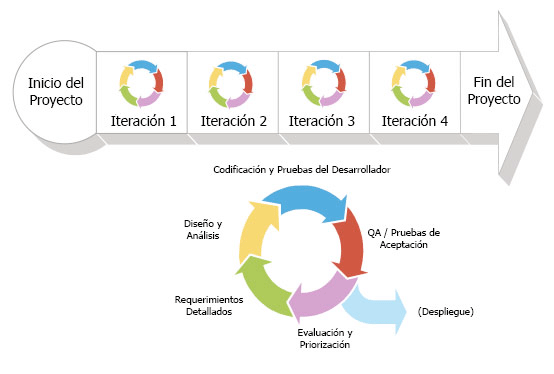
\includegraphics[width=0.8\textwidth]{../images/scrum-iteration-detail-es.png}
  \caption{Proceso de desarrollo Scrum (\url{http://www.qasoluciones.es/metodologia/agile})}
  \label{fig:diag_scrum}
  \end{center}
\end{figure}

Esta metodología redefine las fases en tanto en cuanto ahora debemos repetir n veces las fases de analisis, diseño, implementación, pruebas y documentación. Las horas estimadas son las mimas ya que se repartirían entre las iteraciones. De esta forma el coste del proyecto no se ve incrementado, solo la organización de las tareas y fases de cara al desarrollo del software. 

\section{Temporización}

En la figura \ref{fig:diag_gantt_inicial} se muestra un diagrama de \textbf{Gantt}\footnote{Herramienta gráfica para mostrar la temporización de una serie de tareas} para ilustrar la temporización de las tareas basandonos en la planificación inicial. 

\begin{figure}[!ht]
  \begin{center}
  \includegraphics[width=0.8\textwidth]{../images/diagrama_grantt_inicial.png}
  \caption{Diagrama de Gantt inicial}
  \label{fig:diag_gantt_inicial}
  \end{center}
\end{figure}

\bigskip
Aunque inicialmente se plantea una temporización basada en un número fijo de iteraciones, el proceso de desarrollo hace necesario modificar los planteamientos iniciales de horas, costes y temporización. Por ello, en la figura \ref{fig:diag_gantt_final} puede observarse una diagrama de \textbf{Gantt} con la temporización real.

\begin{figure}[!ht]
  \begin{center}
  \includegraphics[width=0.8\textwidth]{../images/diagrama_grantt_final.png}
  \caption{Diagrama de Gantt final}
  \label{fig:diag_gantt_final}
  \end{center}
\end{figure}

\chapter{Análisis}

En este capítulo vamos a desgranar el proceso de análisis del proyecto, describiendo cada una de las partes que se han realizado.

\section{Análisis de requisitos}

El primer paso en el análisis de un desarrollo software es identificar los requisitos funcionales y no funcionales. Estos requisitos son los que deberá garantizar el producto final y son generados a partir de las entrevistas con el cliente y los objetivos marcados para el software.

\bigskip
Nuestra metodología es ágil basada en iteraciones incrementales por lo que los requisitos son analizados en cada iteración, pudiendo ser modificados según las necesidades.


\subsection{Requisitos funcionales}

Los requisitos funcionales son las características que debe satisfacer el sistema, es decir, todas aquellas funciones que debe cumplir el producto final:

\begin{itemize}
	\item \textbf{RF-1.} Conectarse con un servidor INDI.
	\item \textbf{RF-2.} Gestionar conexiones (crear, editar y borrar).
	\item \textbf{RF-3.} Listar todos los dispositivos de una conexión INDI.
	\item \textbf{RF-4.} Listar todas las propiedades de un dispositivo INDI.
	\item \textbf{RF-5.} Tener más de una conexión INDI simultáneamente.
	\item \textbf{RF-6.} Mostrar un log para cada conexión.
	\item \textbf{RF-7.} Agrupar las propiedades por grupos.
	\item \textbf{RF-8.} Editar las propiedades INDI:
		\begin{itemize}
			\item \textbf{RF-8.1.} Propiedad Blob.
			\item \textbf{RF-8.2.} Propiedad Switch.
			\item \textbf{RF-8.3.} Propiedad Number.
			\item \textbf{RF-8.4.} Propiedad Text.
			\item \textbf{RF-8.5.} Propiedad Light.
		\end{itemize}
\end{itemize}

\subsection{Requisitos no funcionales}

Los requerimientos no funcionales, como su nombre sugiere, son aquellos requerimientos que no se refieren directamente a las funciones específicas que proporciona el sistema, sino a las propiedades emergentes de éste:

\begin{itemize}
  \item \textbf{RN-1.} Las interfaces deben seguir las recomendaciones de diseño establecidas por Android.
  \item \textbf{RN-2.} Se deben usar las clases y elementos de interfaz recomendados para la última versión de Android y usar las bibliotecas de compatibilidad.
  \item \textbf{RN-3.} Controlar la hebra principal para no sobre cargarla, creando nuevas hebras en paralelo mejorando así el rendimiento.
  \item \textbf{RN-4.} Crear interfaces específicas para las propiedades genéricas de INDI y para dispositivos conocidos.
  \item \textbf{RN-5.} Utilizar licencias libres para publicar el proyecto como Software libre
  \item \textbf{RN-6.} Adaptar la aplicación a distintos tamaños de pantalla.
  \item \textbf{RN-7.} Diseñar el software para facilitar la extensibilidad de las vistas de dispositivos y propiedades.
  \item \textbf{RN-8.} Internacionalización de la aplicación: Mínimo inglés y castellano.
\end{itemize}

\section{Casos de uso}

Un caso de uso es una descripción de los pasos o las actividades que deberán realizarse para llevar a cabo algún proceso. Los personajes o entidades que participarán en un caso de uso se denominan actores

\subsection{Descripción de actores}

\begin{itemize}
  \item \textbf{Ac-1.} Usuario.
  \begin{itemize}
   \item Descripción: Persona que utilizará la aplicación.
   \item Características: Es el usuario estándar de la aplicación.
   \item Relaciones: Ninguna.
   \item Atributos: Ninguno.
   \item Comentarios: El usuario no tiene ningún conocimiento previo sobre la aplicación aunque probablemente pueda estar familiarizado con INDI y la astronomía
  \end{itemize}
\end{itemize}

\subsection{Descripción casos de uso}

\begin{itemize}
  \item \textbf{CU-1.} Añadir una conexión.
  \begin{itemize}
    \item \textbf{Actores:} Usuario.
    \item \textbf{Tipo:} Primario, esencial.
    \item \textbf{Referencias:}
    \item \textbf{Precondición:}
    \item \textbf{Postcondición:} La nueva conexión será añadida a la lista y guardada.
    \item \textbf{Autor:} \autor.
    \item \textbf{Versión:} 1.0.
    \item \textbf{Propósito:} Añadir una nueva conexión.
    \item \textbf{Resumen:} El usuario rellenará una serie de campos y marcará unas opciones para añadir una nueva conexión a la lista.
    \end{itemize}
    \begin{table}[!ht]
      \begin{center}
	\begin{tabular}{|l|l|l|l|}
	  \hline
	  \multicolumn{4}{|c|}{{\bf Curso normal}}
	  \\ \hline
	  \multicolumn{2}{|c|}{{\bf Actor}} & \multicolumn{2}{c|}{{\bf Sistema}}
	  \\ \hline
	  {\it 1} & 
	  \begin{tabular}[c]{@{}l@{}}
	    Usuario: Pulsa el botón para\\
	    añadir una nueva conexión.\\
	  \end{tabular} &
	  &
	  \\ \hline
	  &
	  &
	  {\it 2} &
	  \begin{tabular}[c]{@{}l@{}}
	    El sistema muestra el formulario\\
	    para añadir nuevas conexiones. \\
	  \end{tabular}
	  \\ \hline
	  {\it 3} & 
	  \begin{tabular}[c]{@{}l@{}}
	    Usuario: Rellena los campos del \\
	    formulario, marca las opciones  \\
	    y pulsa en el botón de añadir.   \\
	  \end{tabular} &
	  &
	  \\ \hline
	  &
	  &
	  {\it 4} &
	  \begin{tabular}[c]{@{}l@{}}
	    El sistema almacena la conexión\\
	    y la añade a la lista de conexiones.\\
	  \end{tabular}
	  \\ \hline
	\end{tabular}
	\caption{CU-1. Añadir nueva conexión.}
	\label{table:cu_1}
      \end{center}
    \end{table}
    \newpage
    \item \textbf{CU-2.} Editar una conexión.
  \begin{itemize}
    \item \textbf{Actores:} Usuario.
    \item \textbf{Tipo:} Primario, esencial.
    \item \textbf{Referencias:}
    \item \textbf{Precondición:} La conexión debe existir y estar en estado ``desconectada''.
    \item \textbf{Postcondición:} La conexión sera editada y guardada.
    \item \textbf{Autor:} \autor.
    \item \textbf{Versión:} 1.0.
    \item \textbf{Propósito:} Editar una conexión existente.
    \item \textbf{Resumen:} El usuario rellenará una serie de campos y marcará unas opciones para editar la conexión.
    \end{itemize}
    \begin{table}[!ht]
      \begin{center}
	\begin{tabular}{|l|l|l|l|}
	  \hline
	  \multicolumn{4}{|c|}{{\bf Curso normal}}
	  \\ \hline
	  \multicolumn{2}{|c|}{{\bf Actor}} & \multicolumn{2}{c|}{{\bf Sistema}}
	  \\ \hline
	  {\it 1} & 
	  \begin{tabular}[c]{@{}l@{}}
	    Usuario: Pulsa el botón para\\
	    desplegar el menú lateral.\\
	  \end{tabular} &
	  &
	  \\ \hline
	  &
	  &
	  {\it 2} &
	  \begin{tabular}[c]{@{}l@{}}
	    El sistema muestra el menú lateral\\
	    con las conexiones, su estado y sus \\
	    dispositivos.\\
	  \end{tabular}
	  \\ \hline
	  {\it 3} & 
	  \begin{tabular}[c]{@{}l@{}}
	    Usuario: Pulsa el botón editar\\
	    para una conexión concreta.\\
	  \end{tabular} &
	  &
	  \\ \hline
	  &
	  &
	  {\it 4} &
	  \begin{tabular}[c]{@{}l@{}}
	    El sistema muestra el formulario\\
	    para la edición de una conexión. \\
	  \end{tabular}
	  \\ \hline
	  {\it 5} & 
	  \begin{tabular}[c]{@{}l@{}}
	    Usuario: edita los campos del \\
	    formulario, marca las opciones  \\
	    y pulsa en el botón de editar.   \\
	  \end{tabular} &
	  &
	  \\ \hline
	  &
	  &
	  {\it 6} &
	  \begin{tabular}[c]{@{}l@{}}
	    El sistema almacena la conexión\\
	  \end{tabular}
	  \\ \hline
	\end{tabular}
	\caption{CU-2. Editar una conexión.}
	\label{table:cu_2}
      \end{center}
    \end{table}

    \newpage
     \item \textbf{CU-3.} Borrar conexiones.
  \begin{itemize}
    \item \textbf{Actores:} Usuario.
    \item Tipo: Primario, esencial.
    \item \textbf{Referencias:}
    \item \textbf{Precondición:} Las conexiones deben existir.
    \item \textbf{Postcondición:} Las conexiones serán borradas.
    \item \textbf{Autor:} \autor.
    \item \textbf{Versión:} 1.0.
    \item \textbf{Propósito:} Borrar conexiones.
    \item \textbf{Resumen:} El usuario seleccionará de entre las conexiones disponibles, una selección para que sean borradas.
    \end{itemize}
    \begin{table}[!ht]
      \begin{center}
	\begin{tabular}{|l|l|l|l|}
	  \hline
	  \multicolumn{4}{|c|}{{\bf Curso normal}}
	  \\ \hline
	  \multicolumn{2}{|c|}{{\bf Actor}} & \multicolumn{2}{c|}{{\bf Sistema}}
	  \\ \hline
	  {\it 1} & 
	  \begin{tabular}[c]{@{}l@{}}
	    Usuario: Pulsa el botón para\\
	    desplegar el menú superior derecho.\\
	  \end{tabular} &
	  &
	  \\ \hline
	  &
	  &
	  {\it 2} &
	  \begin{tabular}[c]{@{}l@{}}
	    El sistema muestra el menú superior.\\
	  \end{tabular}
	  \\ \hline
	  {\it 3} & 
	  \begin{tabular}[c]{@{}l@{}}
	    Usuario: Pulsa el botón para\\
	    borrar conexiones.\\
	  \end{tabular} &
	  &
	  \\ \hline
	  &
	  &
	  {\it 4} &
	  \begin{tabular}[c]{@{}l@{}}
	    El sistema muestra el formulario\\
	    con una lista de todas las conexiones \\
	  \end{tabular}
	  \\ \hline
	  {\it 5} & 
	  \begin{tabular}[c]{@{}l@{}}
	    Usuario: selecciona aquellas conexiones\\
	    que desee borrar.\\
	  \end{tabular} &
	  &
	  \\ \hline
	  &
	  &
	  {\it 6} &
	  \begin{tabular}[c]{@{}l@{}}
	    El sistema Borra las conexiones\\ 
	    seleccionadas\\
	  \end{tabular}
	  \\ \hline
	\end{tabular}
	\caption{CU-3. Borrar conexiones.}
	\label{table:cu_3}
      \end{center}
    \end{table}

    \newpage
    \item \textbf{CU-4.} Editar los ajustes.
  \begin{itemize}
    \item \textbf{Actores:} Usuario.
    \item \textbf{Tipo:} Opcional, esencial.
    \item \textbf{Referencias:}
    \item \textbf{Precondición:}
    \item \textbf{Postcondición:} Los ajustes serán guardados.
    \item \textbf{Autor:} \autor.
    \item \textbf{Versión:} 1.0.
    \item \textbf{Propósito:} Editar los ajustes.
    \item \textbf{Resumen:} El usuario establecerá las distintas configuraciones.
    \end{itemize}
    \begin{table}[!ht]
      \begin{center}
	\begin{tabular}{|l|l|l|l|}
	  \hline
	  \multicolumn{4}{|c|}{{\bf Curso normal}}
	  \\ \hline
	  \multicolumn{2}{|c|}{{\bf Actor}} & \multicolumn{2}{c|}{{\bf Sistema}}
	  \\ \hline
	  {\it 1} & 
	  \begin{tabular}[c]{@{}l@{}}
	    Usuario: Pulsa el botón para\\
	    desplegar el menú superior derecho.\\
	  \end{tabular} &
	  &
	  \\ \hline
	  &
	  &
	  {\it 2} &
	  \begin{tabular}[c]{@{}l@{}}
	    El sistema muestra el menú superior.\\
	  \end{tabular}
	  \\ \hline
	  {\it 3} & 
	  \begin{tabular}[c]{@{}l@{}}
	    Usuario: Pulsa el botón para\\
	    ver los ajustes.\\
	  \end{tabular} &
	  &
	  \\ \hline
	  &
	  &
	  {\it 4} &
	  \begin{tabular}[c]{@{}l@{}}
	    El sistema muestra la pantalla cin\\
	    con una lista de ajustes y su estado.\\
	  \end{tabular}
	  \\ \hline
	  {\it 5} & 
	  \begin{tabular}[c]{@{}l@{}}
	    Usuario: editada los ajustes que\\ 
	    considere.\\
	  \end{tabular} &
	  &
	  \\ \hline
	  &
	  &
	  {\it 6} &
	  \begin{tabular}[c]{@{}l@{}}
	    El sistema guarda el estado de\\
	    cada configuración.
	  \end{tabular}
	  \\ \hline
	\end{tabular}
	\caption{CU-4. Editar los ajustes.}
	\label{table:cu_4}
      \end{center}
    \end{table}

    \newpage
    \item \textbf{CU-5.} Conectarse a un servidor.
  \begin{itemize}
    \item \textbf{Actores:} Usuario.
    \item \textbf{Tipo:} Primario, esencial.
    \item \textbf{Referencias:}
    \item \textbf{Precondición:} La conexión debe haber sido añadida previamente. La conexión debe estar desconectada.
    \item \textbf{Postcondición:} Se añaden los dispositivos de la conexión a la lista (si los hubiese).
    \item \textbf{Autor:} \autor.
    \item \textbf{Versión:} 1.0.
    \item \textbf{Propósito:} Conectarse a un servidor.
    \item \textbf{Resumen:} El usuario se conectará a un servidor.
    \end{itemize}
    \begin{table}[!ht]
      \begin{center}
	\begin{tabular}{|l|l|l|l|}
	  \hline
	  \multicolumn{4}{|c|}{{\bf Curso normal}}
	  \\ \hline
	  \multicolumn{2}{|c|}{{\bf Actor}} & \multicolumn{2}{c|}{{\bf Sistema}}
	  \\ \hline
	  {\it 1} & 
	  \begin{tabular}[c]{@{}l@{}}
	    Usuario: Pulsa el botón para\\
	    desplegar el menú lateral izquierdo.\\
	  \end{tabular} &
	  &
	  \\ \hline
	  &
	  &
	  {\it 2} &
	  \begin{tabular}[c]{@{}l@{}}
	    El sistema muestra el menú lateral\\
	    izquierdo con la lista de conexiones \\
	    y dispositivos.\\
	  \end{tabular}
	  \\ \hline
	  {\it 3} & 
	  \begin{tabular}[c]{@{}l@{}}
	    Usuario: Pulsa el botón para\\
	    conectarse.\\
	  \end{tabular} &
	  &
	  \\ \hline
	  &
	  &
	  {\it 4a} &
	  \begin{tabular}[c]{@{}l@{}}
	    El sistema esconde el menú lateral y\\
	    realiza la conexión. A partir de ahora \\
	    la conexión se mantiene en segundo plano\\
	    para refrescar los dispositivos añadidos \\
	    o borrados que serán listados al desplegar\\
	    el menú lateral izquierdo.
	  \end{tabular}
	  \\ \hline
	\end{tabular}
	\caption{CU-4. Conectarse a un servidor.}
	\label{table:cu_5}
      \end{center}
    \end{table}
    \begin{table}[!ht]
      \begin{center}
	\begin{tabular}{|l|l|}
	  \hline
	  \multicolumn{2}{|c|}{{\bf Curso alterno}}
	  \\ \hline
	  {\it 4b} &
	  \begin{tabular}[c]{@{}l@{}}
	    Si el servidor no responde, o los datos de la conexión no son\\
	    correctos, el sistema muestra una alerta para informar al \\
	    usuario.\\
	  \end{tabular}\\
	  \hline
	\end{tabular}
	\caption{Curso alterno de CU-5. Conectarse a un servidor.}
	\label{table:ca_cu_5}
      \end{center}
    \end{table}

    \newpage
    \item \textbf{CU-6.} Desconectarse de un servidor.
  \begin{itemize}
    \item \textbf{Actores:} Usuario.
    \item \textbf{Tipo:} Primario, esencial.
    \item \textbf{Referencias:}
    \item \textbf{Precondición:} La conexión debe haber sido añadida previamente. La conexión debe estar conectada.
    \item \textbf{Postcondición:} Se borran de la lista los dispositivos (si los hubiera).
    \item \textbf{Autor:} \autor.
    \item \textbf{Versión:} 1.0.
    \item \textbf{Propósito:} Desconectarse de un servidor.
    \item \textbf{Resumen:} El usuario se desconecta de un servidor.
    \end{itemize}
    \begin{table}[!ht]
      \begin{center}
	\begin{tabular}{|l|l|l|l|}
	  \hline
	  \multicolumn{4}{|c|}{{\bf Curso normal}}
	  \\ \hline
	  \multicolumn{2}{|c|}{{\bf Actor}} & \multicolumn{2}{c|}{{\bf Sistema}}
	  \\ \hline
	  {\it 1} & 
	  \begin{tabular}[c]{@{}l@{}}
	    Usuario: Pulsa el botón para\\
	    desplegar el menú lateral izquierdo.\\
	  \end{tabular} &
	  &
	  \\ \hline
	  &
	  &
	  {\it 2} &
	  \begin{tabular}[c]{@{}l@{}}
	    El sistema muestra el menú lateral\\
	    izquierdo con la lista de conexiones \\
	    y dispositivos.\\
	  \end{tabular}
	  \\ \hline
	  {\it 3} & 
	  \begin{tabular}[c]{@{}l@{}}
	    Usuario: Pulsa el botón para\\
	    desconectarse.\\
	  \end{tabular} &
	  &
	  \\ \hline
	  &
	  &
	  {\it 4} &
	  \begin{tabular}[c]{@{}l@{}}
	    El sistema esconde el menú lateral y\\
	    realiza la desconexión. .
	  \end{tabular}
	  \\ \hline
	\end{tabular}
	\caption{CU-6. Desconectarse de un servidor.}
	\label{table:cu_6}
      \end{center}
    \end{table}

    \newpage
    \item \textbf{CU-7.} Salir de la aplicación.
  \begin{itemize}
    \item \textbf{Actores:} Usuario.
    \item \textbf{Tipo:} Secundario, esencial.
    \item \textbf{Referencias:}
    \item \textbf{Precondición:} La aplicación debe estar iniciada.
    \item \textbf{Postcondición:} Se cierran todas las conexiones, hebras y procesos liberando todos los recursos de la aplicación.
    \item \textbf{Autor:} \autor.
    \item \textbf{Versión:} 1.0.
    \item \textbf{Propósito:} Salir de la aplicación.
    \item \textbf{Resumen:} El usuario cierra la aplicación explícitamente.
    \end{itemize}
    \begin{table}[!ht]
      \begin{center}
	\begin{tabular}{|l|l|l|l|}
	  \hline
	  \multicolumn{4}{|c|}{{\bf Curso normal}}
	  \\ \hline
	  \multicolumn{2}{|c|}{{\bf Actor}} & \multicolumn{2}{c|}{{\bf Sistema}}
	  \\ \hline
	  {\it 1} & 
	  \begin{tabular}[c]{@{}l@{}}
	    Usuario: Pulsa el botón para\\
	    desplegar el menú superior derecho.\\
	  \end{tabular} &
	  &
	  \\ \hline
	  &
	  &
	  {\it 2} &
	  \begin{tabular}[c]{@{}l@{}}
	    El sistema muestra el menú superior.\\
	  \end{tabular}
	  \\ \hline
	  {\it 3} & 
	  \begin{tabular}[c]{@{}l@{}}
	    Usuario: Pulsa el botón salir.\\
	  \end{tabular} &
	  &
	  \\ \hline
	  &
	  &
	  {\it 4} &
	  \begin{tabular}[c]{@{}l@{}}
	    El sistema comprueba cada conexión\\ 
	    y se desconecta de todas, cerrando\\
	    todas las hebras. Después cierra la\\ 
	    aplicación.
	  \end{tabular}
	  \\ \hline
	\end{tabular}
	\caption{CU-7. Salir de la aplicación.}
	\label{table:cu_7}
      \end{center}
    \end{table}

    \newpage
    \item \textbf{CU-8.} Mostrar dispositivo.
  \begin{itemize}
    \item \textbf{Actores:} Usuario.
    \item \textbf{Tipo:} Primario, esencial.
    \item \textbf{Referencias:}
    \item \textbf{Precondición:} La conexión debe haber sido añadida previamente. La conexión debe estar conectada.
    \item \textbf{Postcondición:} Se listan todas las propiedades del dispositivo. Cualquier cambio en las propiedades será mostrado en la lista en tiempo real.
    \item \textbf{Autor:} \autor.
    \item \textbf{Versión:} 1.0.
    \item \textbf{Propósito:} Mostrar las propiedades de un dispositivo.
    \item \textbf{Resumen:} El usuario selecciona un dispositivo para mostrar la lista de sus propiedades.
    \end{itemize}
    \begin{table}[!ht]
      \begin{center}
	\begin{tabular}{|l|l|l|l|}
	  \hline
	  \multicolumn{4}{|c|}{{\bf Curso normal}}
	  \\ \hline
	  \multicolumn{2}{|c|}{{\bf Actor}} & \multicolumn{2}{c|}{{\bf Sistema}}
	  \\ \hline
	  {\it 1} & 
	  \begin{tabular}[c]{@{}l@{}}
	    Usuario: Pulsa el botón para\\
	    desplegar el menú lateral izquierdo.\\
	  \end{tabular} &
	  &
	  \\ \hline
	  &
	  &
	  {\it 2} &
	  \begin{tabular}[c]{@{}l@{}}
	    El sistema muestra el menú lateral\\
	    izquierdo con la lista de conexiones \\
	    y dispositivos.\\
	  \end{tabular}
	  \\ \hline
	  {\it 3} & 
	  \begin{tabular}[c]{@{}l@{}}
	    Usuario: Pulsa sobre el dispositivo\\
	    deseado.\\
	  \end{tabular} &
	  &
	  \\ \hline
	  &
	  &
	  {\it 4} &
	  \begin{tabular}[c]{@{}l@{}}
	    El sistema esconde el menú lateral y\\
	    y muestra una pantalla tabulada con\\
	    todas las vistas especiales que tenga\\
	    el dispositivo (si las tiene) más la\\
	    vista por defecto con la lista de \\
	    de propiedades y la ayuda general de\\
	    la aplicación.
	  \end{tabular}
	  \\ \hline
	\end{tabular}
	\caption{CU-8. Mostrar dispositivo.}
	\label{table:cu_8}
      \end{center}
    \end{table}

    \newpage
    \item \textbf{CU-9.} Cambiar vista de dispositivo.
  \begin{itemize}
    \item \textbf{Actores:} Usuario.
    \item \textbf{Tipo:} Primario, esencial.
    \item \textbf{Referencias:}
    \item \textbf{Precondición:} El usuario debe haber seleccionado un dispositivo (CU-8).
    \item \textbf{Postcondición:}
    \item \textbf{Autor:} \autor.
    \item \textbf{Versión:} 1.0.
    \item \textbf{Propósito:} Cambiar entre las vistas de un dispositivo.
    \item \textbf{Resumen:} El usuario cambia de vista de un dispositivo entre las disponibles.
    \end{itemize}
    \begin{table}[!ht]
      \begin{center}
	\begin{tabular}{|l|l|l|l|}
	  \hline
	  \multicolumn{4}{|c|}{{\bf Curso normal}}
	  \\ \hline
	  \multicolumn{2}{|c|}{{\bf Actor}} & \multicolumn{2}{c|}{{\bf Sistema}}
	  \\ \hline
	  {\it 1} & 
	  \begin{tabular}[c]{@{}l@{}}
	    Usuario: Pulsa sobre el nombre\\
	    de la pestaña correspondiente o \\
	    desliza el dedo por la pantalla.\\
	  \end{tabular} &
	  &
	  \\ \hline
	  &
	  &
	  {\it 2} &
	  \begin{tabular}[c]{@{}l@{}}
	    El sistema muestra la vista correspondiente.\\
	  \end{tabular}
	  \\ \hline
	\end{tabular}
	\caption{CU-9. Cambiar vista de dispositivo.}
	\label{table:cu_9}
      \end{center}
    \end{table}

    \newpage
    \item \textbf{CU-10.} Editar propiedad \textit{text}.
  \begin{itemize}
    \item \textbf{Actores:} Usuario.
    \item \textbf{Tipo:} Primario, esencial.
    \item \textbf{Referencias:}
    \item \textbf{Precondición:} El usuario debe haber seleccionado un dispositivo (CU-8).
    \item \textbf{Postcondición:} La propiedad es editada y enviada al servidor.
    \item \textbf{Autor:} \autor.
    \item \textbf{Versión:} 1.0.
    \item \textbf{Propósito:} Editar una propiedad \textit{text}.
    \item \textbf{Resumen:} El usuario pulsará sobre una propiedad \textit{text} para editarla.
    \end{itemize}
    \begin{table}[!ht]
      \begin{center}
	\begin{tabular}{|l|l|l|l|}
	  \hline
	  \multicolumn{4}{|c|}{{\bf Curso normal}}
	  \\ \hline
	  \multicolumn{2}{|c|}{{\bf Actor}} & \multicolumn{2}{c|}{{\bf Sistema}}
	  \\ \hline
	  {\it 1} & 
	  \begin{tabular}[c]{@{}l@{}}
	    Usuario: Pulsa sobre una propiedad\\
	    de tipo \textit{text}. \\
	  \end{tabular} &
	  &
	  \\ \hline
	  &
	  &
	  {\it 2a} &
	  \begin{tabular}[c]{@{}l@{}}
	    El sistema muestra la vista para la\\
	    edición de las propiedades \textit{text}\\ 
	    con todos los elementos de la\\ 
	    propiedad concreta.\\
	  \end{tabular}
	  \\ \hline
	  {\it 3} & 
	  \begin{tabular}[c]{@{}l@{}}
	    Usuario: edita los elementos que desee\\
	    y pulsa el botón de actualizar\\
	  \end{tabular} &
	  &
	  \\ \hline
	  &
	  &
	  {\it 4} &
	  \begin{tabular}[c]{@{}l@{}}
	    El sistema cierra la vista de edición\\
	    y actualiza la vista de la propiedad.\\
	  \end{tabular}
	  \\ \hline
	\end{tabular}
	\caption{CU-10. Editar una propiedad \textit{text}.}
	\label{table:cu_10}
      \end{center}
    \end{table}

    \begin{table}[!ht]
      \begin{center}
	\begin{tabular}{|l|l|}
	  \hline
	  \multicolumn{2}{|c|}{{\bf Curso alterno}}
	  \\ \hline
	  {\it 2b} &
	  \begin{tabular}[c]{@{}l@{}}
	    Si la propiedad es de solo lectura, el sistema muestra una\\
	    alerta.\\
	  \end{tabular}\\
	  \hline
	\end{tabular}
	\caption{Curso alterno de CU-10. Editar una propiedad \textit{text}.}
	\label{table:ca_cu_10}
      \end{center}
    \end{table}

    \newpage
    \item \textbf{CU-11.} Editar propiedad \textit{number}.
  \begin{itemize}
    \item \textbf{Actores:} Usuario.
    \item \textbf{Tipo:} Primario, esencial.
    \item \textbf{Referencias:}
    \item \textbf{Precondición:} El usuario debe haber seleccionado un dispositivo (CU-8).
    \item \textbf{Postcondición:} La propiedad es editada y enviada al servidor.
    \item \textbf{Autor:} \autor.
    \item \textbf{Versión:} 1.0.
    \item \textbf{Propósito:} Editar una propiedad \textit{number}.
    \item \textbf{Resumen:} El usuario pulsará sobre una propiedad \textit{number} para editarla.
    \end{itemize}
    \begin{table}[!ht]
      \begin{center}
	\begin{tabular}{|l|l|l|l|}
	  \hline
	  \multicolumn{4}{|c|}{{\bf Curso normal}}
	  \\ \hline
	  \multicolumn{2}{|c|}{{\bf Actor}} & \multicolumn{2}{c|}{{\bf Sistema}}
	  \\ \hline
	  {\it 1} & 
	  \begin{tabular}[c]{@{}l@{}}
	    Usuario: Pulsa sobre una propiedad\\
	    de tipo \textit{number}. \\
	  \end{tabular} &
	  &
	  \\ \hline
	  &
	  &
	  {\it 2a} &
	  \begin{tabular}[c]{@{}l@{}}
	    El sistema muestra la vista para la\\
	    edición de las propiedades \textit{number}\\ 
	    con todos los elementos de la\\ 
	    propiedad concreta.\\
	  \end{tabular}
	  \\ \hline
	  {\it 3} & 
	  \begin{tabular}[c]{@{}l@{}}
	    Usuario: edita los elementos que desee\\
	    y pulsa el botón de actualizar\\
	  \end{tabular} &
	  &
	  \\ \hline
	  &
	  &
	  {\it 4a} &
	  \begin{tabular}[c]{@{}l@{}}
	    El sistema cierra la vista de edición\\
	    y actualiza la vista de la propiedad.\\
	  \end{tabular}
	  \\ \hline
	\end{tabular}
	\caption{CU-11 Editar una propiedad \textit{number}.}
	\label{table:cu_11}
      \end{center}
    \end{table}

    \begin{table}[!ht]
      \begin{center}
	\begin{tabular}{|l|l|}
	  \hline
	  \multicolumn{2}{|c|}{{\bf Curso alterno}}
	  \\ \hline
	  {\it 2b} &
	  \begin{tabular}[c]{@{}l@{}}
	    Si la propiedad es de solo lectura, el sistema muestra una\\
	    alerta.\\
	  \end{tabular}\\
	  \hline
	  {\it 4b} &
	  \begin{tabular}[c]{@{}l@{}}
	    Si algún valor de algún elemento editado está fuera de rango\\
	    o tiene un formato erróneo, el sistema mostrará una alerta.\\
	  \end{tabular}
	  \\ \hline
	\end{tabular}
	\caption{Curso alterno de CU-11. Editar una propiedad \textit{number}.}
	\label{table:ca_cu_11}
      \end{center}
    \end{table}

    \newpage
    \item \textbf{CU-12.} Editar propiedad \textit{switch}.
  \begin{itemize}
    \item \textbf{Actores:} Usuario.
    \item \textbf{Tipo:} Primario, esencial.
    \item \textbf{Referencias:}
    \item \textbf{Precondición:} El usuario debe haber seleccionado un dispositivo (CU-8).
    \item \textbf{Postcondición:} La propiedad es editada y enviada al servidor.
    \item \textbf{Autor:} \autor.
    \item \textbf{Versión:} 1.0.
    \item \textbf{Propósito:} Editar una propiedad \textit{switch}.
    \item \textbf{Resumen:} El usuario pulsará sobre una propiedad \textit{switch} para editarla.
    \end{itemize}
    \begin{table}[!ht]
      \begin{center}
	\begin{tabular}{|l|l|l|l|}
	  \hline
	  \multicolumn{4}{|c|}{{\bf Curso normal}}
	  \\ \hline
	  \multicolumn{2}{|c|}{{\bf Actor}} & \multicolumn{2}{c|}{{\bf Sistema}}
	  \\ \hline
	  {\it 1} & 
	  \begin{tabular}[c]{@{}l@{}}
	    Usuario: Pulsa sobre una propiedad\\
	    de tipo \textit{switch}. \\
	  \end{tabular} &
	  &
	  \\ \hline
	  &
	  &
	  {\it 2a} &
	  \begin{tabular}[c]{@{}l@{}}
	    El sistema muestra la vista para la\\
	    edición de las propiedades \textit{switch}\\ 
	    con todos los elementos de la\\ 
	    propiedad concreta.\\
	  \end{tabular}
	  \\ \hline
	  {\it 3} & 
	  \begin{tabular}[c]{@{}l@{}}
	    Usuario: edita los elementos que desee\\
	    y pulsa el botón de actualizar\\
	  \end{tabular} &
	  &
	  \\ \hline
	  &
	  &
	  {\it 4} &
	  \begin{tabular}[c]{@{}l@{}}
	    El sistema cierra la vista de edición\\
	    y actualiza la vista de la propiedad.\\
	  \end{tabular}
	  \\ \hline
	\end{tabular}
	\caption{CU-12 Editar una propiedad \textit{switch}.}
	\label{table:cu_12}
      \end{center}
    \end{table}

    \begin{table}[!ht]
      \begin{center}
	\begin{tabular}{|l|l|}
	  \hline
	  \multicolumn{2}{|c|}{{\bf Curso alterno}}
	  \\ \hline
	  {\it 2b} &
	  \begin{tabular}[c]{@{}l@{}}
	    Si la propiedad es de solo lectura, el sistema muestra una\\
	    alerta.\\
	  \end{tabular}\\
	  \hline
	\end{tabular}
	\caption{Curso alterno de CU-12. Editar una propiedad \textit{switch}.}
	\label{table:ca_cu_12}
      \end{center}
    \end{table}

    \newpage
    \item \textbf{CU-13.} Editar propiedad \textit{blob}.
  \begin{itemize}
    \item \textbf{Actores:} Usuario.
    \item \textbf{Tipo:} Primario, esencial.
    \item \textbf{Referencias:}
    \item \textbf{Precondición:} El usuario debe haber seleccionado un dispositivo (CU-8).
    \item \textbf{Postcondición:} La propiedad es editada y enviada al servidor.
    \item \textbf{Autor:} \autor.
    \item \textbf{Versión:} 1.0.
    \item \textbf{Propósito:} Editar una propiedad \textit{blob}.
    \item \textbf{Resumen:} El usuario pulsará sobre una propiedad \textit{blob} para editarla.
    \end{itemize}
    \begin{table}[!ht]
      \begin{center}
	\begin{tabular}{|l|l|l|l|}
	  \hline
	  \multicolumn{4}{|c|}{{\bf Curso normal}}
	  \\ \hline
	  \multicolumn{2}{|c|}{{\bf Actor}} & \multicolumn{2}{c|}{{\bf Sistema}}
	  \\ \hline
	  {\it 1} & 
	  \begin{tabular}[c]{@{}l@{}}
	    Usuario: Pulsa sobre una propiedad\\
	    de tipo \textit{blob}. \\
	  \end{tabular} &
	  &
	  \\ \hline
	  &
	  &
	  {\it 2a} &
	  \begin{tabular}[c]{@{}l@{}}
	    El sistema muestra la vista para la\\
	    edición de las propiedades \textit{blob}\\ 
	    con todos los elementos de la\\ 
	    propiedad concreta.\\
	  \end{tabular}
	  \\ \hline
	  {\it 3} & 
	  \begin{tabular}[c]{@{}l@{}}
	    Usuario: edita los elementos que desee\\
	    y pulsa el botón de actualizar\\
	  \end{tabular} &
	  &
	  \\ \hline
	  &
	  &
	  {\it 4} &
	  \begin{tabular}[c]{@{}l@{}}
	    El sistema cierra la vista de edición\\
	    y actualiza la vista de la propiedad.\\
	  \end{tabular}
	  \\ \hline
	\end{tabular}
	\caption{CU-13 Editar una propiedad \textit{blob}.}
	\label{table:cu_13}
      \end{center}
    \end{table}

    \begin{table}[!ht]
      \begin{center}
	\begin{tabular}{|l|l|}
	  \hline
	  \multicolumn{2}{|c|}{{\bf Curso alterno}}
	  \\ \hline
	  {\it 2b} &
	  \begin{tabular}[c]{@{}l@{}}
	    Si la propiedad es de solo lectura, el sistema muestra una\\
	    alerta.\\
	  \end{tabular}\\
	  \hline
	\end{tabular}
	\caption{Curso alterno de CU-13. Editar una propiedad \textit{blob}.}
	\label{table:ca_cu_13}
      \end{center}
    \end{table}

    \newpage
    \item \textbf{CU-14.} Editar propiedad \textit{connection}.
  \begin{itemize}
    \item \textbf{Actores:} Usuario.
    \item \textbf{Tipo:} Primario, esencial.
    \item \textbf{Referencias:}
    \item \textbf{Precondición:} El usuario debe haber seleccionado un dispositivo (CU-8).
    \item \textbf{Postcondición:} La propiedad es editada y enviada al servidor.
    \item \textbf{Autor:} \autor.
    \item \textbf{Versión:} 1.0.
    \item \textbf{Propósito:} Editar una propiedad \textit{connection}.
    \item \textbf{Resumen:} El usuario pulsará sobre una propiedad \textit{connection} para editarla.
    \end{itemize}
    \begin{table}[!ht]
      \begin{center}
	\begin{tabular}{|l|l|l|l|}
	  \hline
	  \multicolumn{4}{|c|}{{\bf Curso normal}}
	  \\ \hline
	  \multicolumn{2}{|c|}{{\bf Actor}} & \multicolumn{2}{c|}{{\bf Sistema}}
	  \\ \hline
	  {\it 1} & 
	  \begin{tabular}[c]{@{}l@{}}
	    Usuario: Pulsa sobre una propiedad\\
	    de tipo \textit{connection}. \\
	  \end{tabular} &
	  &
	  \\ \hline
	  &
	  &
	  {\it 2} &
	  \begin{tabular}[c]{@{}l@{}}
	    El sistema muestra la vista para la\\
	    edición de las propiedades \textit{connection}\\ 
	    con un \textit{switch} para conectar\\
	    o desconectar la propiedad.
	  \end{tabular}
	  \\ \hline
	  {\it 3} & 
	  \begin{tabular}[c]{@{}l@{}}
	    Usuario: pulsa sobre el \textit{switch}\\ 
	    para conectar o desconectar la\\ 
	    propiedad y después pulsa en el\\ 
	    botón actualizar.\\
	  \end{tabular} &
	  &
	  \\ \hline
	  &
	  &
	  {\it 4} &
	  \begin{tabular}[c]{@{}l@{}}
	    El sistema cierra la vista de edición\\
	    y actualiza la vista de la propiedad.\\
	  \end{tabular}
	  \\ \hline
	\end{tabular}
	\caption{CU-14 Editar una propiedad \textit{connection}.}
	\label{table:cu_14}
      \end{center}
    \end{table}

    \newpage
    \item \textbf{CU-15.} Editar propiedad \textit{abort}.
  \begin{itemize}
    \item \textbf{Actores:} Usuario.
    \item \textbf{Tipo:} Primario, esencial.
    \item \textbf{Referencias:}
    \item \textbf{Precondición:} El usuario debe haber seleccionado un dispositivo (CU-8).
    \item \textbf{Postcondición:} La propiedad es editada y enviada al servidor.
    \item \textbf{Autor:} \autor.
    \item \textbf{Versión:} 1.0.
    \item \textbf{Propósito:} Editar una propiedad \textit{abort}.
    \item \textbf{Resumen:} El usuario pulsará sobre una propiedad \textit{abort} para editarla.
    \end{itemize}
    \begin{table}[!ht]
      \begin{center}
	\begin{tabular}{|l|l|l|l|}
	  \hline
	  \multicolumn{4}{|c|}{{\bf Curso normal}}
	  \\ \hline
	  \multicolumn{2}{|c|}{{\bf Actor}} & \multicolumn{2}{c|}{{\bf Sistema}}
	  \\ \hline
	  {\it 1} & 
	  \begin{tabular}[c]{@{}l@{}}
	    Usuario: Pulsa sobre una propiedad\\
	    de tipo \textit{abort}. \\
	  \end{tabular} &
	  &
	  \\ \hline
	  &
	  &
	  {\it 2} &
	  \begin{tabular}[c]{@{}l@{}}
	    El sistema muestra la vista para la\\
	    edición de las propiedades \textit{abort}\\ 
	    con un botón para abortar.\\
	  \end{tabular}
	  \\ \hline
	  {\it 3} & 
	  \begin{tabular}[c]{@{}l@{}}
	    Usuario: pulsa sobre el botón\\ 
	    para abortar.\\
	  \end{tabular} &
	  &
	  \\ \hline
	  &
	  &
	  {\it 4} &
	  \begin{tabular}[c]{@{}l@{}}
	    El sistema cierra la vista de edición\\
	    y actualiza la vista de la propiedad.\\
	  \end{tabular}
	  \\ \hline
	\end{tabular}
	\caption{CU-15 Editar una propiedad \textit{abort}.}
	\label{table:cu_15}
      \end{center}
    \end{table}

     \newpage
    \item \textbf{CU-16.} Guardar blob.
  \begin{itemize}
    \item \textbf{Actores:} Usuario.
    \item \textbf{Tipo:} Primario, esencial.
    \item \textbf{Referencias:}
    \item \textbf{Precondición:} El usuario debe haber seleccionado un dispositivo (CU-8). El dispositivo debe tener una propiedad de tipo \textit{blob}.
    \item \textbf{Postcondición:} Se guardará en la carpeta de la aplicación un archivo con el \textit{blob}.
    \item \textbf{Autor:} \autor.
    \item \textbf{Versión:} 1.0.
    \item \textbf{Propósito:} Guardar un \textit{blob}.
    \item \textbf{Resumen:} El usuario guardará un blob que haya recibido.
    \end{itemize}
    \begin{table}[!ht]
      \begin{center}
	\begin{tabular}{|l|l|l|l|}
	  \hline
	  \multicolumn{4}{|c|}{{\bf Curso normal}}
	  \\ \hline
	  \multicolumn{2}{|c|}{{\bf Actor}} & \multicolumn{2}{c|}{{\bf Sistema}}
	  \\ \hline
	  {\it 1} & 
	  \begin{tabular}[c]{@{}l@{}}
	    Usuario: Pulsa sobre el botón guardar\\
	    en la vista de una propiedad\\
	    de tipo \textit{blob}.\\
	  \end{tabular} &
	  &
	  \\ \hline
	  &
	  &
	  {\it 2a} &
	  \begin{tabular}[c]{@{}l@{}}
	    El sistema guarda el blob en la\\
	    carpeta de la aplicación y muestra\\
	    un mensaje por pantalla informando\\
	    del éxito de la acción.\\
	  \end{tabular}
	  \\ \hline
	\end{tabular}
	\caption{CU-16 Guardar un \textit{blob}.}
	\label{table:cu_16}
      \end{center}
    \end{table}

    \begin{table}[!ht]
      \begin{center}
	\begin{tabular}{|l|l|}
	  \hline
	  \multicolumn{2}{|c|}{{\bf Curso alterno}}
	  \\ \hline
	  {\it 2b} &
	  \begin{tabular}[c]{@{}l@{}}
	    Si la propiedad blob no tiene ningún dato que guardar\\
	    se muestra una alerta informando al usuario.\\
	  \end{tabular}\\
	  \hline
	\end{tabular}
	\caption{Curso alterno de CU-16. Guardar un \textit{blob}.}
	\label{table:ca_cu_16}
      \end{center}
    \end{table}

    \newpage
    \item \textbf{CU-17.} Mostrar un blob.
  \begin{itemize}
    \item \textbf{Actores:} Usuario.
    \item \textbf{Tipo:} Primario, esencial.
    \item \textbf{Referencias:}
    \item \textbf{Precondición:} El usuario debe haber seleccionado un dispositivo (CU-8). El dispositivo debe tener una propiedad de tipo \textit{blob}.
    \item \textbf{Postcondición:} Se pasará al sistema operativo \textbf{Android} el archivo para que muestre una lista de posibles aplicaciones instaladas que puedan manejarlo.
    \item \textbf{Autor:} \autor.
    \item \textbf{Versión:} 1.0.
    \item \textbf{Propósito:} Mostrar un \textit{blob}.
    \item \textbf{Resumen:} El usuario guardará un blob que haya recibido.
    \end{itemize}
    \begin{table}[!ht]
      \begin{center}
	\begin{tabular}{|l|l|l|l|}
	  \hline
	  \multicolumn{4}{|c|}{{\bf Curso normal}}
	  \\ \hline
	  \multicolumn{2}{|c|}{{\bf Actor}} & \multicolumn{2}{c|}{{\bf Sistema}}
	  \\ \hline
	  {\it 1} & 
	  \begin{tabular}[c]{@{}l@{}}
	    Usuario: Pulsa sobre el botón mostrar\\
	    en la vista de una propiedad\\
	    de tipo \textit{blob}.\\
	  \end{tabular} &
	  &
	  \\ \hline
	  &
	  &
	  {\it 2a} &
	  \begin{tabular}[c]{@{}l@{}}
	    El sistema guarda el blob en la\\
	    carpeta de la aplicación y envía\\
	    el archivo al sistema operativo\\
	    para poder mostrar el blob con una\\
	    aplicación adecuada según el formato.\\
	  \end{tabular}
	  \\ \hline
	\end{tabular}
	\caption{CU-17 Mostrar un \textit{blob}.}
	\label{table:cu_17}
      \end{center}
    \end{table}

    \begin{table}[!ht]
      \begin{center}
	\begin{tabular}{|l|l|}
	  \hline
	  \multicolumn{2}{|c|}{{\bf Curso alterno}}
	  \\ \hline
	  {\it 2b} &
	  \begin{tabular}[c]{@{}l@{}}
	    Si la propiedad blob no tiene ningún dato que mostrar\\
	    se muestra una alerta informando al usuario.\\
	  \end{tabular}\\
	  \hline
	\end{tabular}
	\caption{Curso alterno de CU-17. Mostrar un \textit{blob}.}
	\label{table:ca_cu_17}
      \end{center}
    \end{table}

    \newpage
     \item \textbf{CU-18.} Ver el log.
  \begin{itemize}
    \item \textbf{Actores:} Usuario.
    \item \textbf{Tipo:} Opcional, esencial.
    \item \textbf{Referencias:}
    \item \textbf{Precondición:}
    \item \textbf{Postcondición:}
    \item \textbf{Autor:} \autor.
    \item \textbf{Versión:} 1.0.
    \item \textbf{Propósito:} Ver el log.
    \item \textbf{Resumen:} El usuario podrá ver el log de cada una de las conexiones guardadas.
    \end{itemize}
    \begin{table}[!ht]
      \begin{center}
	\begin{tabular}{|l|l|l|l|}
	  \hline
	  \multicolumn{4}{|c|}{{\bf Curso normal}}
	  \\ \hline
	  \multicolumn{2}{|c|}{{\bf Actor}} & \multicolumn{2}{c|}{{\bf Sistema}}
	  \\ \hline
	  {\it 1} & 
	  \begin{tabular}[c]{@{}l@{}}
	    Usuario: Pulsa el botón para\\
	    desplegar el menú superior derecho.\\
	  \end{tabular} &
	  &
	  \\ \hline
	  &
	  &
	  {\it 2} &
	  \begin{tabular}[c]{@{}l@{}}
	    El sistema muestra el menú superior.\\
	  \end{tabular}
	  \\ \hline
	  {\it 3} & 
	  \begin{tabular}[c]{@{}l@{}}
	    Usuario: Pulsa el botón para\\
	    ver el log.\\
	  \end{tabular} &
	  &
	  \\ \hline
	  &
	  &
	  {\it 4} &
	  \begin{tabular}[c]{@{}l@{}}
	    El sistema muestra una vista tabulada\\
	    con cada uno de los log que corresponden\\
	    a cada una de las conexiones guardadas
	  \end{tabular}
	  \\ \hline
	\end{tabular}
	\caption{CU-18. Ver el log.}
	\label{table:cu_18}
      \end{center}
    \end{table}

    \newpage
    \item \textbf{CU-19.} Ocultar una propiedad.
  \begin{itemize}
    \item \textbf{Actores:} Usuario.
    \item \textbf{Tipo:} Secundario, esencial.
    \item \textbf{Referencias:}
    \item \textbf{Precondición:} El usuario debe haber seleccionado un dispositivo (CU-8). La propiedad debe estar visible.
    \item \textbf{Postcondición:} La propiedad se maraca como oculta.
    \item \textbf{Autor:} \autor.
    \item \textbf{Versión:} 1.0.
    \item \textbf{Propósito:} Ocultar una propiedad.
    \item \textbf{Resumen:} El usuario ocultará una propiedad visible.
    \end{itemize}
    \begin{table}[!ht]
      \begin{center}
	\begin{tabular}{|l|l|l|l|}
	  \hline
	  \multicolumn{4}{|c|}{{\bf Curso normal}}
	  \\ \hline
	  \multicolumn{2}{|c|}{{\bf Actor}} & \multicolumn{2}{c|}{{\bf Sistema}}
	  \\ \hline
	  {\it 1} & 
	  \begin{tabular}[c]{@{}l@{}}
	    Usuario: Pulsa sobre el icono\\
	    de visibilidad para ocultar una\\
	    propiedad\\
	  \end{tabular} &
	  &
	  \\ \hline
	  &
	  &
	  {\it 2a} &
	  \begin{tabular}[c]{@{}l@{}}
	    El sistema marca la propiedad como \\
	    ``no visible'' y cambia el icono de\\
	    de visibilidad en la vista de la \\
	    propiedad.
	  \end{tabular}
	  \\ \hline
	\end{tabular}
	\caption{CU-19. Ocultar una propiedad.}
	\label{table:cu_19}
      \end{center}
    \end{table}

    \begin{table}[!ht]
      \begin{center}
	\begin{tabular}{|l|l|}
	  \hline
	  \multicolumn{2}{|c|}{{\bf Curso alterno}}
	  \\ \hline
	  {\it 2b} &
	  \begin{tabular}[c]{@{}l@{}}
	    Si la lista de propiedades tiene marcada la opción\\
	    de ``ocultar propiedades'', la propiedad desaparecerá\\
	    de la vista. Si el grupo al que pertenece la propiedad\\
	    no tiene ninguna propiedad visible, también desaparecerá\\
	    de la vista.\\
	  \end{tabular}\\
	  \hline
	\end{tabular}
	\caption{Curso alterno de CU-19. Ocultar una propiedad.}
	\label{table:ca_cu_19}
      \end{center}
    \end{table}

    \newpage
    \item \textbf{CU-20.} Mostrar una propiedad.
  \begin{itemize}
    \item \textbf{Actores:} Usuario.
    \item \textbf{Tipo:} Secundario, esencial.
    \item \textbf{Referencias:}
    \item \textbf{Precondición:} El usuario debe haber seleccionado un dispositivo (CU-8). La propiedad debe estar ``no visible''. Debe estar activada la opción de ``ver todas las propiedades'' para que las que estén marcadas como ocultas se añadan también a la vista
    \item \textbf{Postcondición:} La propiedad se maraca como visible.
    \item \textbf{Autor:} \autor.
    \item \textbf{Versión:} 1.0.
    \item \textbf{Propósito:} Mostrar una propiedad.
    \item \textbf{Resumen:} El usuario marcará una propiedad como visible.
    \end{itemize}
    \begin{table}[!ht]
      \begin{center}
	\begin{tabular}{|l|l|l|l|}
	  \hline
	  \multicolumn{4}{|c|}{{\bf Curso normal}}
	  \\ \hline
	  \multicolumn{2}{|c|}{{\bf Actor}} & \multicolumn{2}{c|}{{\bf Sistema}}
	  \\ \hline
	  {\it 1} & 
	  \begin{tabular}[c]{@{}l@{}}
	    Usuario: Pulsa sobre el icono\\
	    de visibilidad para marcar una\\
	    propiedad como visible.\\
	  \end{tabular} &
	  &
	  \\ \hline
	  &
	  &
	  {\it 2} &
	  \begin{tabular}[c]{@{}l@{}}
	    El sistema marca la propiedad como \\
	    visible y cambia el icono de\\
	    de visibilidad en la vista de la \\
	    propiedad.
	  \end{tabular}
	  \\ \hline
	\end{tabular}
	\caption{CU-20. Mostrar una propiedad.}
	\label{table:cu_20}
      \end{center}
    \end{table}

    \newpage
    \item \textbf{CU-21.} Activar la visibilidad de todas las propiedades ocultas.
  \begin{itemize}
    \item \textbf{Actores:} Usuario.
    \item \textbf{Tipo:} Secundario, esencial.
    \item \textbf{Referencias:}
    \item \textbf{Precondición:} El usuario debe haber seleccionado un dispositivo (CU-8).
    \item \textbf{Postcondición:} Se muestran todas las propiedades sea cual sea su visibilidad.
    \item \textbf{Autor:} \autor.
    \item \textbf{Versión:} 1.0.
    \item \textbf{Propósito:} Activar la visibilidad de todas las propiedades ocultas.
    \item \textbf{Resumen:} El usuario activa la visibilidad de todas las propiedades, estén marcadas como ocultas o no.
    \end{itemize}
    \begin{table}[!ht]
      \begin{center}
	\begin{tabular}{|l|l|l|l|}
	  \hline
	  \multicolumn{4}{|c|}{{\bf Curso normal}}
	  \\ \hline
	  \multicolumn{2}{|c|}{{\bf Actor}} & \multicolumn{2}{c|}{{\bf Sistema}}
	  \\ \hline
	  {\it 1} & 
	  \begin{tabular}[c]{@{}l@{}}
	    Usuario: Pulsa sobre el botón\\
	    flotante para activar la visibilidad\\
	    de todas las propiedades.\\
	  \end{tabular} &
	  &
	  \\ \hline
	  &
	  &
	  {\it 2} &
	  \begin{tabular}[c]{@{}l@{}}
	    El sistema refresca la lista de\\
	    propiedades añadiéndolas todas\\
	    aunque su estado sea ``no visible''.\\
	  \end{tabular}
	  \\ \hline
	\end{tabular}
	\caption{CU-21. Activar la visibilidad de todas las propiedades ocultas.}
	\label{table:cu_21}
      \end{center}
    \end{table}

    \newpage
    \item \textbf{CU-22.} Desactivar la visibilidad de todas las propiedades ocultas.
  \begin{itemize}
    \item \textbf{Actores:} Usuario.
    \item \textbf{Tipo:} Secundario, esencial.
    \item \textbf{Referencias:}
    \item \textbf{Precondición:} El usuario debe haber seleccionado un dispositivo (CU-8).
    \item \textbf{Postcondición:} Se ocultan todas las propiedades cuyo estado esa ``no visible''.
    \item \textbf{Autor:} \autor.
    \item \textbf{Versión:} 1.0.
    \item \textbf{Propósito:} Desactivar la visibilidad de todas las propiedades ocultas.
    \item \textbf{Resumen:} El usuario desactiva la visibilidad de todas las propiedades con el estado ``no visible''.
    \end{itemize}
    \begin{table}[!ht]
      \begin{center}
	\begin{tabular}{|l|l|l|l|}
	  \hline
	  \multicolumn{4}{|c|}{{\bf Curso normal}}
	  \\ \hline
	  \multicolumn{2}{|c|}{{\bf Actor}} & \multicolumn{2}{c|}{{\bf Sistema}}
	  \\ \hline
	  {\it 1} & 
	  \begin{tabular}[c]{@{}l@{}}
	    Usuario: Pulsa sobre el botón\\
	    flotante para desactivar la \\
	    visibilidad de todas las propiedades\\
	    ocultas.\\
	  \end{tabular} &
	  &
	  \\ \hline
	  &
	  &
	  {\it 2} &
	  \begin{tabular}[c]{@{}l@{}}
	    El sistema refresca la lista de\\
	    propiedades mostrando solo\\
	    aquellas que estén visibles.\\
	  \end{tabular}
	  \\ \hline
	\end{tabular}
	\caption{CU-21. Desactivar la visibilidad de todas las propiedades ocultas.}
	\label{table:cu_22}
      \end{center}
    \end{table}

    \newpage
    \item \textbf{CU-23.} Expandir un grupo.
  \begin{itemize}
    \item \textbf{Actores:} Usuario.
    \item \textbf{Tipo:} Secundario, esencial.
    \item \textbf{Referencias:}
    \item \textbf{Precondición:} El usuario debe haber seleccionado un dispositivo (CU-8). El grupo debe estar contraído.
    \item \textbf{Postcondición:} se expande el grupo seleccionado.
    \item \textbf{Autor:} \autor.
    \item \textbf{Versión:} 1.0.
    \item \textbf{Propósito:} Expandir un grupo.
    \item \textbf{Resumen:} El usuario Expande uno de los grupos de la lista que esté contraído.
    \end{itemize}
    \begin{table}[!ht]
      \begin{center}
	\begin{tabular}{|l|l|l|l|}
	  \hline
	  \multicolumn{4}{|c|}{{\bf Curso normal}}
	  \\ \hline
	  \multicolumn{2}{|c|}{{\bf Actor}} & \multicolumn{2}{c|}{{\bf Sistema}}
	  \\ \hline
	  {\it 1} & 
	  \begin{tabular}[c]{@{}l@{}}
	    Usuario: Pulsa sobre el nombre\\
	    del grupo que desee expandir.\\
	  \end{tabular} &
	  &
	  \\ \hline
	  &
	  &
	  {\it 2} &
	  \begin{tabular}[c]{@{}l@{}}
	    El sistema refresca la lista de\\
	    propiedades mostrando el grupo\\
	    expandido y todas las propiedades\\
	    que contenga.\\
	  \end{tabular}
	  \\ \hline
	\end{tabular}
	\caption{CU-23. Expandir un grupo.}
	\label{table:cu_23}
      \end{center}
    \end{table}

    \newpage
    \item \textbf{CU-24.} Contraer un grupo.
  \begin{itemize}
    \item \textbf{Actores:} Usuario.
    \item \textbf{Tipo:} Secundario, esencial.
    \item \textbf{Referencias:}
    \item \textbf{Precondición:} El usuario debe haber seleccionado un dispositivo (CU-8). El grupo debe estar expandido.
    \item \textbf{Postcondición:} se contrae el grupo seleccionado.
    \item \textbf{Autor:} \autor.
    \item \textbf{Versión:} 1.0.
    \item \textbf{Propósito:} Contraer un grupo.
    \item \textbf{Resumen:} El usuario contrae uno de los grupos de la lista que esté expandido.
    \end{itemize}
    \begin{table}[!ht]
      \begin{center}
	\begin{tabular}{|l|l|l|l|}
	  \hline
	  \multicolumn{4}{|c|}{{\bf Curso normal}}
	  \\ \hline
	  \multicolumn{2}{|c|}{{\bf Actor}} & \multicolumn{2}{c|}{{\bf Sistema}}
	  \\ \hline
	  {\it 1} & 
	  \begin{tabular}[c]{@{}l@{}}
	    Usuario: Pulsa sobre el nombre\\
	    del grupo que desee contraer.\\
	  \end{tabular} &
	  &
	  \\ \hline
	  &
	  &
	  {\it 2} &
	  \begin{tabular}[c]{@{}l@{}}
	    El sistema refresca la lista de\\
	    propiedades mostrando el grupo\\
	    contraído.\\
	  \end{tabular}
	  \\ \hline
	\end{tabular}
	\caption{CU-24. Contraer un grupo.}
	\label{table:cu_24}
      \end{center}
    \end{table}
    
    \newpage
    \item \textbf{CU-25.} Abrir la aplicación.
  \begin{itemize}
    \item \textbf{Actores:} Usuario.
    \item \textbf{Tipo:} primaria, esencial.
    \item \textbf{Referencias:}
    \item \textbf{Precondición:}
    \item \textbf{Postcondición:} La aplicación queda iniciada. Si alguna conexión tiene activada la opción de ``autoconectar'', se realizará la conexión con el servidor.
    \item \textbf{Autor:} \autor.
    \item \textbf{Versión:} 1.0.
    \item \textbf{Propósito:} Iniciar la aplicación.
    \item \textbf{Resumen:} El usuario inicia la aplicación.
    \end{itemize}
    \begin{table}[!ht]
      \begin{center}
	\begin{tabular}{|l|l|l|l|}
	  \hline
	  \multicolumn{4}{|c|}{{\bf Curso normal}}
	  \\ \hline
	  \multicolumn{2}{|c|}{{\bf Actor}} & \multicolumn{2}{c|}{{\bf Sistema}}
	  \\ \hline
	  {\it 1} & 
	  \begin{tabular}[c]{@{}l@{}}
	    Usuario: Pulsa sobre el icono\\
	    de la aplicación.\\
	  \end{tabular} &
	  &
	  \\ \hline
	  &
	  &
	  {\it 2} &
	  \begin{tabular}[c]{@{}l@{}}
	    El sistema carga las configuraciones\\
	    o las crea en caso de no existir. Después\\
	    muestra la interfaz de la aplicación\\
	    mostrando la sección de ayuda.\\
	  \end{tabular}
	  \\ \hline
	\end{tabular}
	\caption{CU-25. Iniciar la aplicación.}
	\label{table:cu_25}
      \end{center}
    \end{table}

\end{itemize}

\newpage
\section{Diagramas de casos de uso}

Los diagramas de casos de uso sirven para representar los relaciones que existen entre los diferentes actores y el sistema. Dado que en nuestro caso solo hay un actor, todos los casos de uso son iniciados por él.

\bigskip

\begin{figure}[!ht]
  \begin{center}
  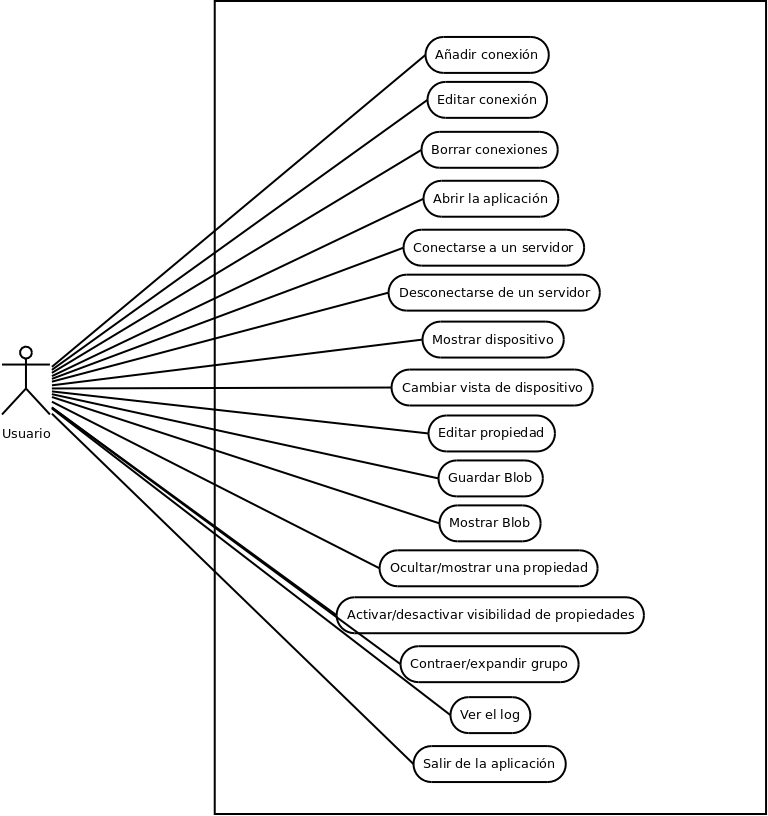
\includegraphics[width=1\textwidth]{../images/diagrama_casos_de_uso.png}
  \caption{Diagrama de casos de uso.}
  \label{fig:diag_scrum}
  \end{center}
\end{figure}

\newpage
\section{Storyboard}

A continuación, en la figura \ref{fig:storyboard} se muestra el storyboard de la aplicación, donde se pueden ver las distintas pantallas por las que puede pasar la aplicación.

\begin{figure}[!ht]
  \begin{center}
  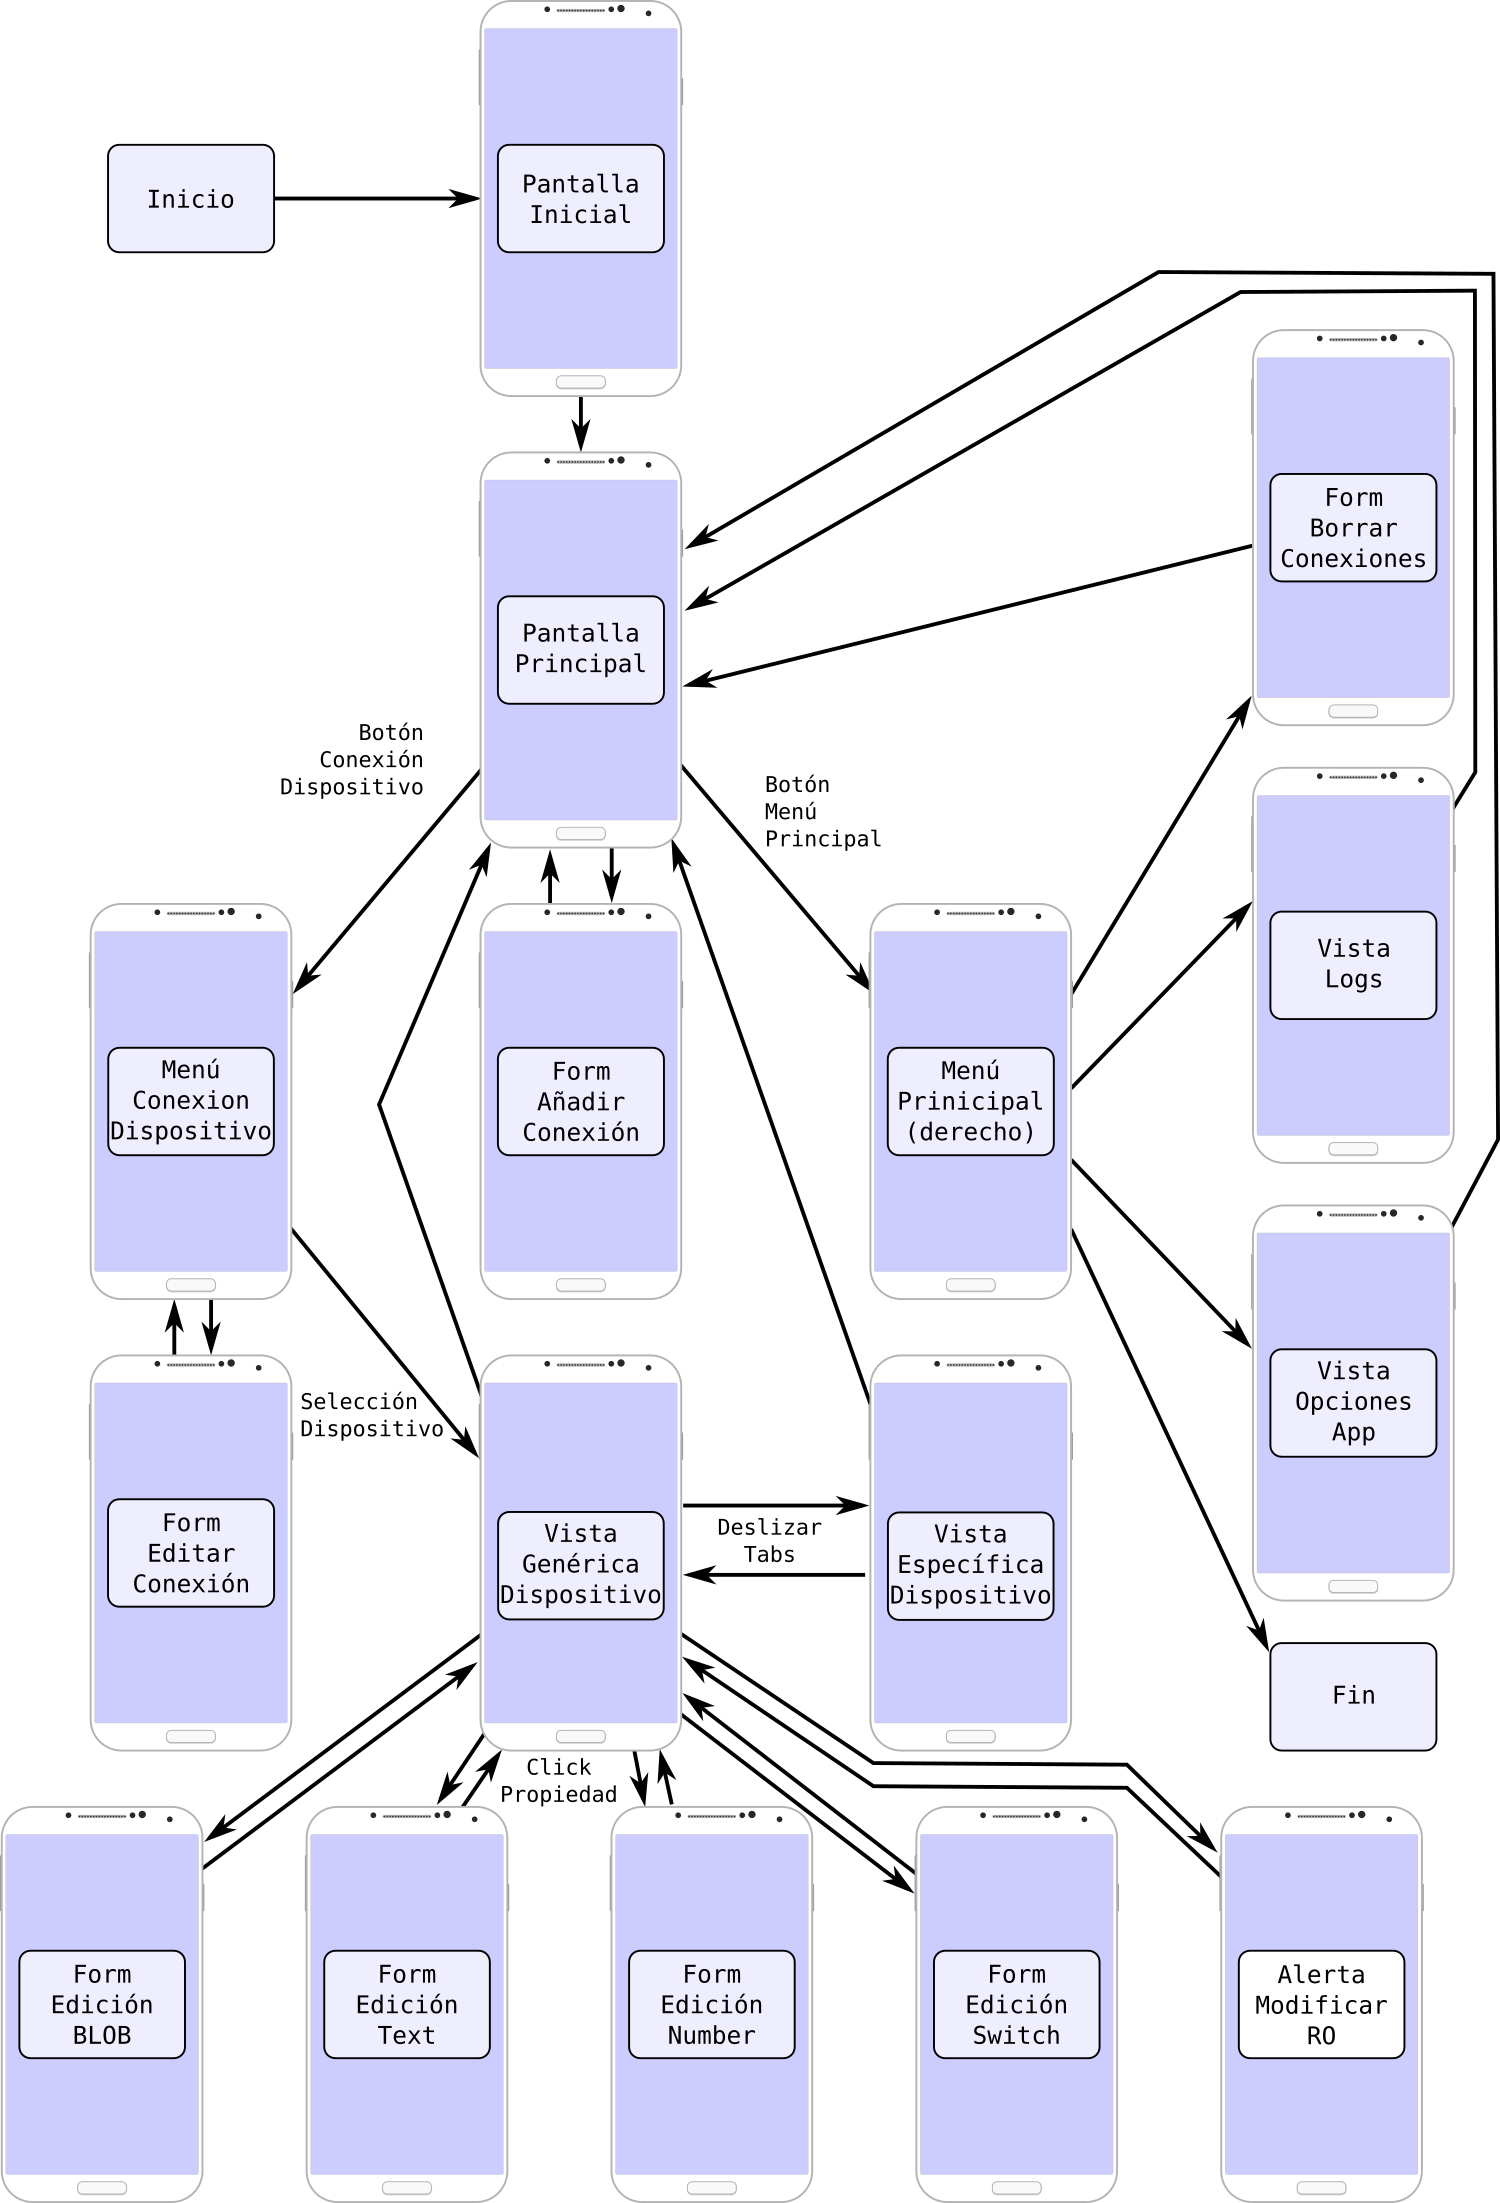
\includegraphics[width=1\textwidth]{../images/storyboard.png}
  \caption{Storyboard de la aplicación.}
  \label{fig:storyboard}
  \end{center}
\end{figure}
\chapter{Diseño e Implementación}

El proyecto tiene dos partes claramente diferenciadas a la hora de plantear el diseño:

\begin{itemize}
  \item \textbf{Diseño de clases.}
  \item \textbf{Diseño de las interfaces de usuario.}
  \item \textbf{Mecanismo de adición de vistas.}
\end{itemize}

Además, hay que tener en cuenta que uno de los objetivos principales es que la aplicación sea fácilmente extensible y que permita añadir nuevas interfaces de usuario para propiedades y dispositivos por lo que es parte importante de la fase de diseño, en la que se describirán todos detalladamente.

\bigskip
\section{Diseño de clases}

En todo proyecto de software es muy importante diseñar correctamente las clases antes de comenzar la fase de implementación. Un mal diseño puede provocar retrasos en la fase de implementación, incluso obligando a retroceder y rediseñarlas.

\bigskip
Podemos dividir el diseño en cuatro bloques:

\begin{itemize}
  \item \textbf{Diseño de las actividades de Android.}
  \item \textbf{Diseño del cliente INDI.}
  \item \textbf{Diseño de las clases manejadoras de propiedades.}
  \item \textbf{Diseño de las clases manejadoras de dispositivos.}
\end{itemize}

\newpage
\subsection{Diseño de las actividades de Android}

Las actividades en android son el cuerpo principal de las aplicaciones. Son ejecutadas en la hebra principal del sistema y gestionan la interfaz principal. Se pueden tener tantas actividades como se desee. En nuestro caso tenemos dos actividades:


\begin{itemize}
  \item \textbf{Front activity}
  \item \textbf{Main activity}
\end{itemize}

\subsubsection{Front activity}

Esta actividad inicia la aplicación, mostrando una pantalla de inicio con la información como portada. Una vez lanzada la aplicación esta actividad no volverá a ejecutarse a no ser que el sistema cierre la aplicación o que lo haga el usuario explícitamente. Como podemos ver en el diagrama de la figura \ref{fig:diag_front}, la actividad solo tiene una clase que hereda de \textit{AppCompatActivity}. Esta clase pertenece a la biblioteca de compatibilidad de \textbf{android}. Además, esta actividad tiene un objeto de la clase \textit{UpdateProgress}. Esta clase sirve para ejecutar código en una hebra separada en la que controlar el progreso.

\bigskip
\begin{figure}[!ht]
  \begin{center}
  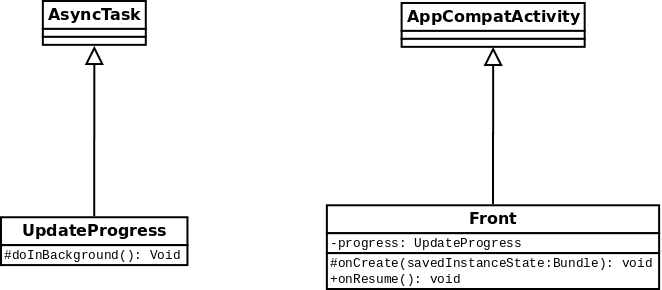
\includegraphics[width=1\textwidth]{../images/front_diag.png}
  \caption{Diagrama de clases de la actividad front}
  \label{fig:diag_front}
  \end{center}
\end{figure}


\subsubsection{Main activity}

La actividad principal es el núcleo de la aplicación. Esta clase es la más importante ya que su ciclo de vida condiciona el ciclo de vida de la aplicación. Es por ello que esta clase es la más compleja. En la figura \ref{fig:diag_main_activity} podemos ver el diagrama de clases. Las clases que no contienen ninguna especificación pertenecen a \textbf{Android} y simplemente se añaden para indicar las relaciones que las clases implementadas.

\bigskip
Dado que esta clase es la responsable de la visualización de los distintos menús, necesitamos declarar objetos de las clases que representan cada uno de los elementos visuales principales, tales como \textit{NavigationView}\cite{HTMMDND} o \textit{TabLayout}\cite{ATLWSV}.

\bigskip
Por otro lado, la actividad implementa una serie de escuchadores que le permiten capturar los eventos disparados por los distintos botones de la interfaz de usuario para realizar las acciones oportunas.

\bigskip
Además de estas clases, se ha diseñado la clase \textit{Settings} que representa las configuraciones generales de la aplicación: notificaciones y carpeta por defecto.

\bigskip
En el diagrama también podemos ver la clase \textit{Connection}. Esta clase representa las conexiones con el servidor y es por ella que se describen en el apartado correspondiente.


\bigskip
\begin{figure}[!ht]
  \begin{center}
  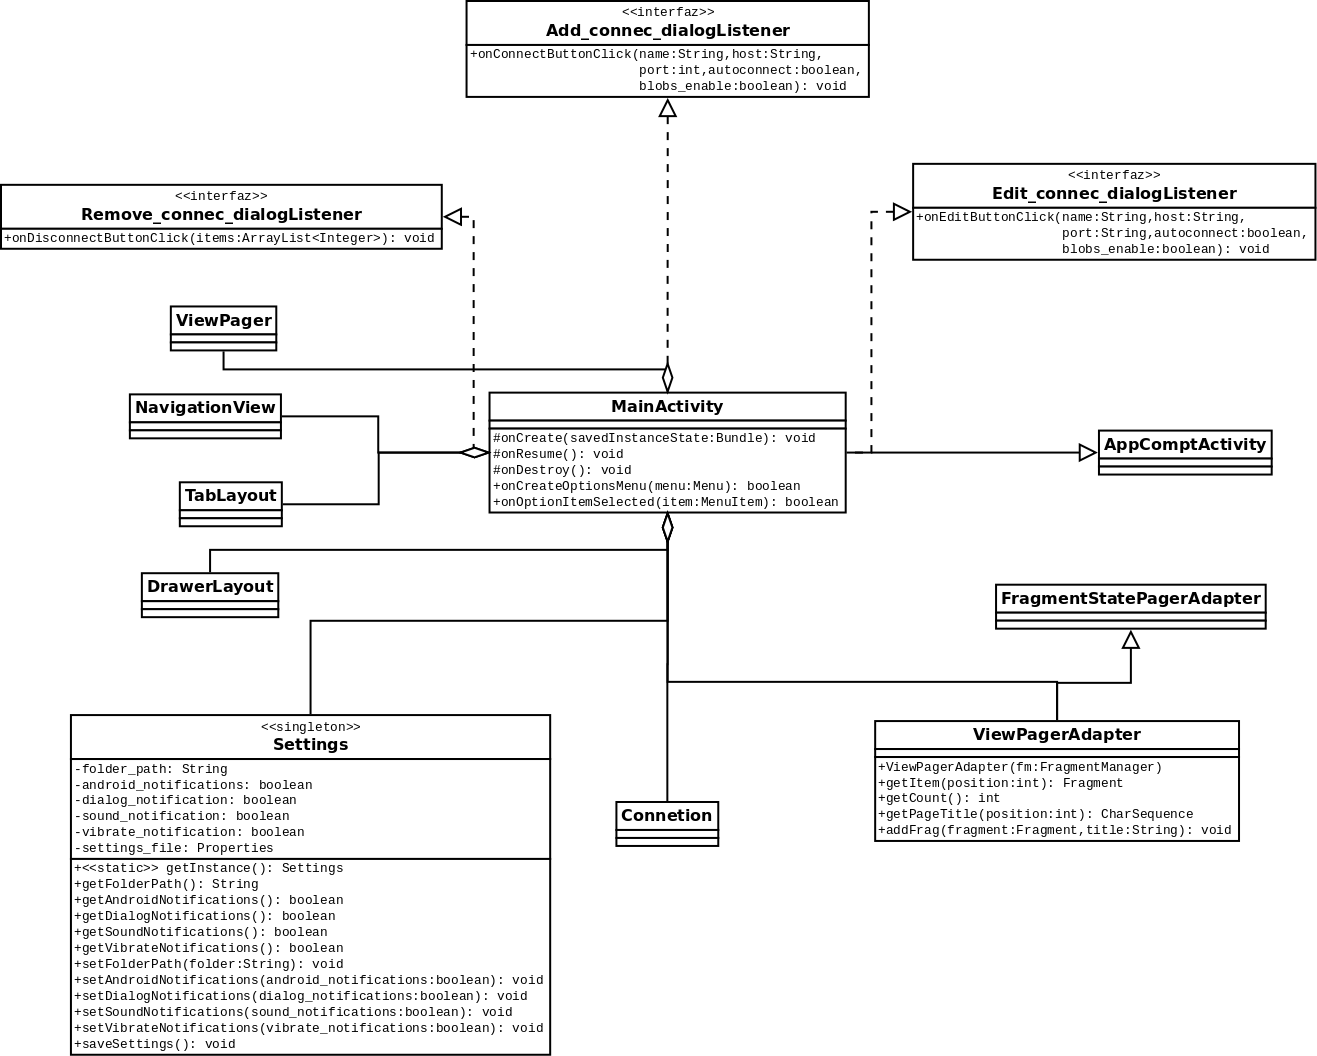
\includegraphics[width=1\textwidth]{../images/main_activity.png}
  \caption{Diagrama de clases de la actividad principal}
  \label{fig:diag_main_activity}
  \end{center}
\end{figure}


\newpage
\subsection{Diseño del cliente INDI}

La aplicación se basa en integrar la biblioteca \textbf{``INDI for Java''} para poder crear un cliente que nos permita conectarnos a cualquier servidor. Las conexiones se hacen creando conexiones TCP/IP a través de la red. \textbf{Android} establece unas restricciones muy fuertes respecto a la apertura y cierre de \textit{sockets} de red. Dado que la arquitectura del sistema esta basada en una única hebra principal que gestiona la interfaz de usuario, si iniciamos algún proceso que pueda bloquear dicha hebra, bloquearíamos todo el sistema. Por ello cualquier proceso de comunicación debe ejecutarse en una hebra secundaría. Además solo se pueden ejecutar acciones sobre la interfaz en la hebra principal.

\bigskip
Con estas restricciones, el primer paso necesario es extraer todo el código relativo a las conexiones a una hebra por conexión. Para ello se ha diseñado la clase \textit{Connection}. El objetivo principal de esta clase es lanzar en una hebra la apertura de la conexión y el intercambio de información con el servidor. Pero para poder utilizar esa información y mostrarla en pantalla necesitamos ejecutar en la hebra principal dichas acciones. 

\bigskip
\textbf{Android} nos facilita una clase para resolver este problema, aparentemente sin solución. La clase \textit{AsyncTask} tiene la peculiaridad de permitir ejecutar código en una hebra a parte y a la vez enviar información a la hebra principal para gestionarla adecuadamente. Por ello la clase \textit{Connection} lanza una hebra pero almacena en sus atributos el resultado de la conexión al servidor, permitiendo a la actividad principal procesar esos datos y mostrarlos adecuadamente. La actividad principal tendrá tantos objetos \textit{Connection} como conexiones se hayan añadido en la interfaz de usuario. Cada objeto \textit{Connection} creará una cliente INDI que le enviará todos los dispositivos y atributos que tenga y le irá informando de cualquier cambio para que estos se reflejen en la interfaz de usuario. Todas estas hebras se lanzan en paralelo, de forma que no ralenticen las acciones en la interfaz de usuario.

\bigskip
Por otra parte, para que todo funcione debemos diseñar una clase cliente \textbf{INDI} para crear la conexión, y escuchar cualquier cambio en propiedades, dispositivos o en la propia conexión. Por ello esta clase implementa las tres interfaces de \textbf{INDI}

\bigskip
Para facilitar el diseño, también se ha creado una clase \textit{device}. Esta clase se utiliza para procesar las propiedades de un dispositivo \textbf{INDI}. Cada propiedad pertenece a un grupo pero a priori no puedes conocer que grupos hay. Además las propiedades no llegan según un orden por lo que hay que comprobar por cada una a que grupo pertenece, si el grupo existe ya o si hay que crearlo. De la misma forma, cuando se borra una propiedad hay que comprobar si era la última de su grupo, en cuyo caso habrá que borrarlo. La clase \textit{device} facilita estas operaciones, añadiendo una capa de abstracción más para poder obtener las propiedades organizadas y listas para ser mostradas en la interfaz de usuario.

\bigskip
Finalmente, necesitamos representar la lista de propiedades y dispositivos. Para ello usamos las \textit{listas expandibles de Android}\cite{AELVT}. Estas listas nos permiten tener dos niveles. En el primer nivel mostramos los grupos y en el segundo los elementos. Internamente tenemos una lista o \textit{adaptador} de propiedades que añadimos a la clase \textit{PropertyArrayAdapter}. Cada objeto de esta clase representa un dispositivo con todas sus propiedades. 

\bigskip
En este punto cabe destacar que podemos tener propiedades ocultas. Dichas propiedades no deben ser añadidas al adaptador, ya que todos los elementos de este son mostrados. para controlarlo, la clase \textit{Connection} es la encargada de construir los \textit{adaptadores} a partir de la información del objeto de la clase \textit{IndiClient}. Por ello en la clase \textit{Connetion} gestionamos las propiedades que están ocultas para no agregarlas al \textit{adaptador} que le corresponda.


\bigskip
\begin{figure}[!ht]
  \begin{center}
  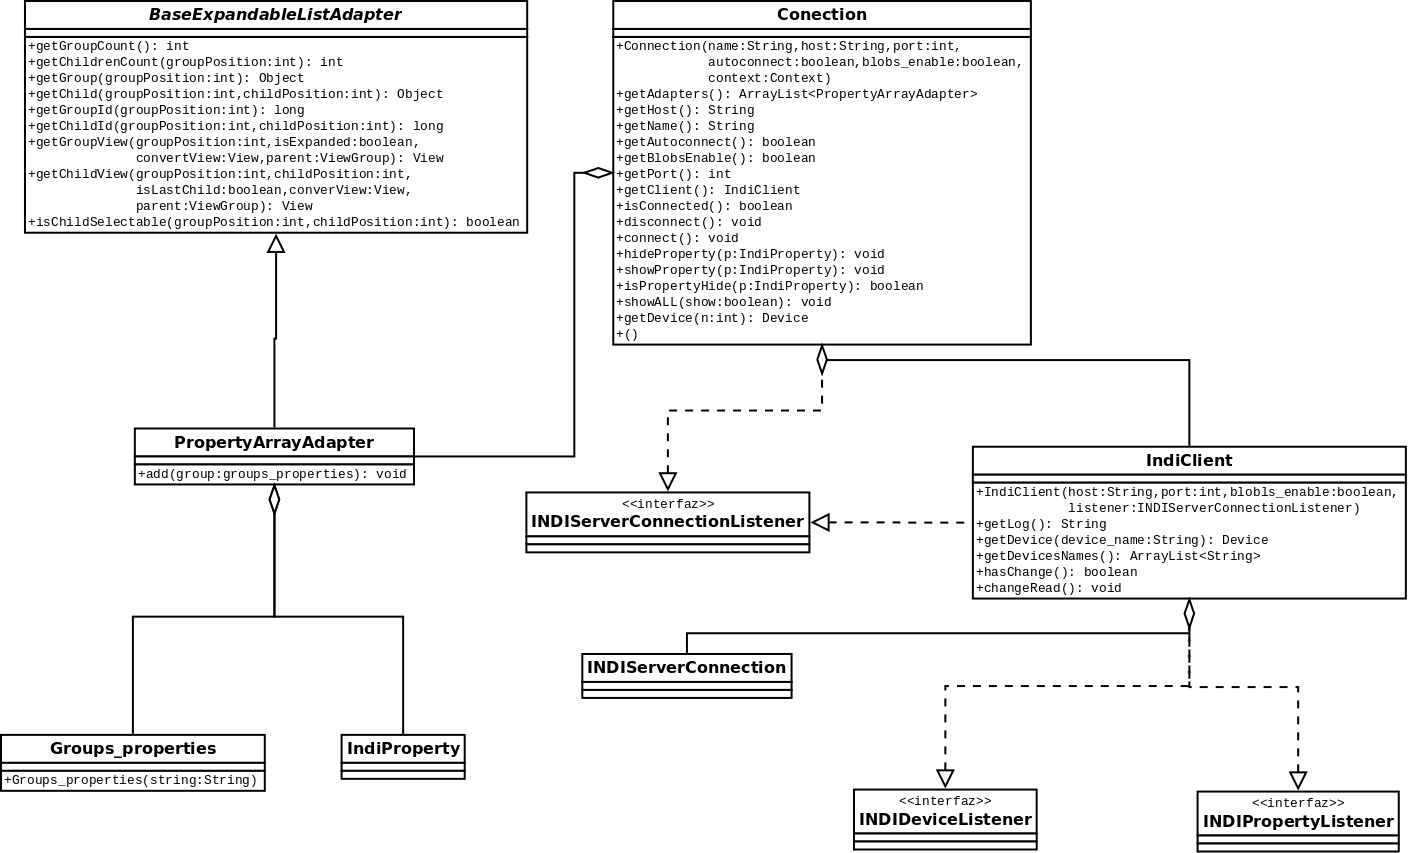
\includegraphics[width=1\textwidth]{../images/indi_diag_clases.png}
  \caption{Diagrama de clases asociadas a INDI}
  \label{fig:diag_indi_clases}
  \end{center}
\end{figure}


\newpage
\subsection{Diseño de las clases manejadoras de propiedades}

Como se explicó en la introducción, \textbf{INDI} maneja 5 tipos de propiedades:


\begin{itemize}
  \item \textbf{Text.}
  \item \textbf{Number.}
  \item \textbf{Switch.}
  \item \textbf{Blob.}
  \item \textbf{Light.}
\end{itemize}

\bigskip
Para manejar cada una de estas propiedades se crea una clase que recibirá un objeto \textit{INDIProperty} (del que heredan todos los tipos) y según el tipo informarán de que pueden manejar dicha propiedad y construirán las interfaces de usuario para mostrarla y editarla.

\bigskip
Gracias a la creación de la interfaz de Java \textit{UIPropertyManager} podemos añadir más manejadores de propiedades. Para ilustrar su uso se han creado dos manejadores más:

\begin{itemize}
  \item \textbf{Connection.}
  \item \textbf{Abort.}
\end{itemize}

\bigskip
Estas dos propiedades son de tipo \textit{Switch} pero tienen la peculiaridad de que siempre tienen la misma estructura: mismo número de elementos, mismo nombre para cada elemento, etc. Por ello podemos analizar la propiedad recibida y ver si es de esos tipos, informando de que podemos manejarla, y construyendo vistas especificas para esas propiedades (como son de tipo \textit{Switch} su vista por defecto sería la de todas las propiedades de este tipo).

\bigskip
En la figura \ref{fig:diag_manager_ui} podemos ver el diagrama de clases que ilustra la creación de los manejadores, implementando las interfaces para manejar propiedades y , adicionalmente, para manejar la pulsación sobre un objeto \textit{View} de Android.

\bigskip
\begin{figure}[!ht]
  \begin{center}
  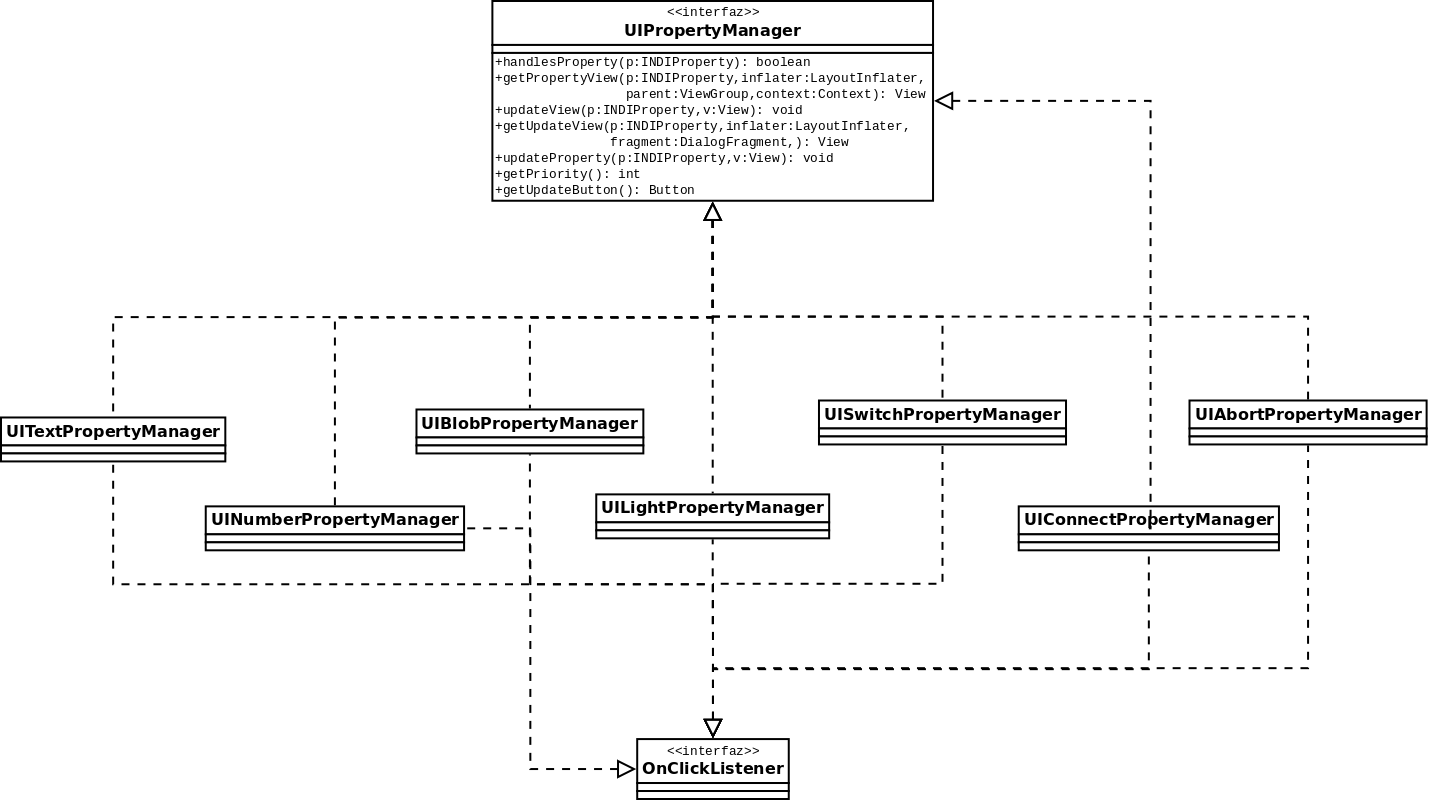
\includegraphics[width=1\textwidth]{../images/manager_ui.png}
  \caption{Diagrama de clases asociadas a los manejadores de propiedades}
  \label{fig:diag_manager_ui}
  \end{center}
\end{figure}

\newpage
\subsection{Diseño de las clases manejadoras de dispositivos}

Finalmente, necesitamos manejar y decidir como mostramos una propiedad y sus elementos. Para implementar esta funcionalidad se ha optado por utilizar los elementos visuales de Android \textit{tabs} que permiten mostrar vistas tabuladas. Con esto, vamos a crear una vista por defecto para cualquier dispositivo. Esta vista es la utilizada en las secciones anteriores: \textit{las listas expandibles de android}.

\bigskip
En la figura \ref{fig:diag_manager_ui_device} podemos ver que tenemos una clase \textit{DefaultDeviceView} que se mostrará por defecto para todas los dispositivos. Este es el comportamiento normal de la aplicación

\bigskip
Siguiente con el objetivo principal de facilitar la extensibilidad para añadir nuevas vistas de dispositivo, se ha diseñado una clase abstracta, \textit{DeviceView}, para facilitar la creación de nuevas vistas. Solo tenemos que crear una clase que herede de esta clase abstracta e implementar los métodos. Al ser una clase que hereda de \textit{Fragment}, dentro de ella tenemos libertad para mostrar las propiedades del dispositivo para personalizarlo. Cada nueva vista sería una tabulación más en la vista tabulada.


\bigskip
\begin{figure}[!ht]
  \begin{center}
  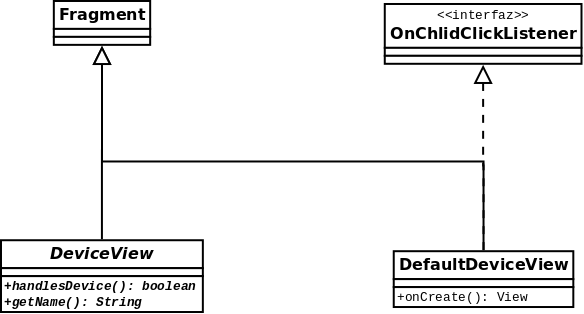
\includegraphics[width=1\textwidth]{../images/device_ui.png}
  \caption{Diagrama de clases asociadas a los manejadores de dispositivos}
  \label{fig:diag_manager_ui_device}
  \end{center}
\end{figure}


\bigskip
\section{Diseño de las interfaces de usuario}

Las interfaces de usuario deben ser objeto de un cuidadoso diseño dado que estamos construyendo una aplicación móvil, y el éxito dependerá en gran medida de una buena interfaz de usuario que sea útil, clara y fácil de usar.

\bigskip
A lo largo del diseño de las interfaces de usuario, se fueron mejorando sucesivamente las distintas vistas desde bocetos en papel (figuras \ref{fig:boceto} y \ref{fig:boceto_2}) hasta primeras versiones ya implementadas en la aplicación (figuras \ref{fig:capturas} y \ref{fig:capturas2}).


\begin{figure}
    \centering
    \begin{subfigure}[]{0.4\textwidth}
        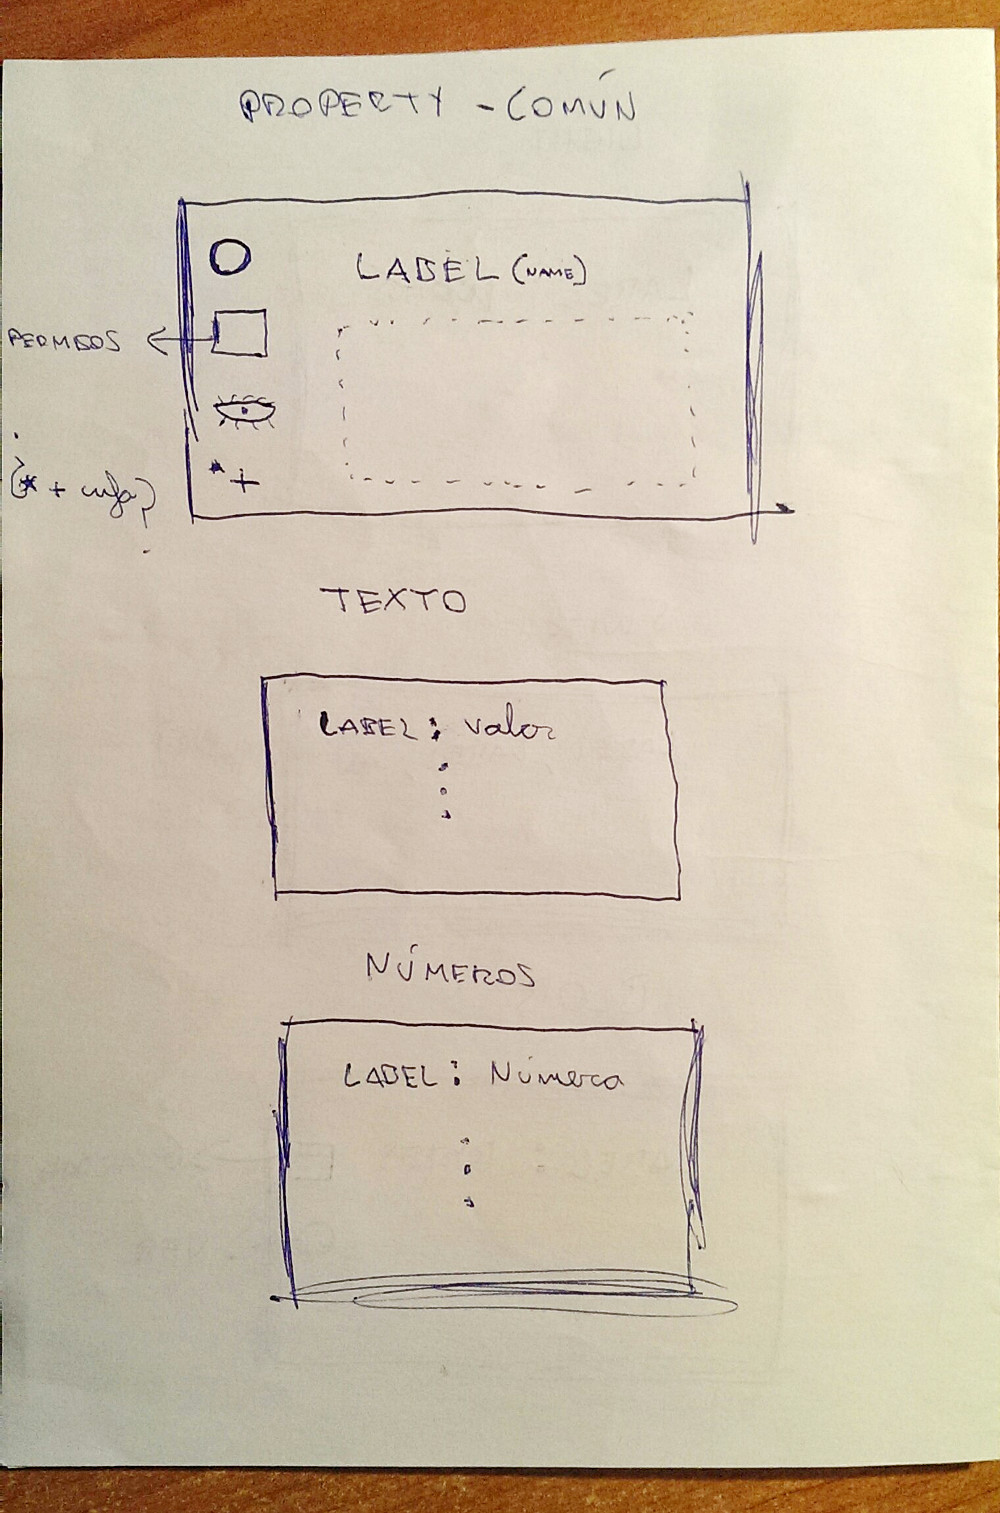
\includegraphics[width=\textwidth]{../images/boceto.jpg}
        \caption{}
        \label{fig:boceto}
    \end{subfigure}
    \begin{subfigure}[]{0.4\textwidth}
        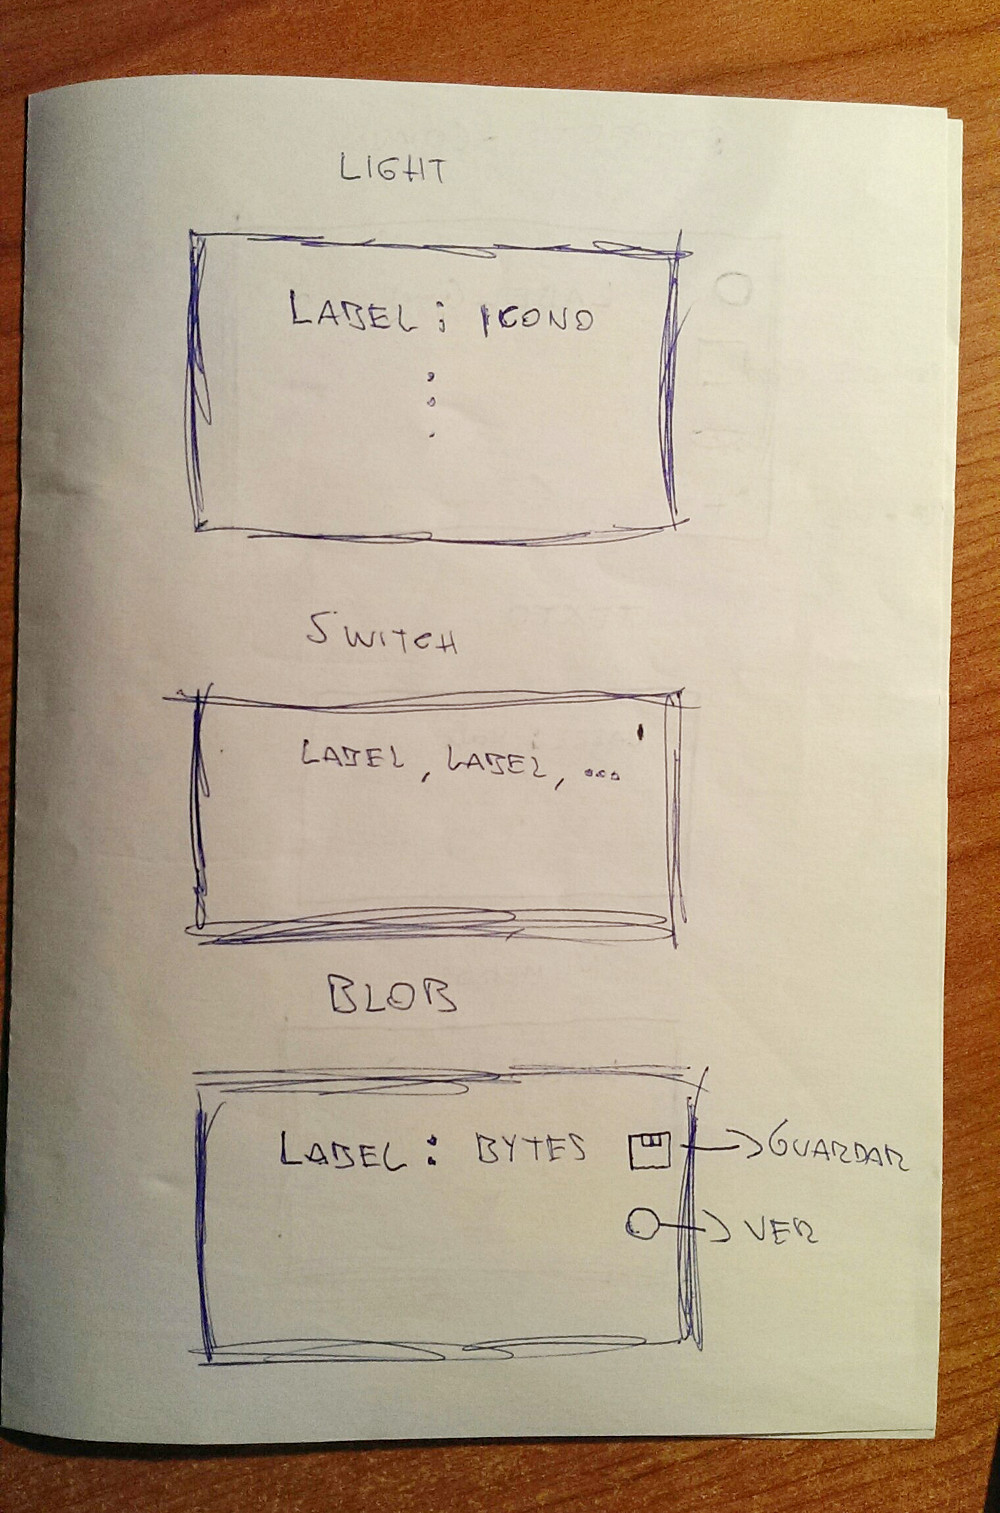
\includegraphics[width=\textwidth]{../images/boceto2.jpg}
        \caption{}
        \label{fig:boceto_2}
    \end{subfigure}
    \caption{Bocetos}\label{fig:bocetos}
\end{figure}

\begin{figure}
    \centering
    \begin{subfigure}[]{0.4\textwidth}
        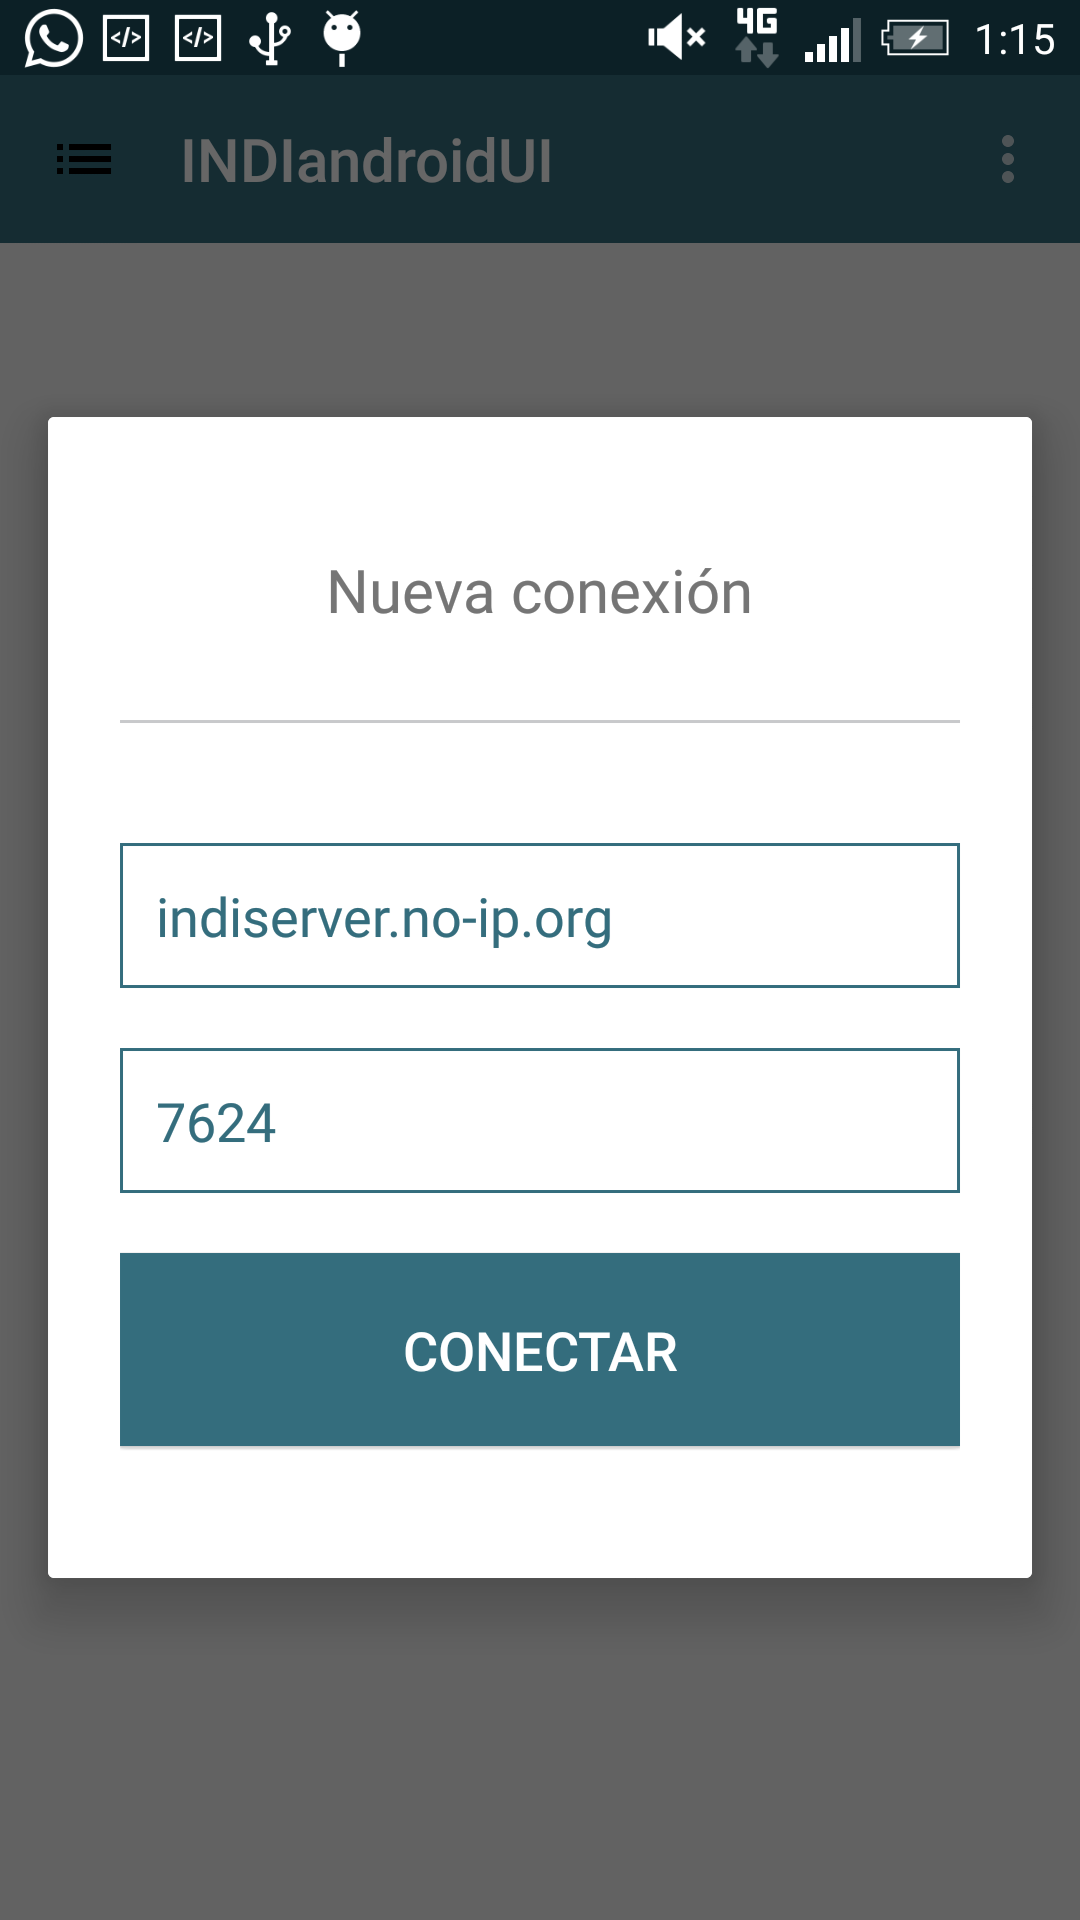
\includegraphics[width=\textwidth]{../images/captura.png}
        \caption{}
        \label{fig:captura1}
    \end{subfigure}
    \begin{subfigure}[]{0.4\textwidth}
        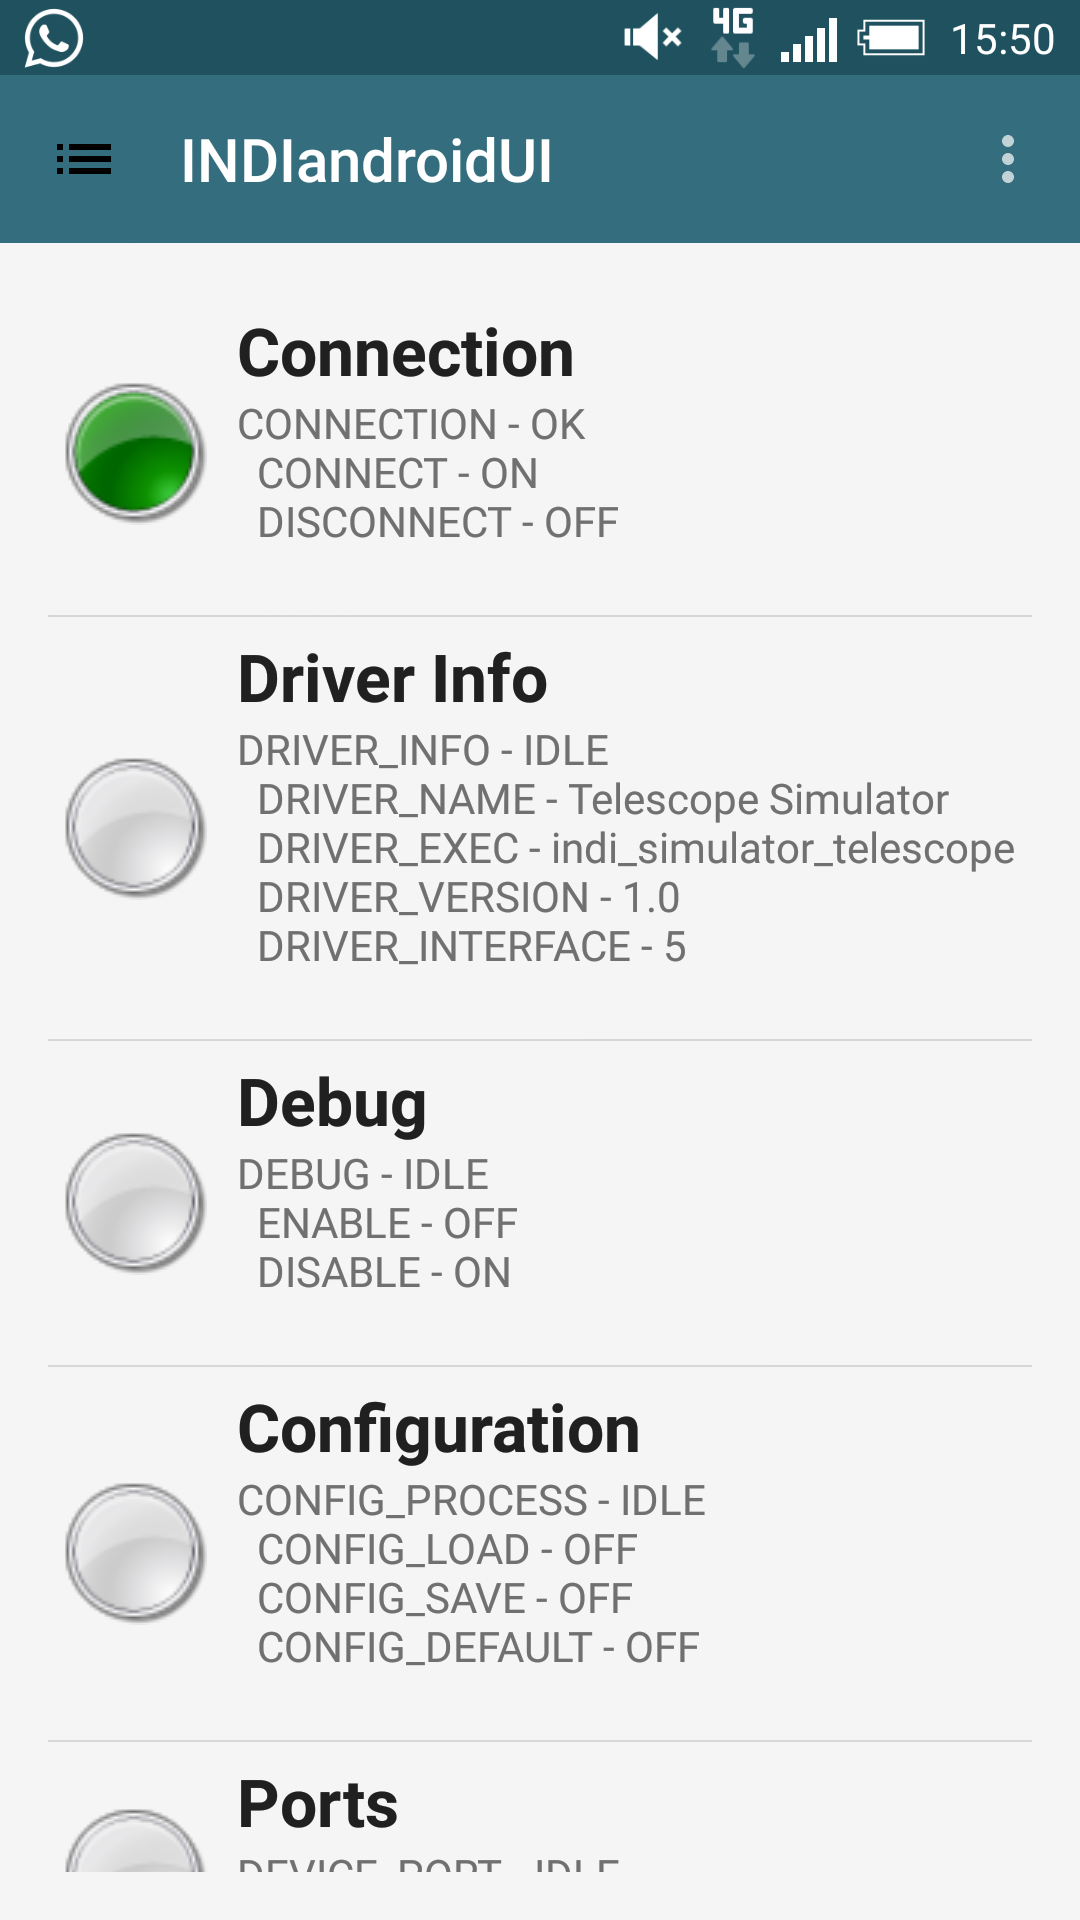
\includegraphics[width=\textwidth]{../images/captura2.png}
        \caption{}
        \label{fig:captura2}
    \end{subfigure}
    \caption{Capturas}\label{fig:capturas}
\end{figure}

\begin{figure}
    \centering
    \begin{subfigure}[]{0.4\textwidth}
        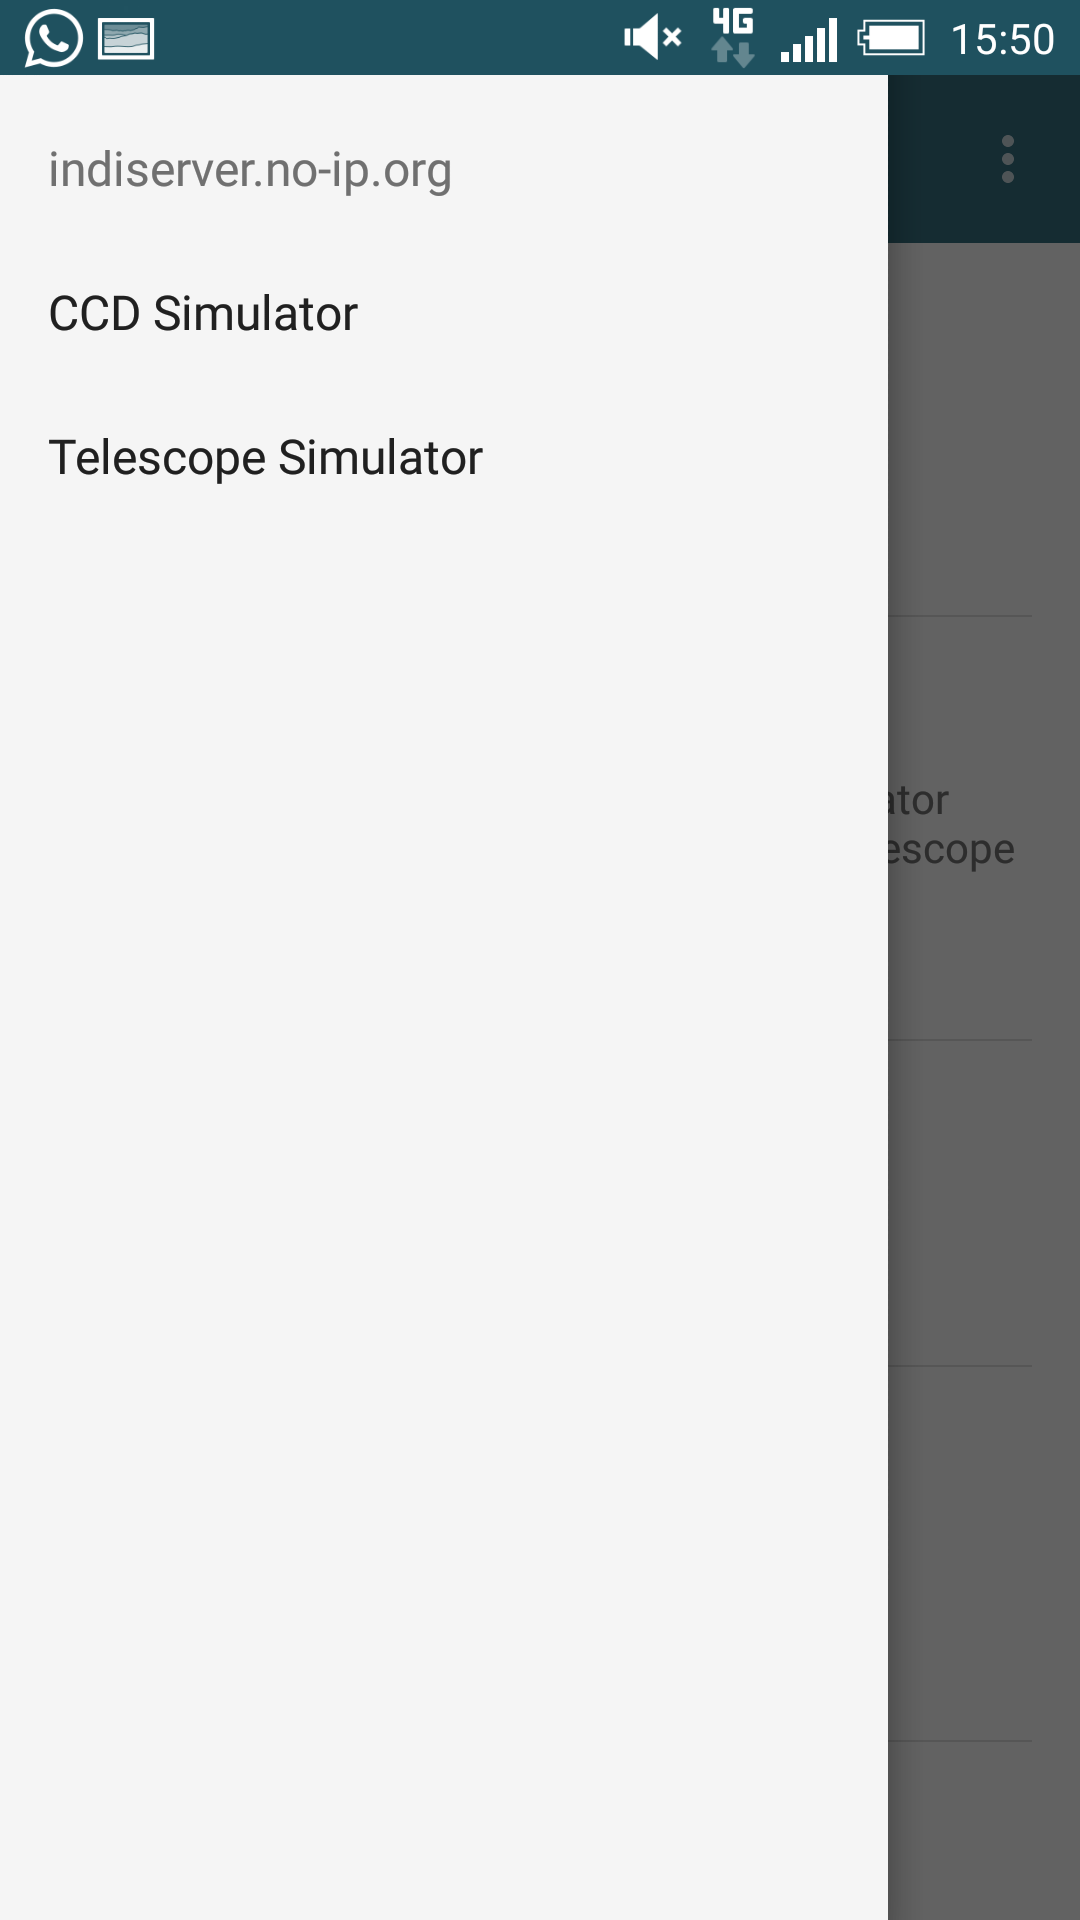
\includegraphics[width=\textwidth]{../images/captura3.png}
        \caption{}
        \label{fig:captura3}
    \end{subfigure}
    \begin{subfigure}[]{0.4\textwidth}
        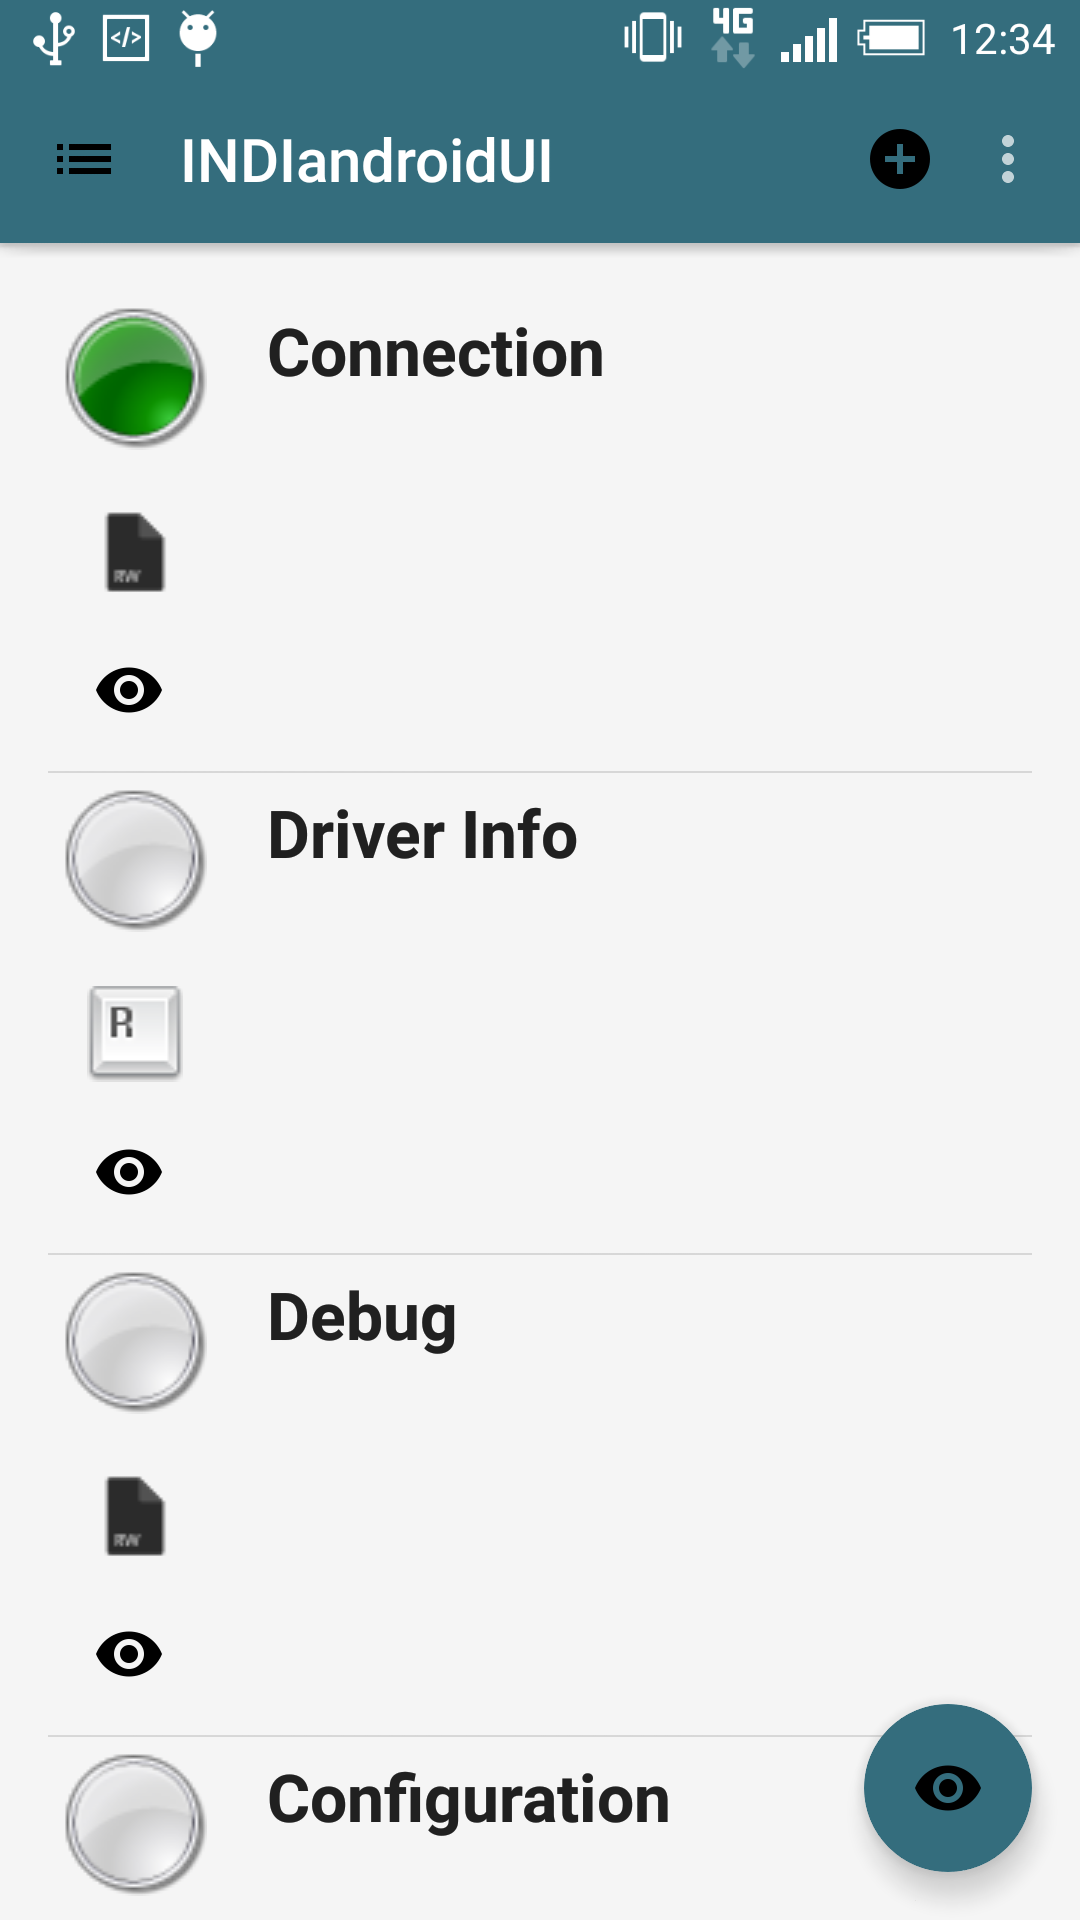
\includegraphics[width=\textwidth]{../images/captura5.png}
        \caption{}
        \label{fig:captura4}
    \end{subfigure}
    \caption{Capturas}\label{fig:capturas2}
\end{figure}

\bigskip
En cada una de las iteraciones del proceso \textbf{Scrum} se fueron rediseñando y mejorando las interfaces de usuario hasta llega a las vistas finales descritas en los siguientes apartados.

\bigskip
Para poder abordar mejor el diseño, se han separados las interfaces en los siguientes grupos:

\begin{itemize}
  \item \textbf{Interfaz principal de la aplicación.}
  \item \textbf{Interfaz para listar las propiedades.}
  \item \textbf{Interfaz de propiedad.}
  \item \textbf{Interfaz de diálogos}
  \item \textbf{Interfaz del log}
  \item \textbf{Interfaz de los ajustes}
\end{itemize}

\bigskip
\subsection{Interfaz principal de la aplicación}

La interfaz principal es la más importante de cara al usuario. Define como se va a organizar toda la información y la navegabilidad dentro de la aplicación. 

\bigskip
En cada iteración se han añadido nuevas funcionalidades a la aplicación lo cual provocaba tener que definir aspectos de la interfaz de usuario principal. 

\bigskip
Por otro lado, en un esfuerzo por seguir las directrices de \textbf{Android} y las tendencias actuales en las aplicaciones móviles, se han incorporado los elementos más actuales tales como la barra de navegación lateral con estilo \textit{material desing} o tener vistas tabuladas. En las figuras \ref{fig:capturas3} y \ref{fig:capturas4} podemos ver la interfaz principal de la aplicación.

\begin{figure}
    \centering
    \begin{subfigure}[]{0.4\textwidth}
        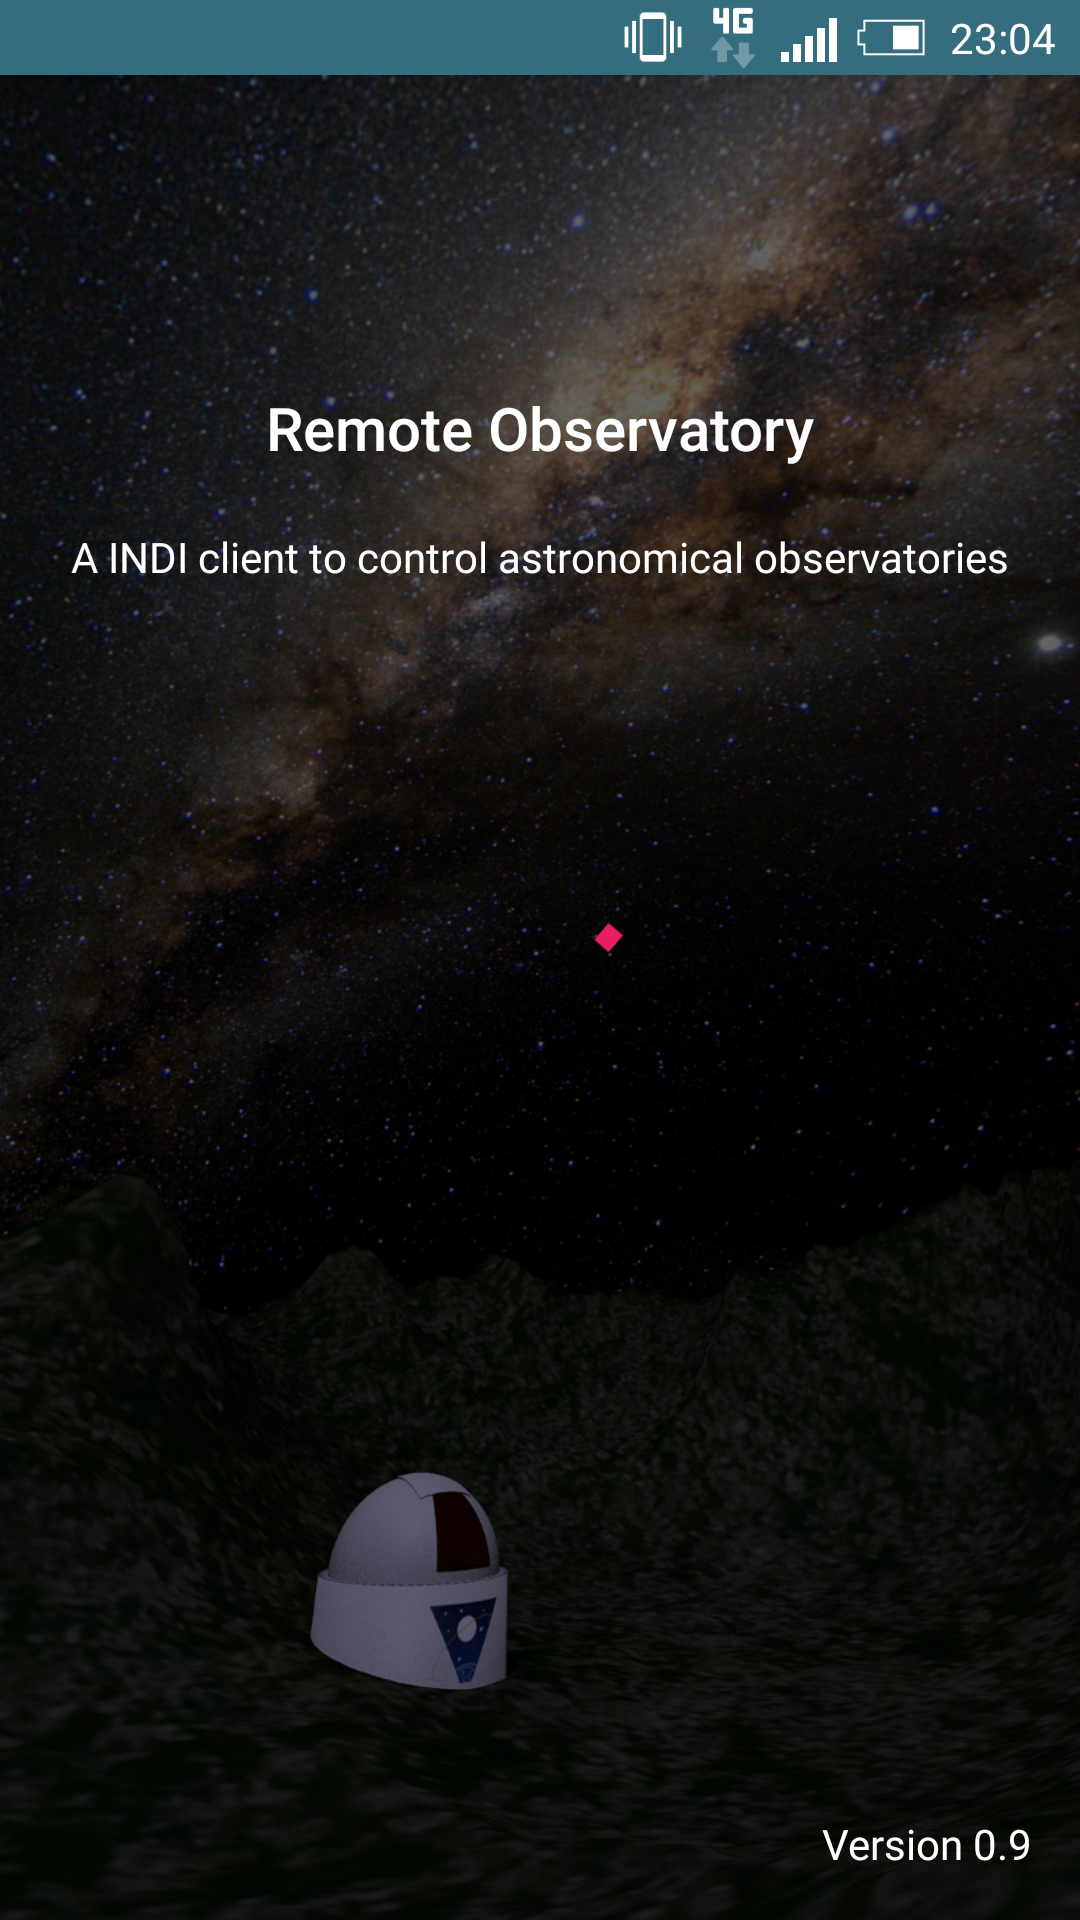
\includegraphics[width=\textwidth]{../images/captura6.png}
        \caption{}
        \label{fig:captura4}
    \end{subfigure}
    \begin{subfigure}[]{0.4\textwidth}
        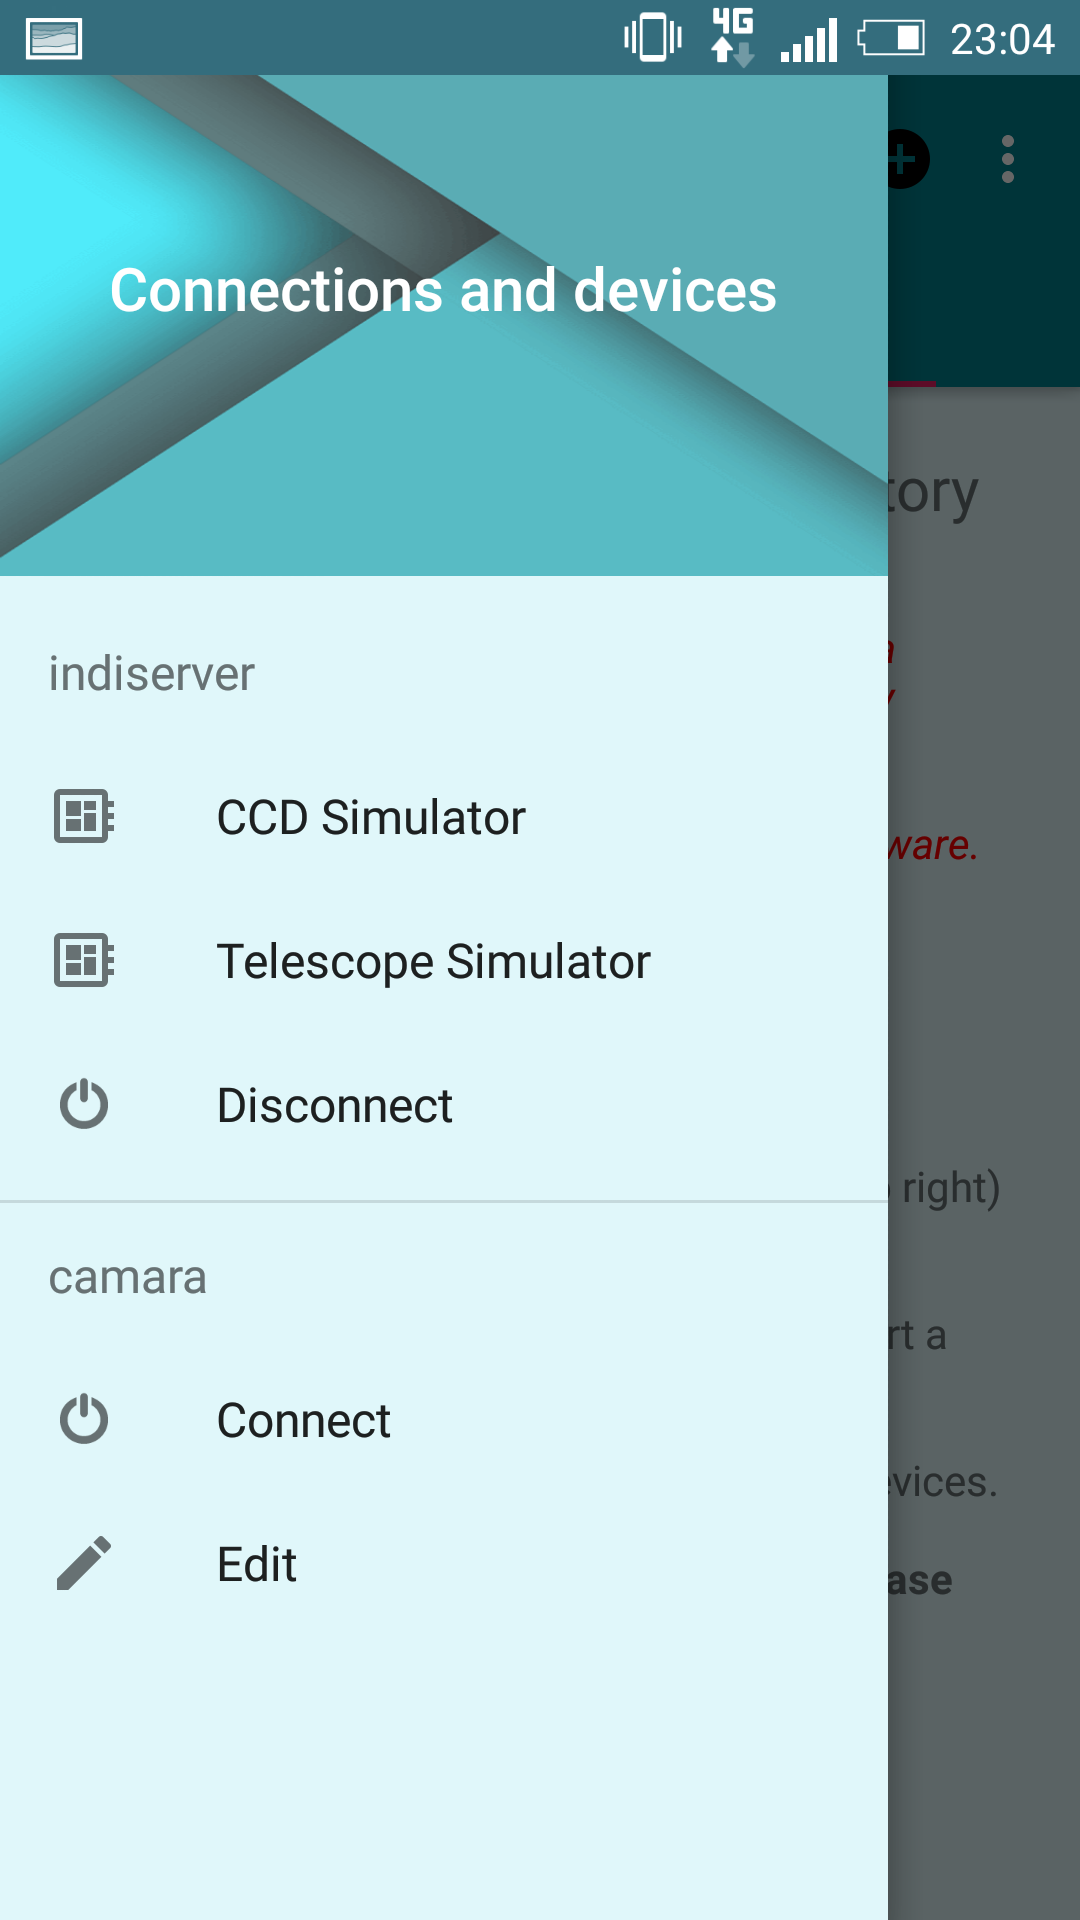
\includegraphics[width=\textwidth]{../images/captura7.png}
        \caption{}
        \label{fig:captura5}
    \end{subfigure}
    \caption{Capturas de la interfaz principal}\label{fig:capturas3}
\end{figure}

\begin{figure}
    \centering
    \begin{subfigure}[]{0.4\textwidth}
        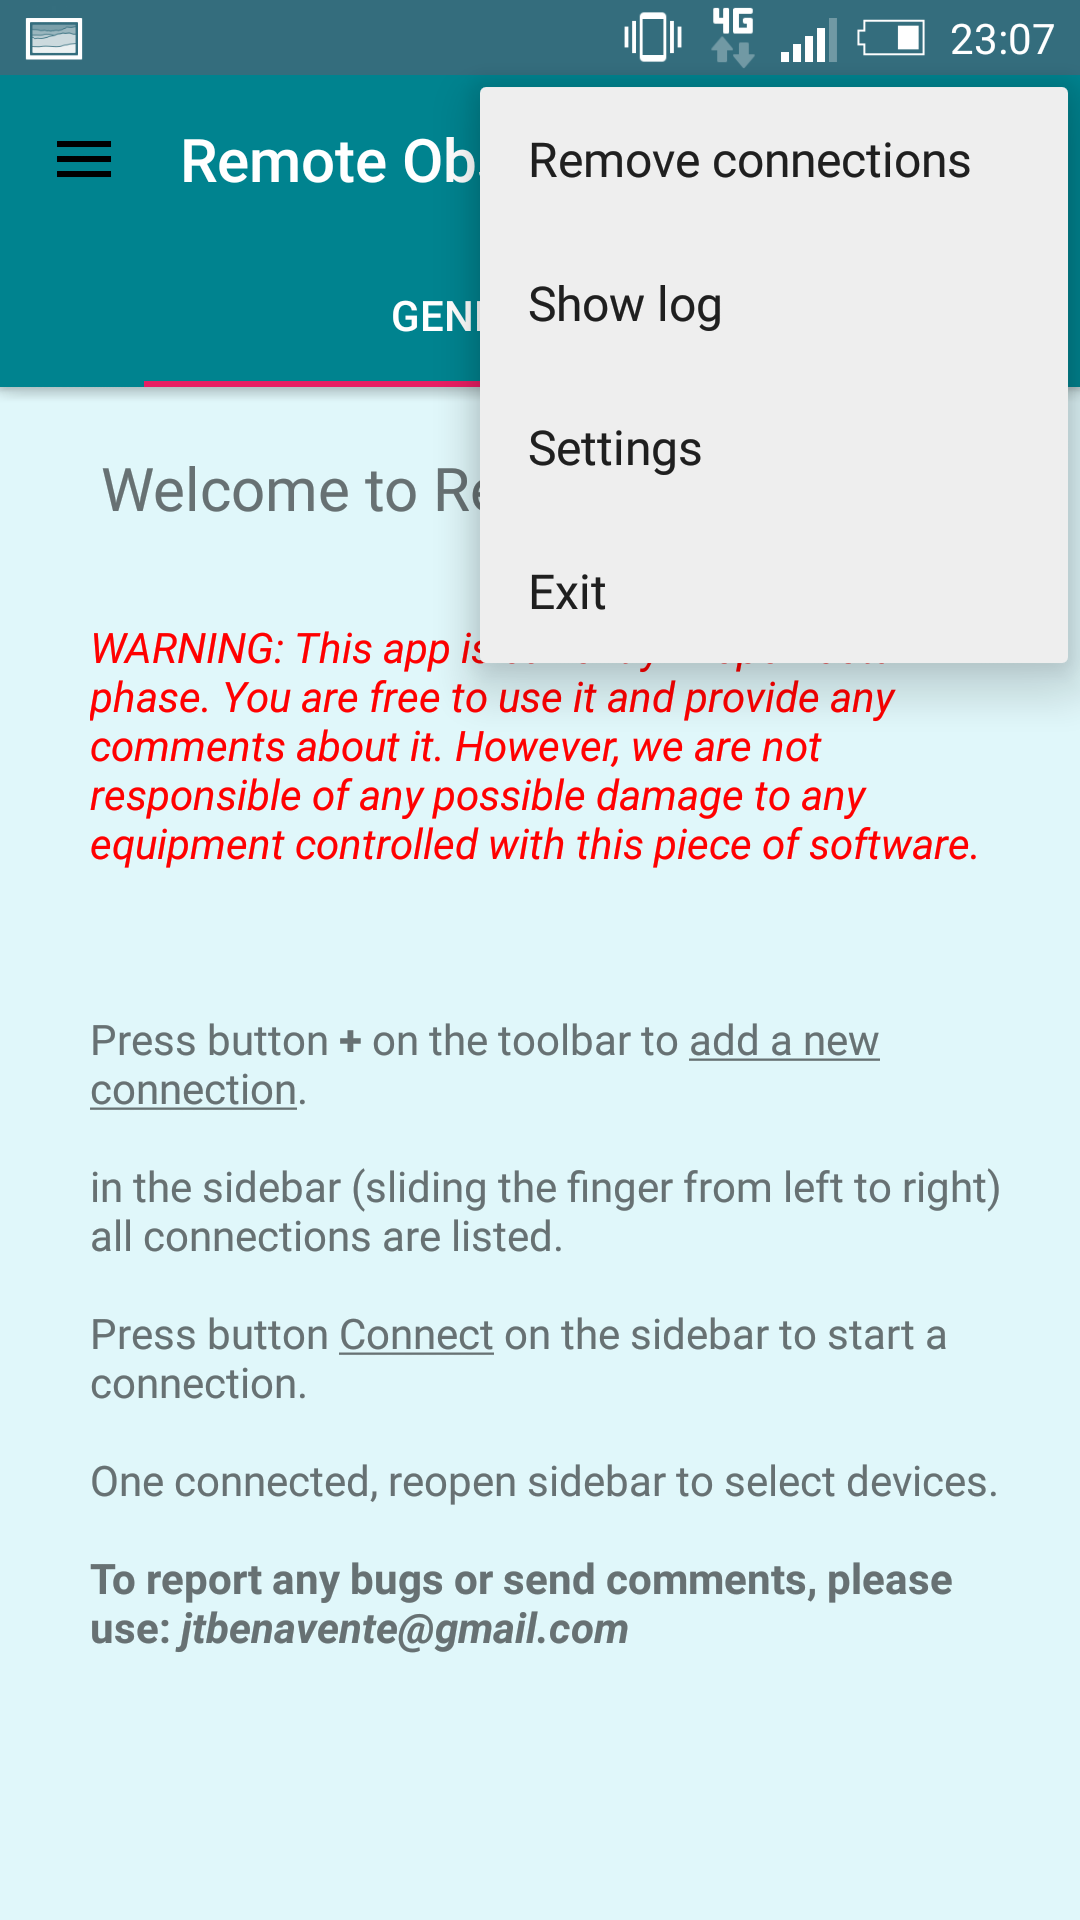
\includegraphics[width=\textwidth]{../images/captura8.png}
        \caption{}
        \label{fig:captura6}
    \end{subfigure}
    \begin{subfigure}[]{0.4\textwidth}
        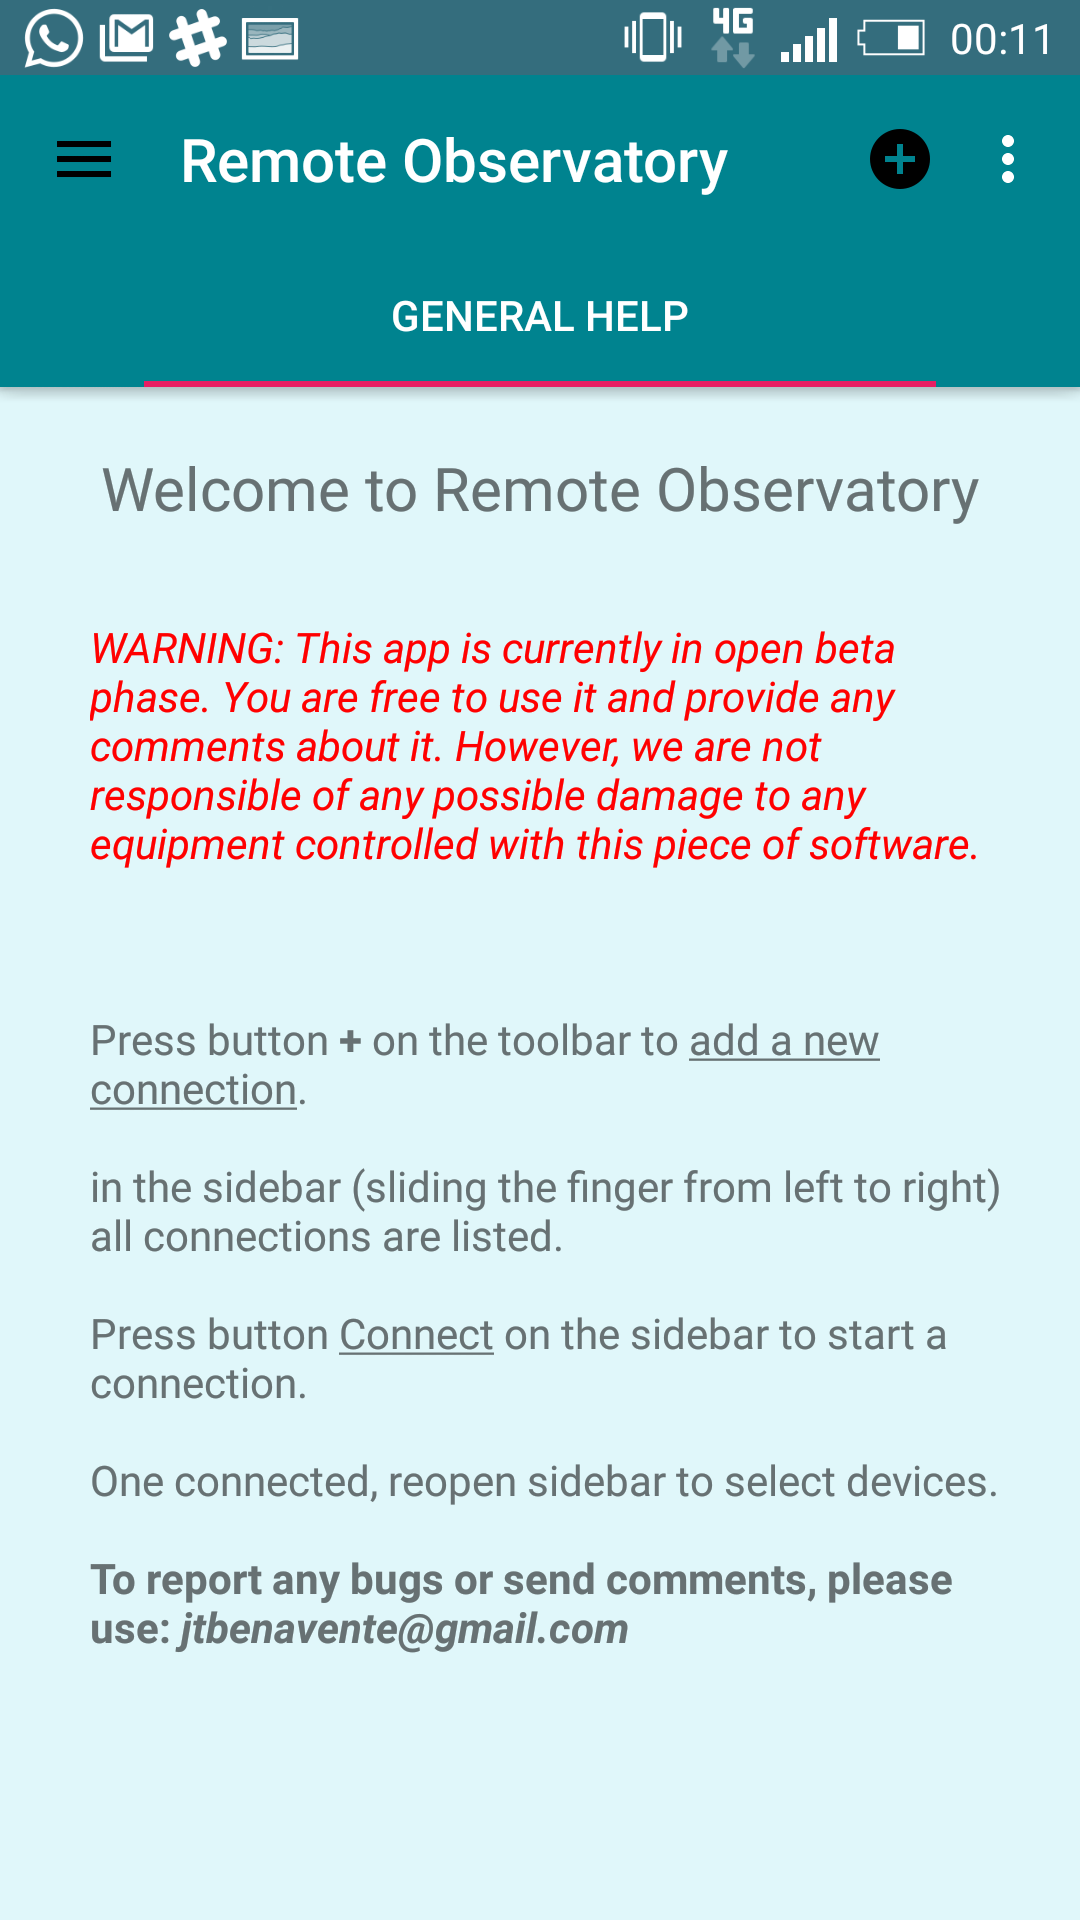
\includegraphics[width=\textwidth]{../images/captura9.png}
        \caption{}
        \label{fig:captura7}
    \end{subfigure}
    \caption{Capturas de la interfaz principal}\label{fig:capturas4}
\end{figure}


\bigskip
\subsection{Interfaz para listar las propiedades}

Una vez definido el aspecto general de la aplicación y los modos de navegación, el principal objetivo es poder listar las propiedades de los dispositivos. Desde las primeras reunión tuvimos claro que debíamos usar una lista estándar de \textbf{Android}, aunque debíamos abordar un tema importante: la posibilidad de agrupar las propiedades de un mismo grupo.
Hasta la \textbf{cuarta iteración} no se decidió utilizar la que a la postre sería la solución definitiva, \textbf{las listas expandibles}.

\begin{figure}
    \centering
    \begin{subfigure}[]{0.4\textwidth}
        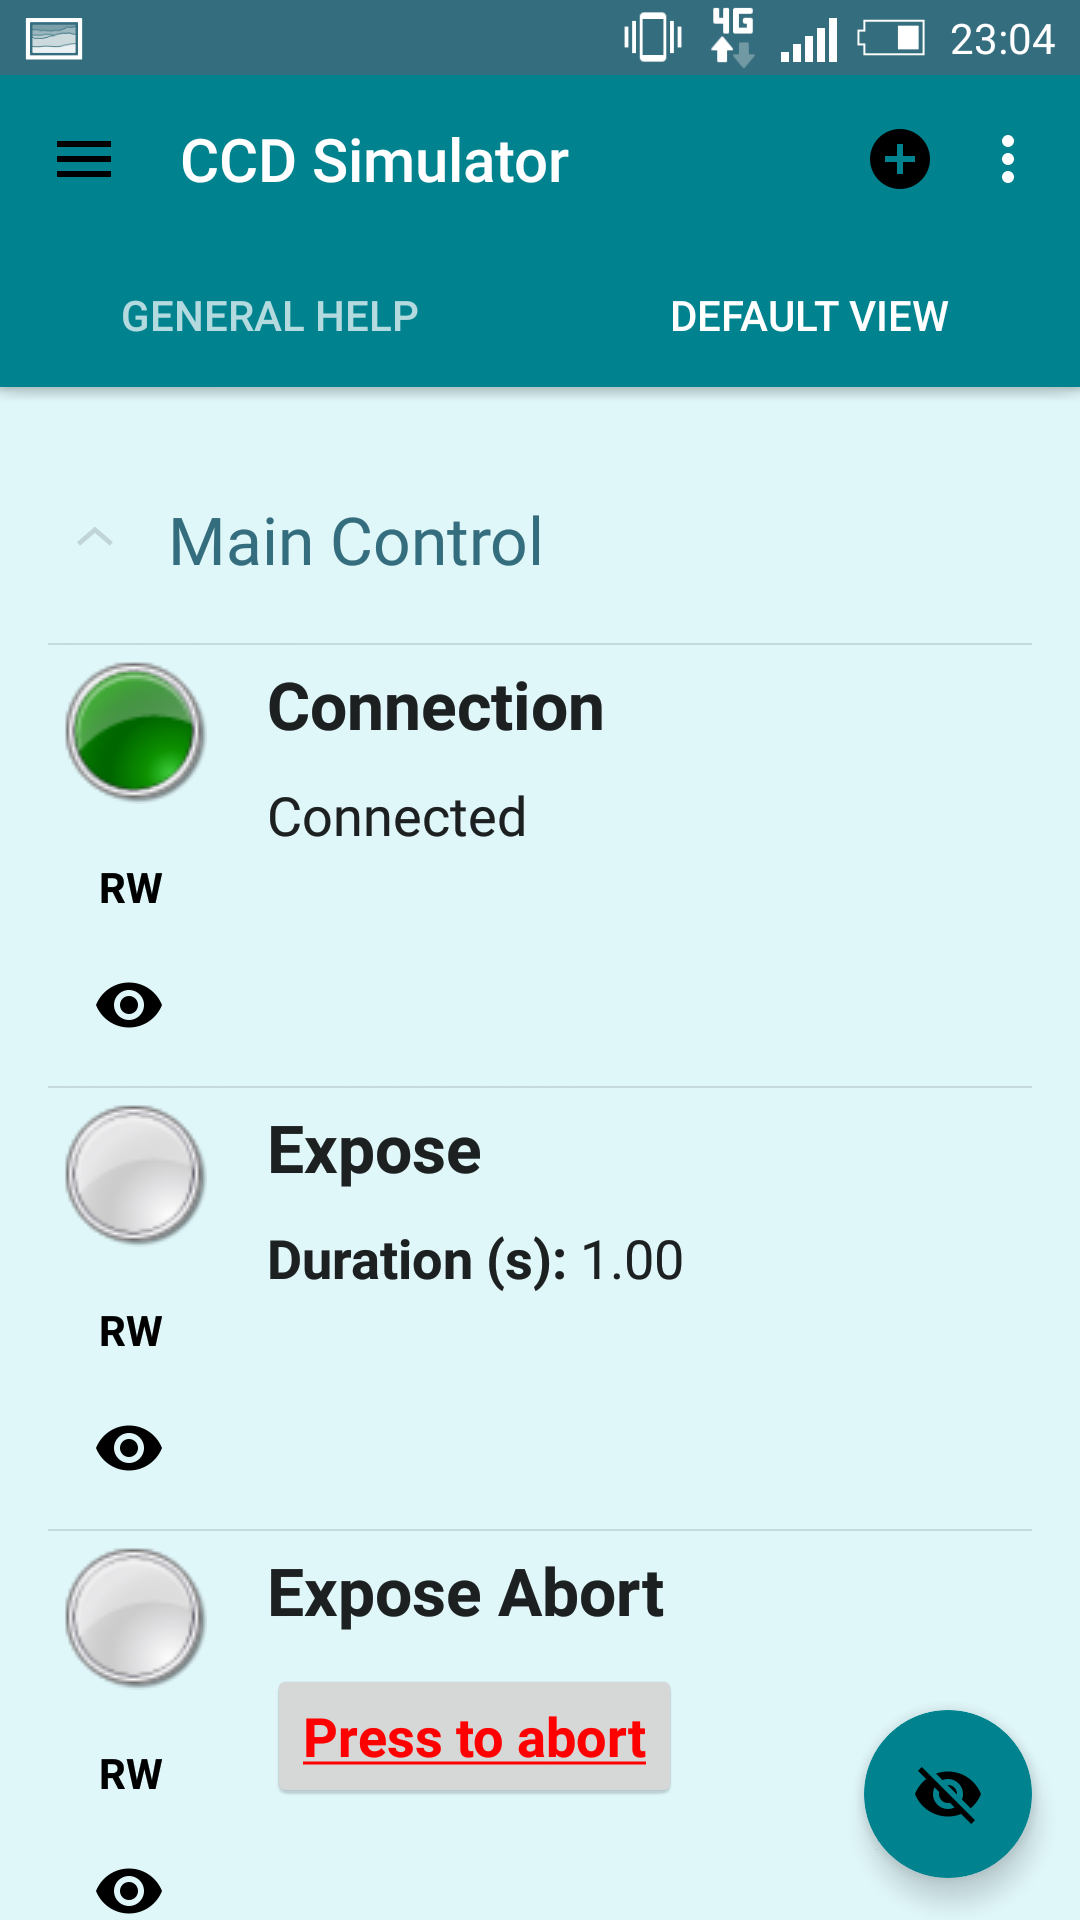
\includegraphics[width=\textwidth]{../images/captura10.png}
        \caption{}
        \label{fig:captura8}
    \end{subfigure}
    \begin{subfigure}[]{0.4\textwidth}
        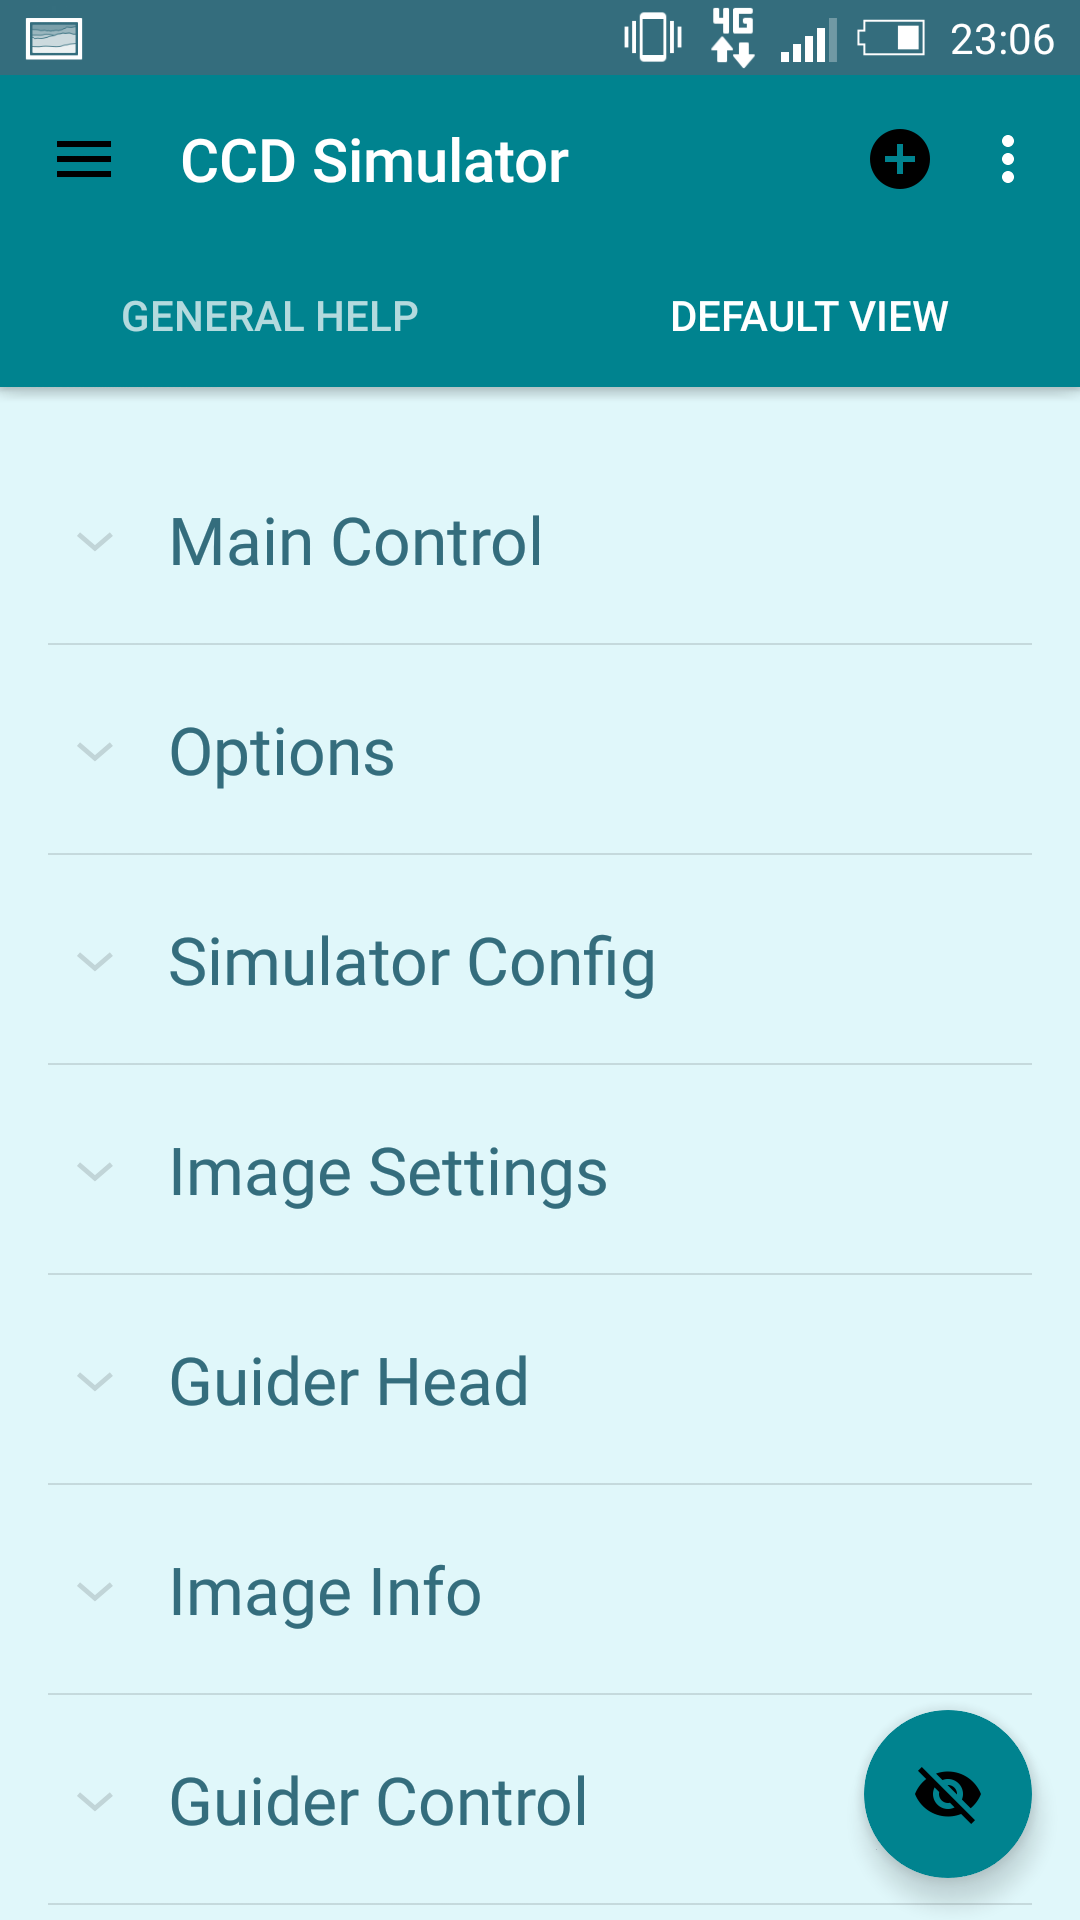
\includegraphics[width=\textwidth]{../images/captura11.png}
        \caption{}
        \label{fig:captura9}
    \end{subfigure}
    \caption{Lista de propiedades de un dispositivo}\label{fig:capturas5}
\end{figure}

En la figura \ref{fig:capturas5} podemos ver las listas con los grupos contraídos y extendidos. Además podemos ver como, en un nuevo esfuerzo por seguir las tendencias más actuales, se ha añadido un \textbf{botón flotante}\cite{ATMFAB} para mostrar u ocultar las propiedades con visibilidad ``oculta''.


\bigskip
\subsection{Interfaz de propiedad}
Una vez definida la lista de las propiedades, abordamos el problema de la interfaz para una propiedad. Para ello analizamos todos los elementos en común y todas las diferencias entre los distintos tipos de propiedades. En la figura \ref{fig:captura4} podemos ver la parte común a todas las propiedades:

\begin{itemize}
  \item \textbf{Nombre de la propiedad.}
  \item \textbf{Estado de la propiedad.}
  \item \textbf{Permisos de escritura y/o lectura.}
  \item \textbf{Visibilidad.}
\end{itemize}

Todas las propiedades comparten estos cuatro elementos, siendo la parte central de la vista la que se adaptará según el tipo.

\bigskip
\subsubsection{Text, Number y Switch}

De cara a los items de la lista, las propiedades \textit{text y number} son idénticas salvo que el valor de los elementos del primero son texto y del segundo son números. Cada elemento se coloca debajo del anterior creando otra lista (una propiedad puede tener uno o más elementos).

En la figura \ref{fig:capturas6} podemos ver ambas vistas en la interfaz de las propiedades. 


\begin{figure}
    \centering
    \begin{subfigure}[]{0.4\textwidth}
        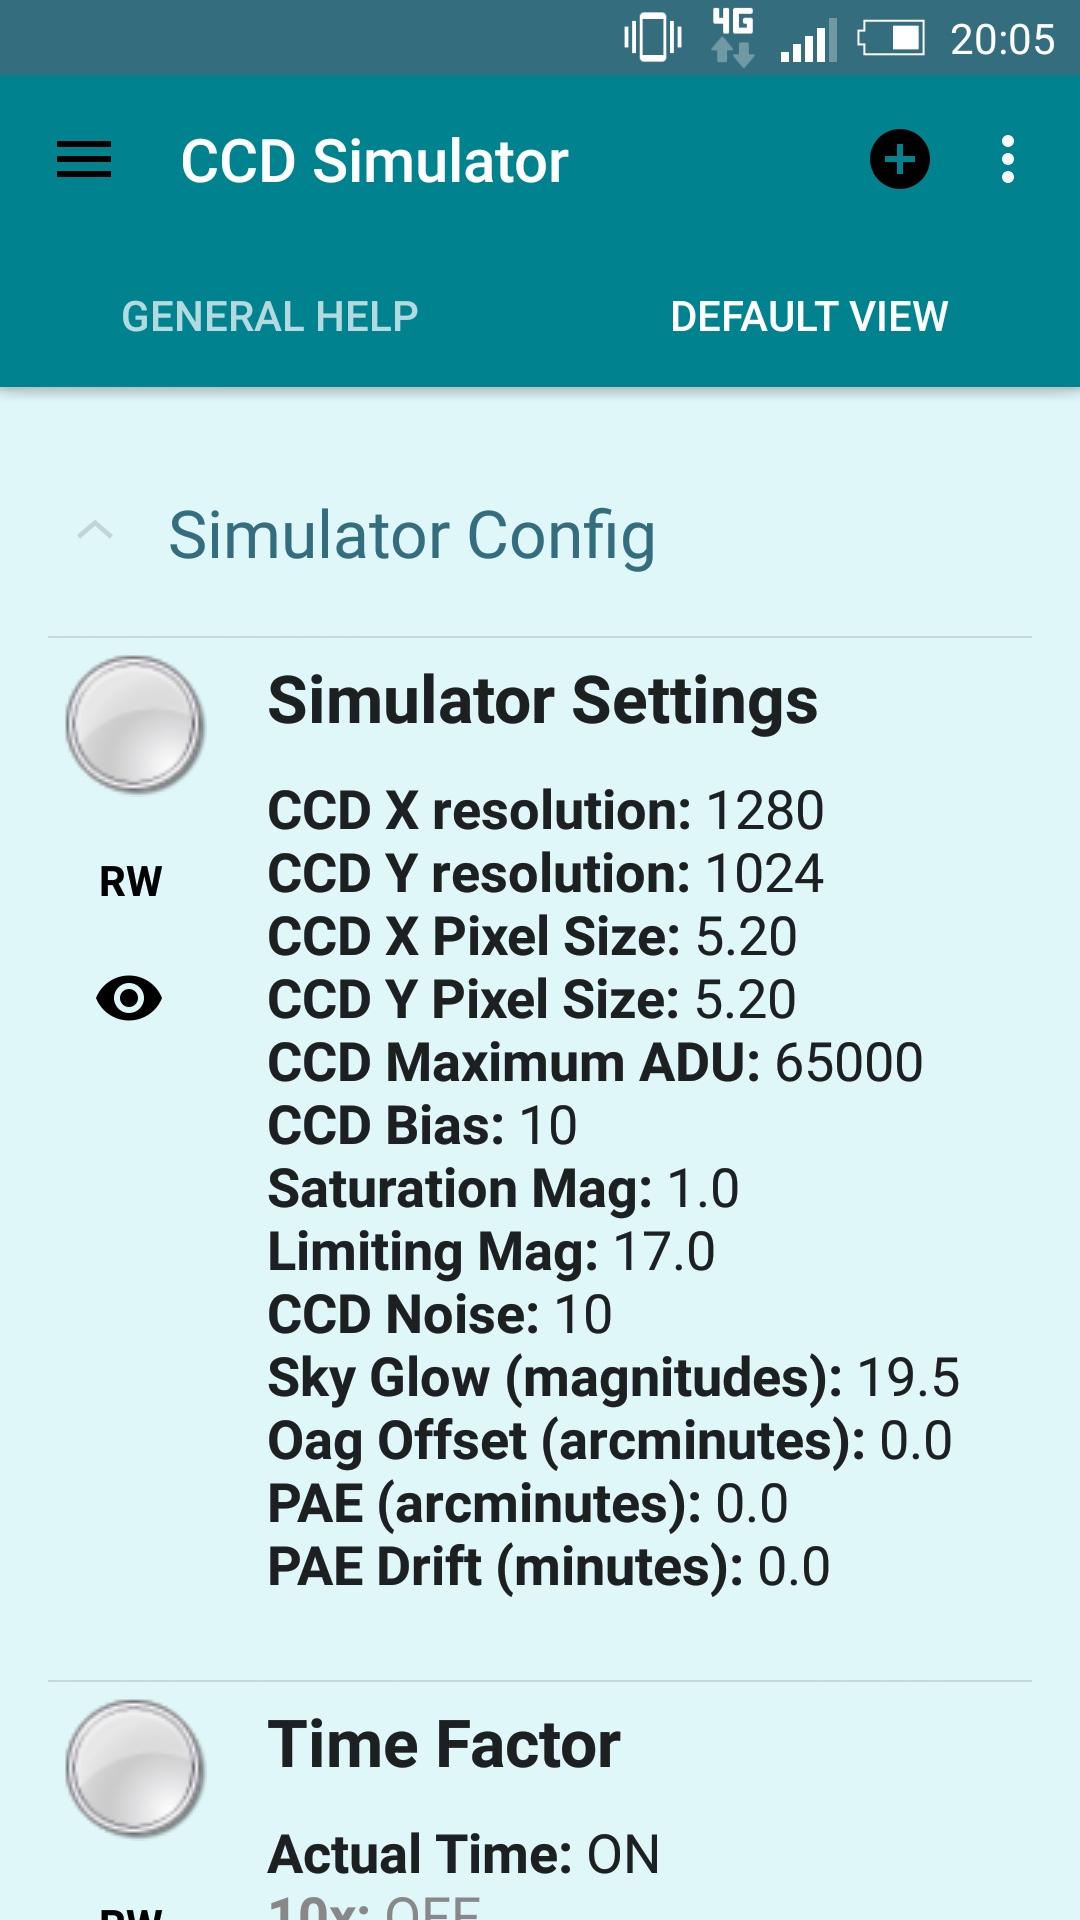
\includegraphics[width=\textwidth]{../images/captura12.png}
        \caption{}
        \label{fig:captura10}
    \end{subfigure}
    \begin{subfigure}[]{0.4\textwidth}
        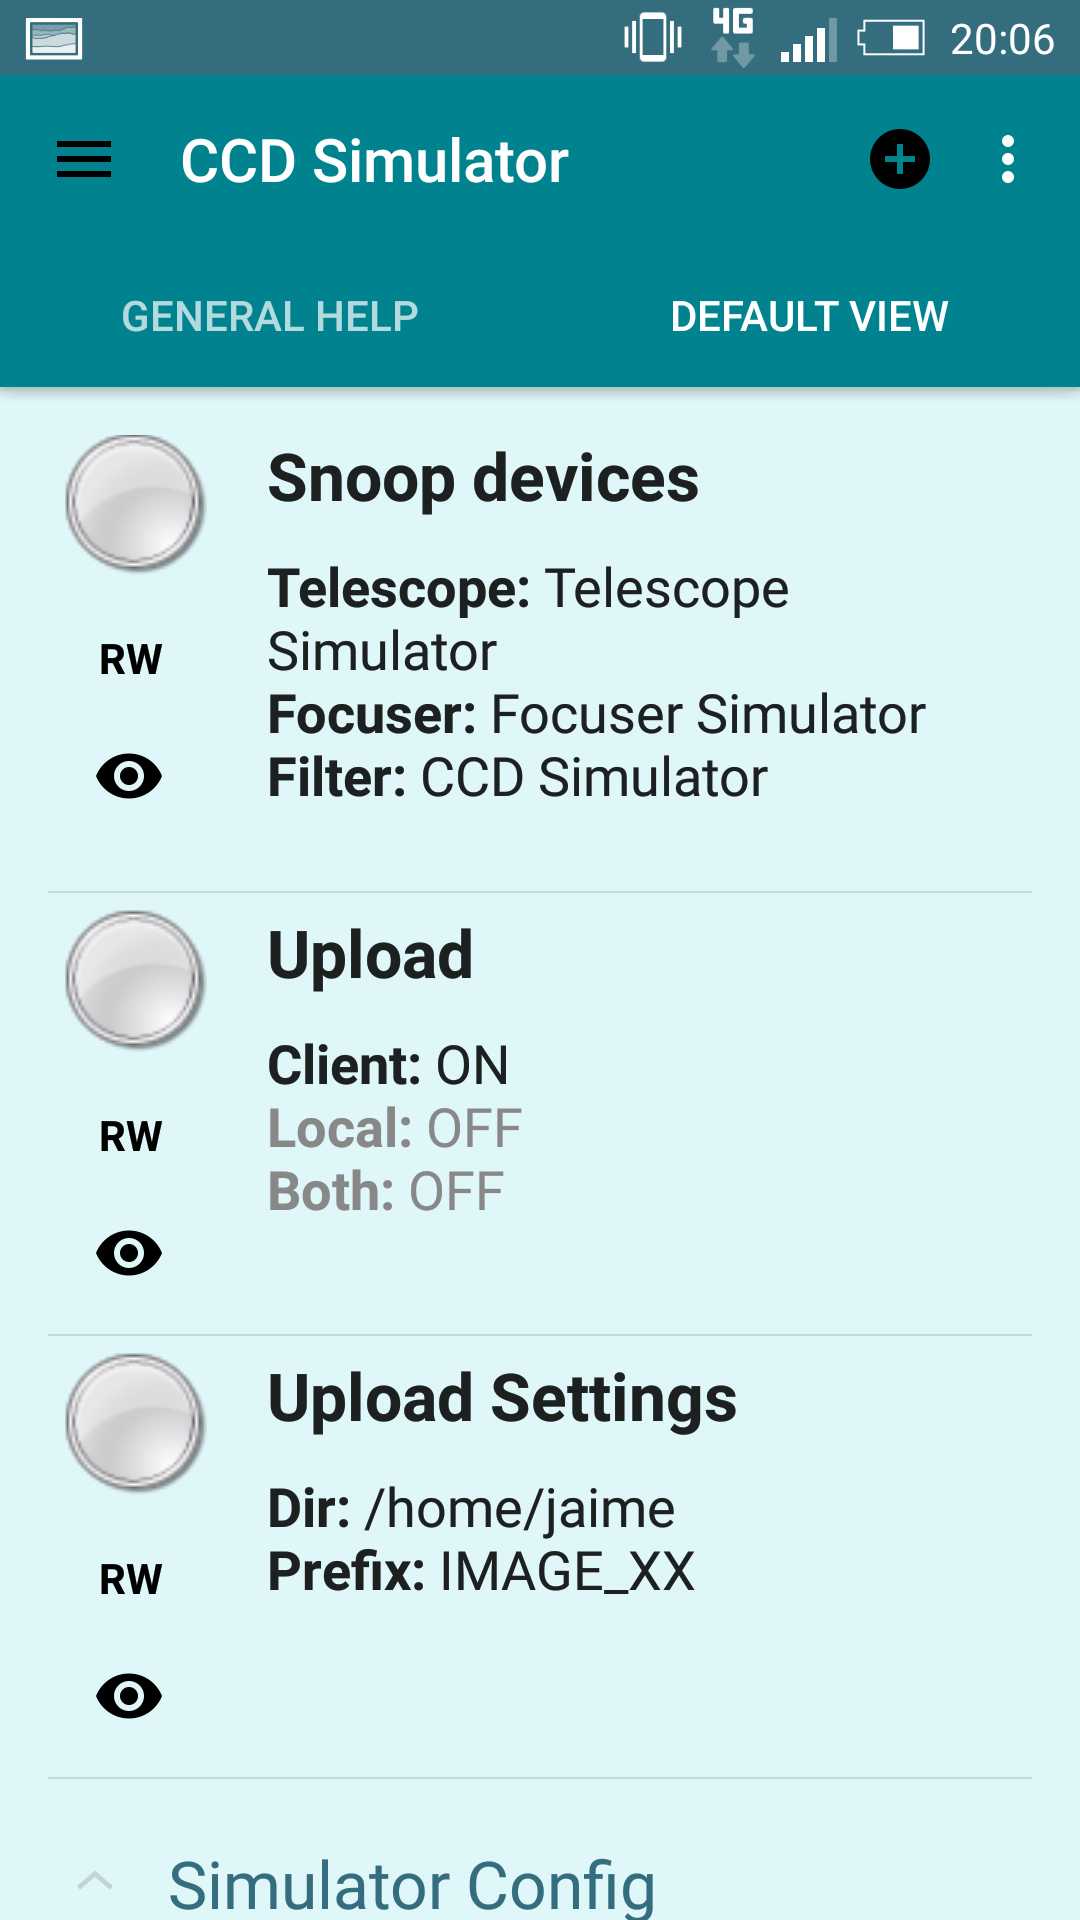
\includegraphics[width=\textwidth]{../images/captura13.png}
        \caption{}
        \label{fig:captura11}
    \end{subfigure}
    \caption{Propiedades text, number y switch}\label{fig:capturas6}
\end{figure}

Los \textit{Switch} tienen una vista similar a las dos propiedades anteriores, salvo que el valor que está en estado ``on'' en negro y los que están en estado ``off'' en gris (figura \ref{fig:capturas6}).


\bigskip
\subsubsection{Blobs}
Los \textit{Switch} son ficheros enviados por el servidor por lo que es más interesante mostrar el tipo de archivo que recibimos y su tamaño. Como se puede ver en la figura \ref{fig:blob}, además de estos dos datos tenemos los botones para poder guardarlo o enviarlo a \textbf{Android} para poder abrirlo con la aplicación adecuada.

\bigskip
\begin{figure}[!ht]
  \begin{center}
  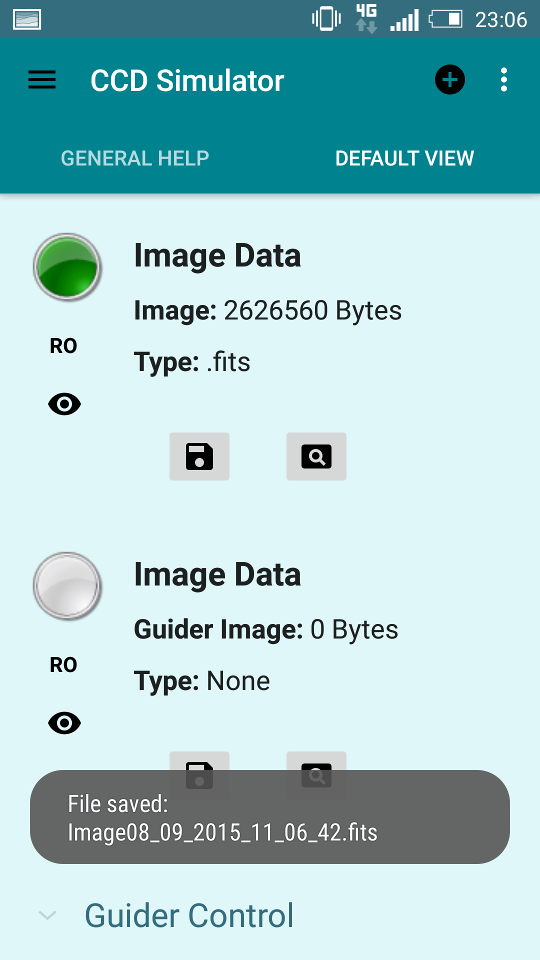
\includegraphics[width=0.3\textwidth]{../images/saveBlob2.png}
  \caption{Vista de un Blob}
  \label{fig:blob}
  \end{center}
\end{figure}

\bigskip
\subsubsection{Light}
Esta propiedad es muy similar a los \textit{switch} salvo que el valor de cada uno de los elementos de la propiedad será un icono representando una luz roja, verde, gris o amarilla.


\bigskip
\subsection{Interfaz de diálogos}

Los diálogos son una herramienta visual esencial que permiten superponer una vista para llamar la atención del usuario, bien sea para informar o para ejecutar alguna acción como editar propiedades.


\bigskip
\subsubsection{Diálagas para editar propiedades}

Estos diálogos permiten editar los elementos de aquellas propiedades que lo permitan:

\begin{itemize}
  \item \textbf{Dialogo de edición de una propiedad Text:} Se muestra la lista de elementos con su \textit{label} y su valor en un cuadro editable (\ref{fig:text_edit}).
  \item \textbf{Dialogo de edición de una propiedad Number:} Se muestra la lista de elementos con su \textit{label} y sus valores máximos y mínimos. Debajo se puede ver el campo editable con el valor (\ref{fig:number_edit}).
  \item \textbf{Dialogo de edición de una propiedad Switch:} Se muestra cada elemento con su \textit{label} seguido de un botón de estados para indicar si el elemento está activo (``on'') o no (``off'') (\ref{fig:number_edit}) .
\end{itemize}


\begin{figure}[!ht]
  \begin{center}
  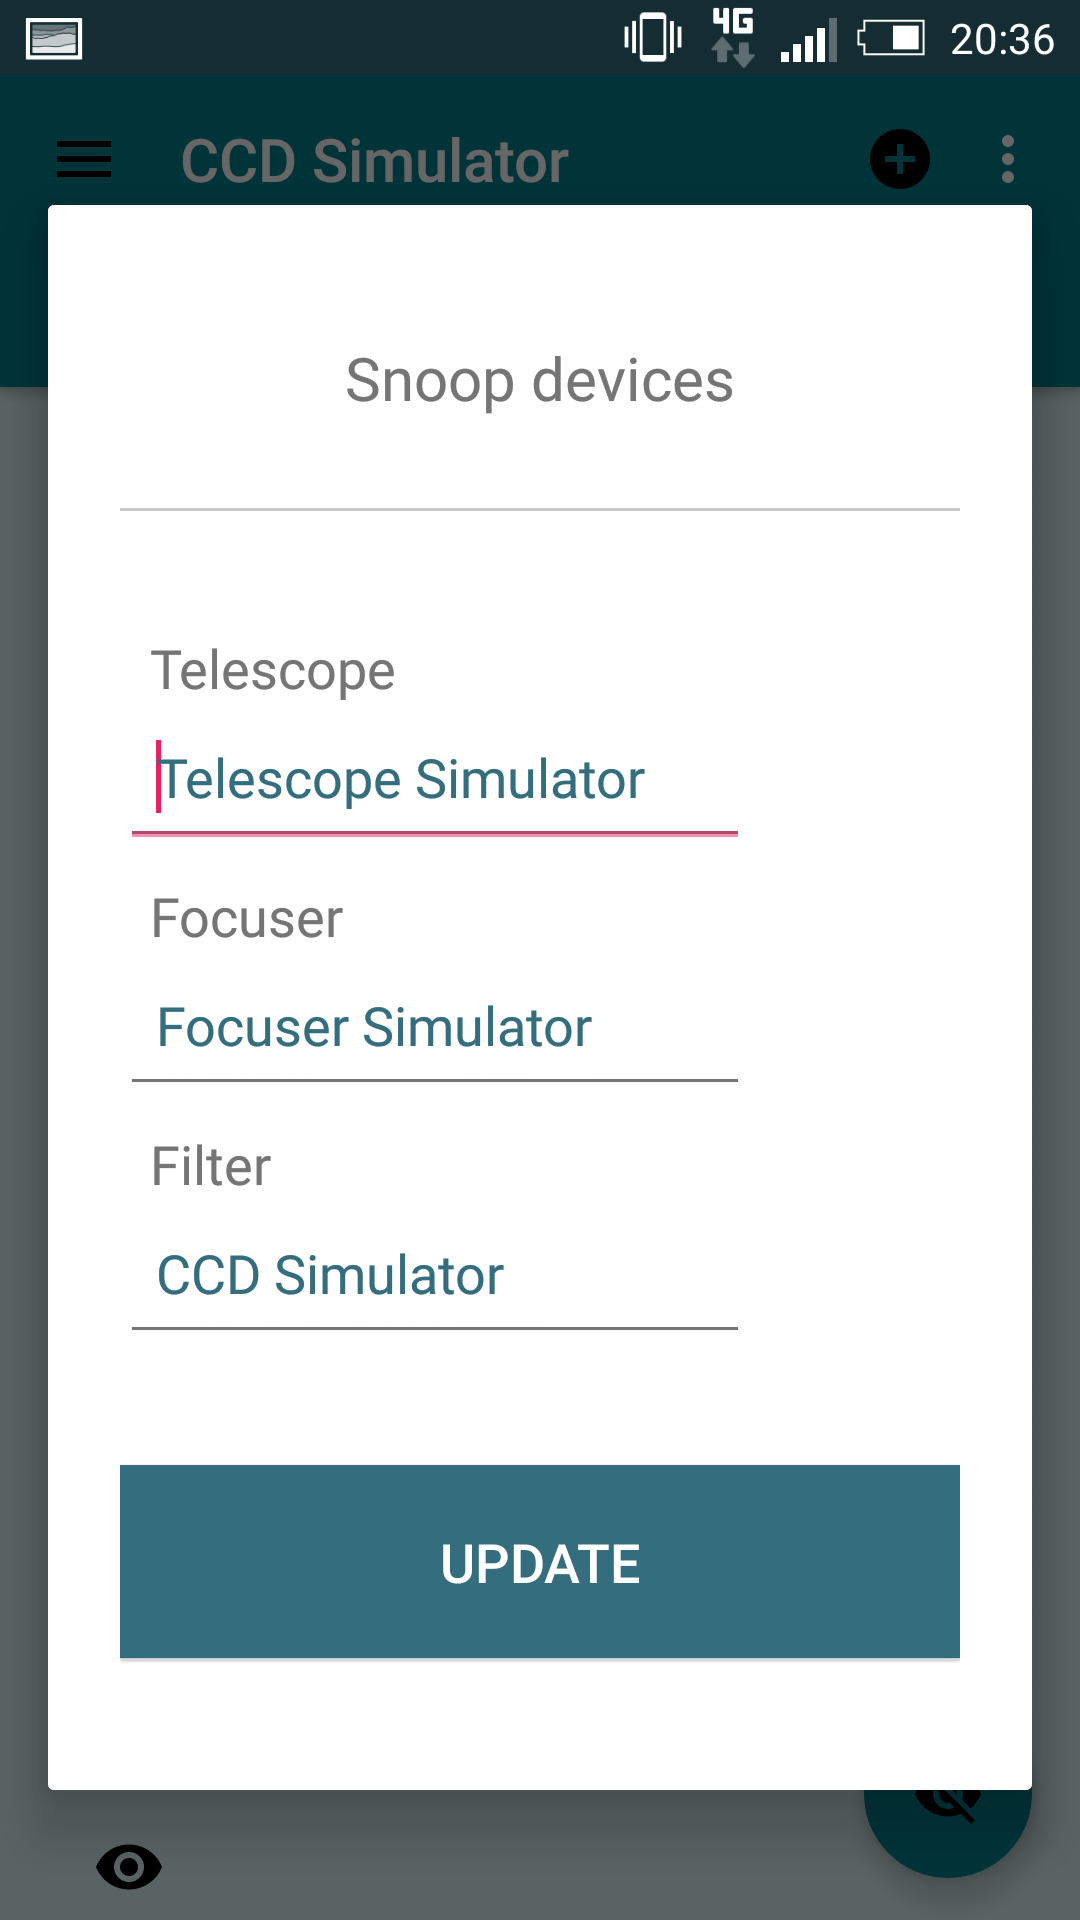
\includegraphics[width=0.3\textwidth]{../images/text_edit_view.png}
  \caption{Dialogo para editar una propiedad text}
  \label{fig:text_edit}
  \end{center}
\end{figure}


\begin{figure}[!ht]
  \begin{center}
  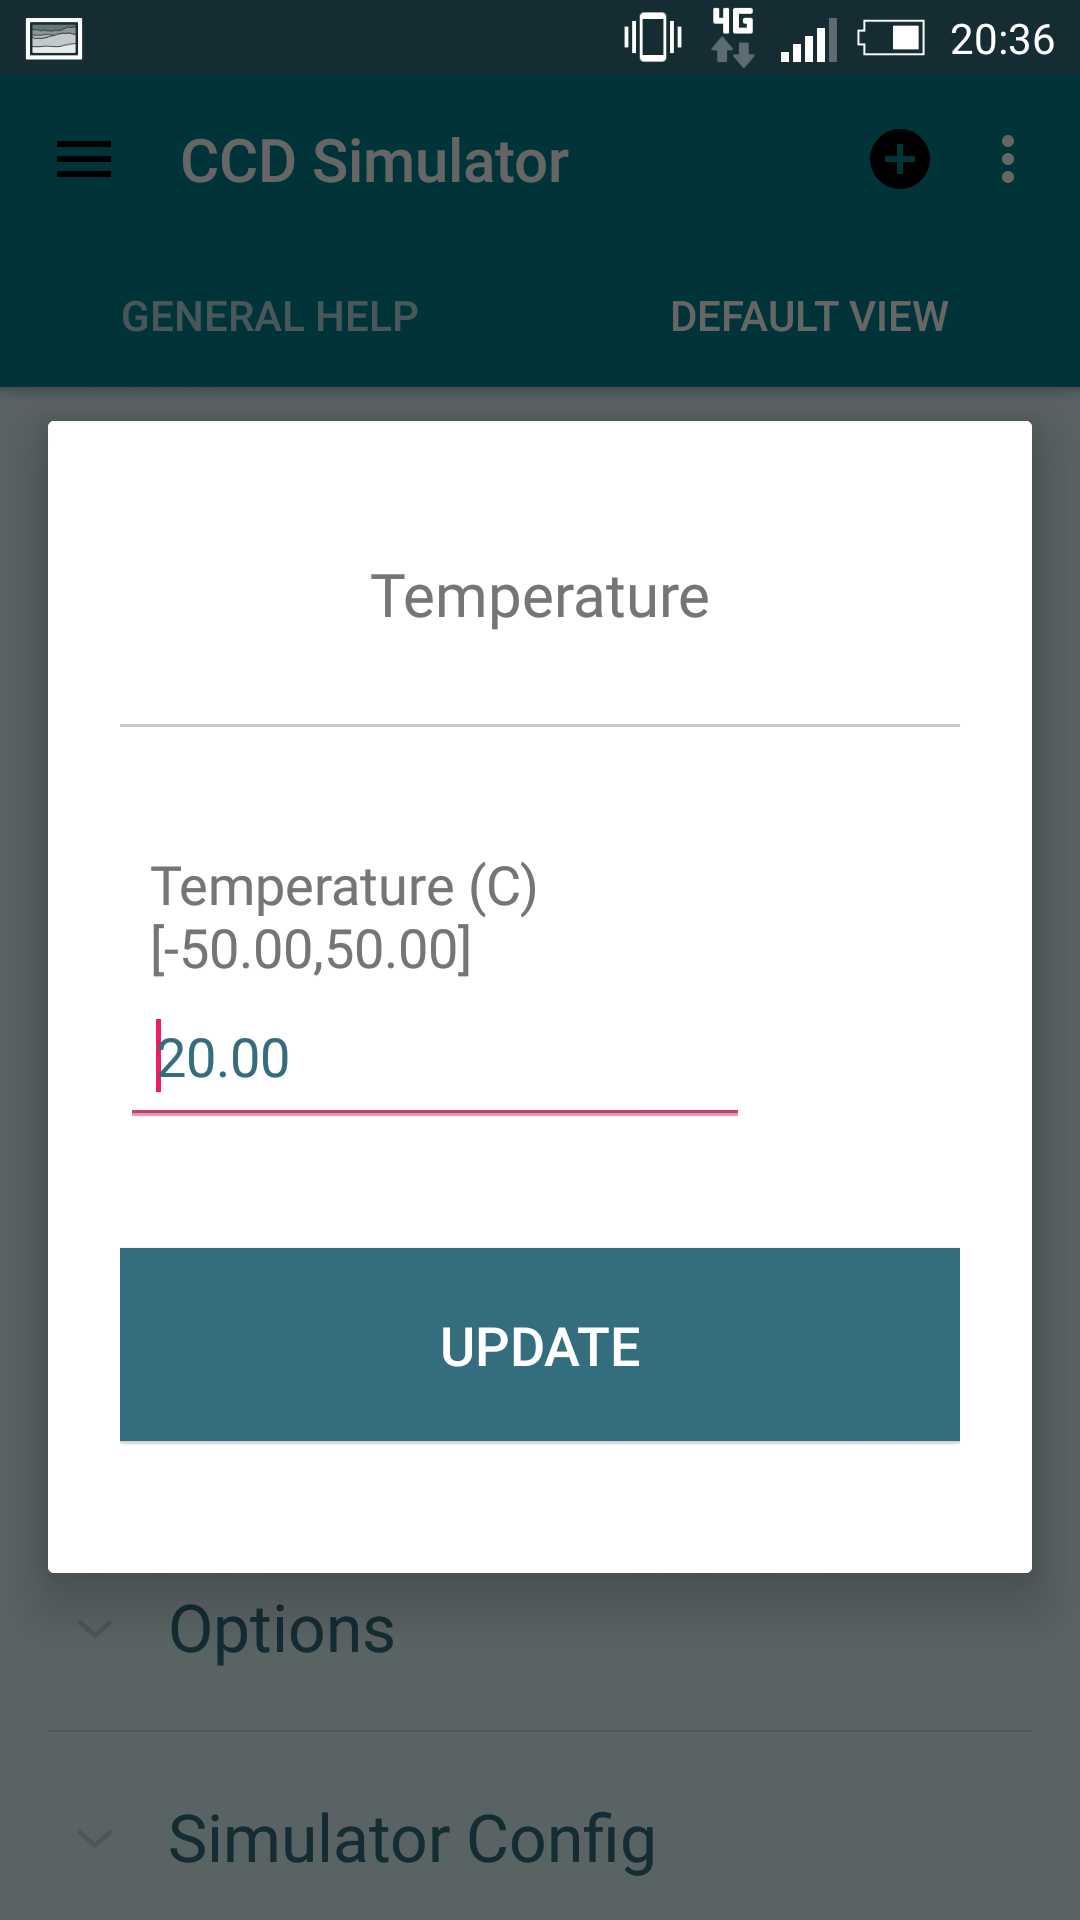
\includegraphics[width=0.3\textwidth]{../images/number_edit_view.png}
  \caption{Dialogo para editar una propiedad number}
  \label{fig:number_edit}
  \end{center}
\end{figure}


\begin{figure}[!ht]
  \begin{center}
  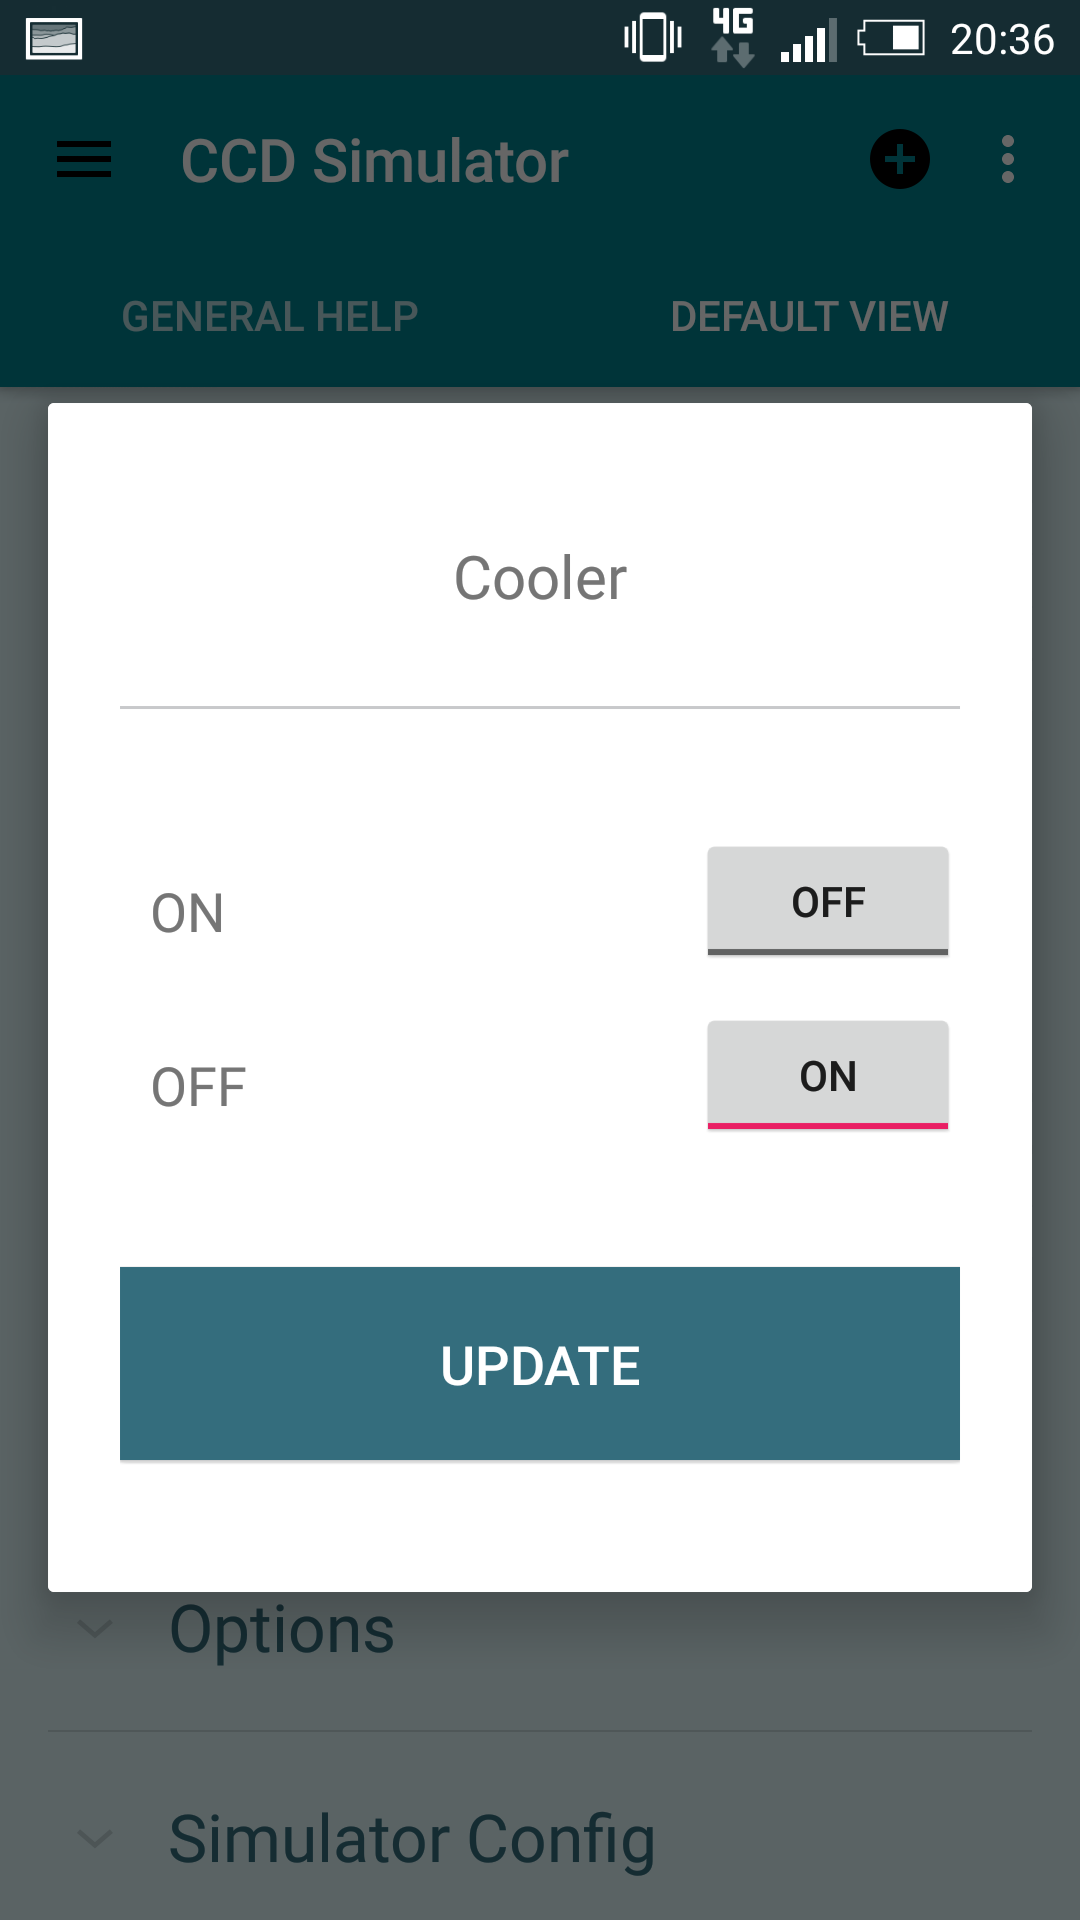
\includegraphics[width=0.3\textwidth]{../images/switch_edit_view.png}
  \caption{Dialogo para editar una propiedad switch}
  \label{fig:number_edit}
  \end{center}
\end{figure}

\bigskip
\subsubsection{Diálogos para gestión de las conexiones}

Estos diálogos permiten añadir, editar o borrar conexiones. Como cada conexión se define por un nombre, un URL del servidor, un puerto y las opciones de activar la recepción de blobs y la autoconexión, todos estos campos son comunes a la vista para añadir y para editar. La vista para editar añade un botón para poder borrar el log de la conexión (figuras \ref{fig:new_connect} y \ref{fig:edit_connect}).


\begin{figure}[!ht]
  \begin{center}
  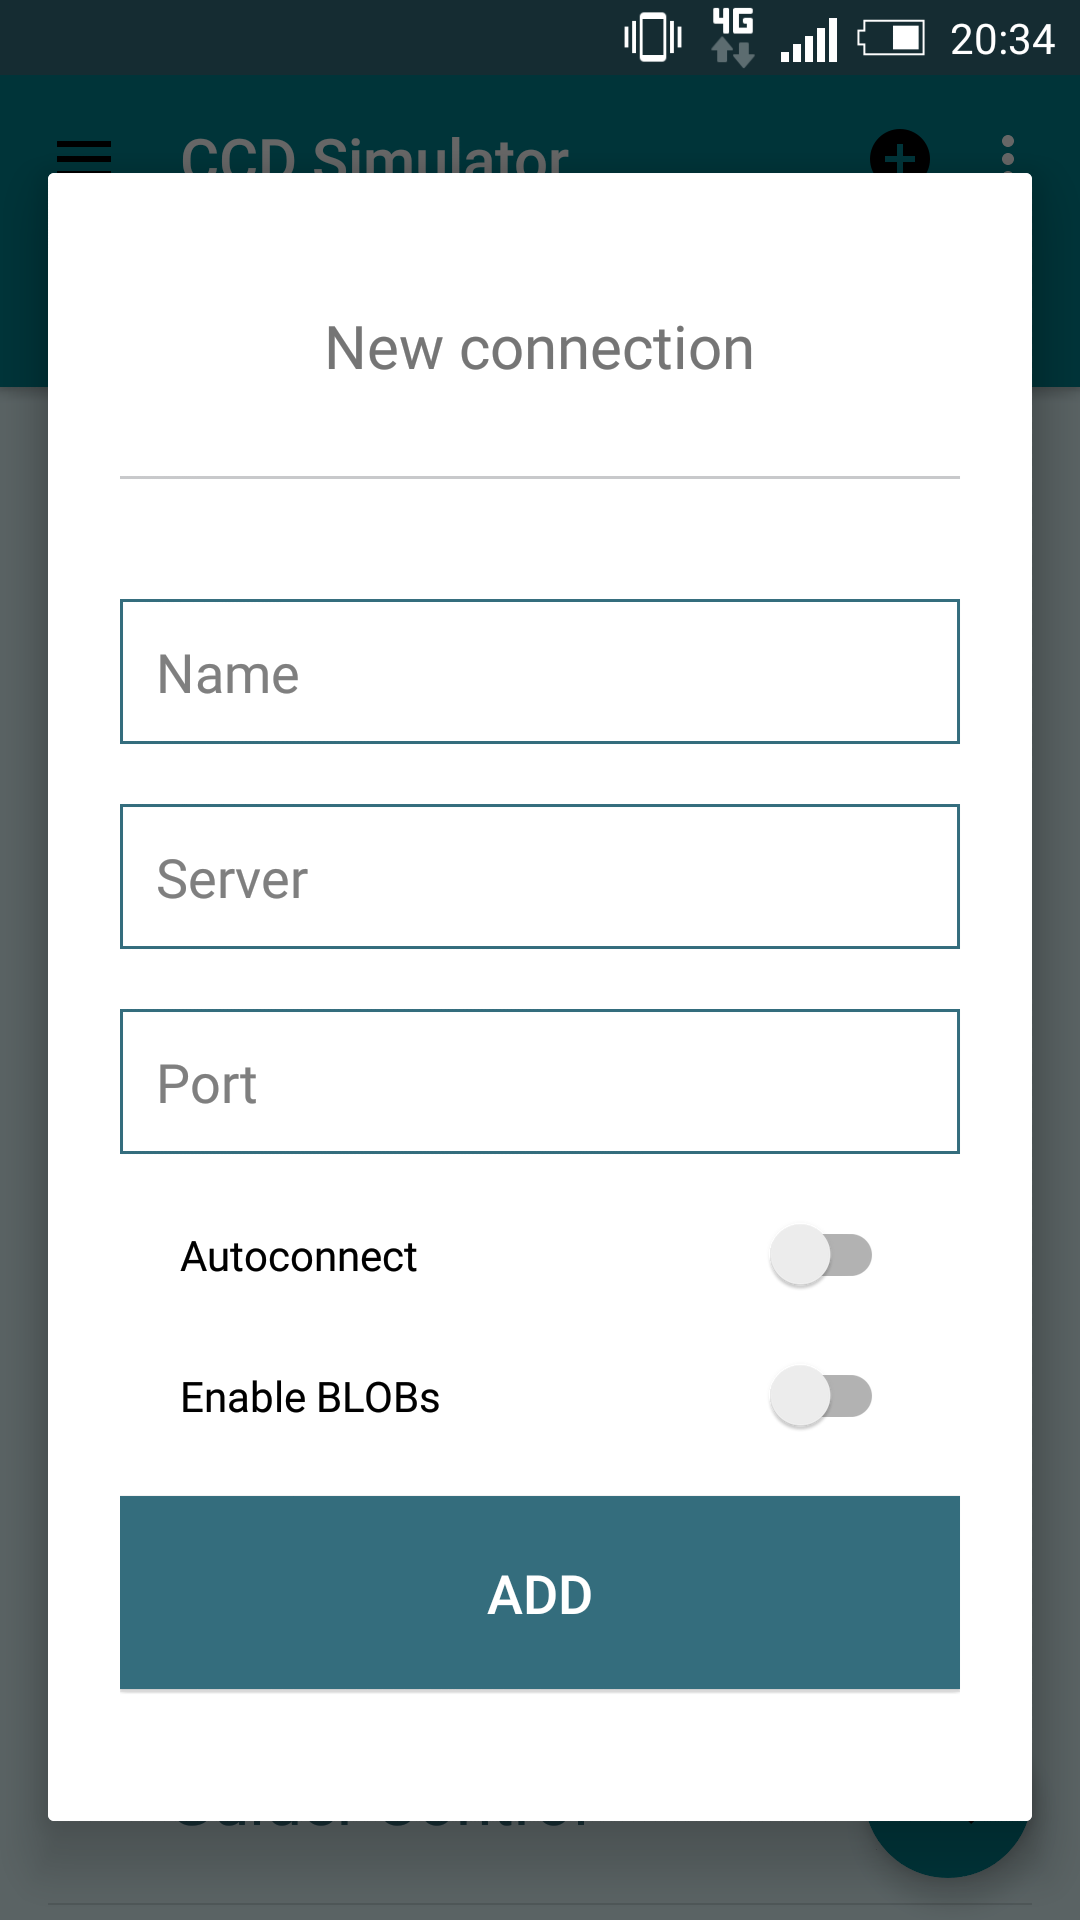
\includegraphics[width=0.3\textwidth]{../images/nueva_conexion.png}
  \caption{Dialogo para añadir una conexión}
  \label{fig:new_connect}
  \end{center}
\end{figure}


\begin{figure}[!ht]
  \begin{center}
  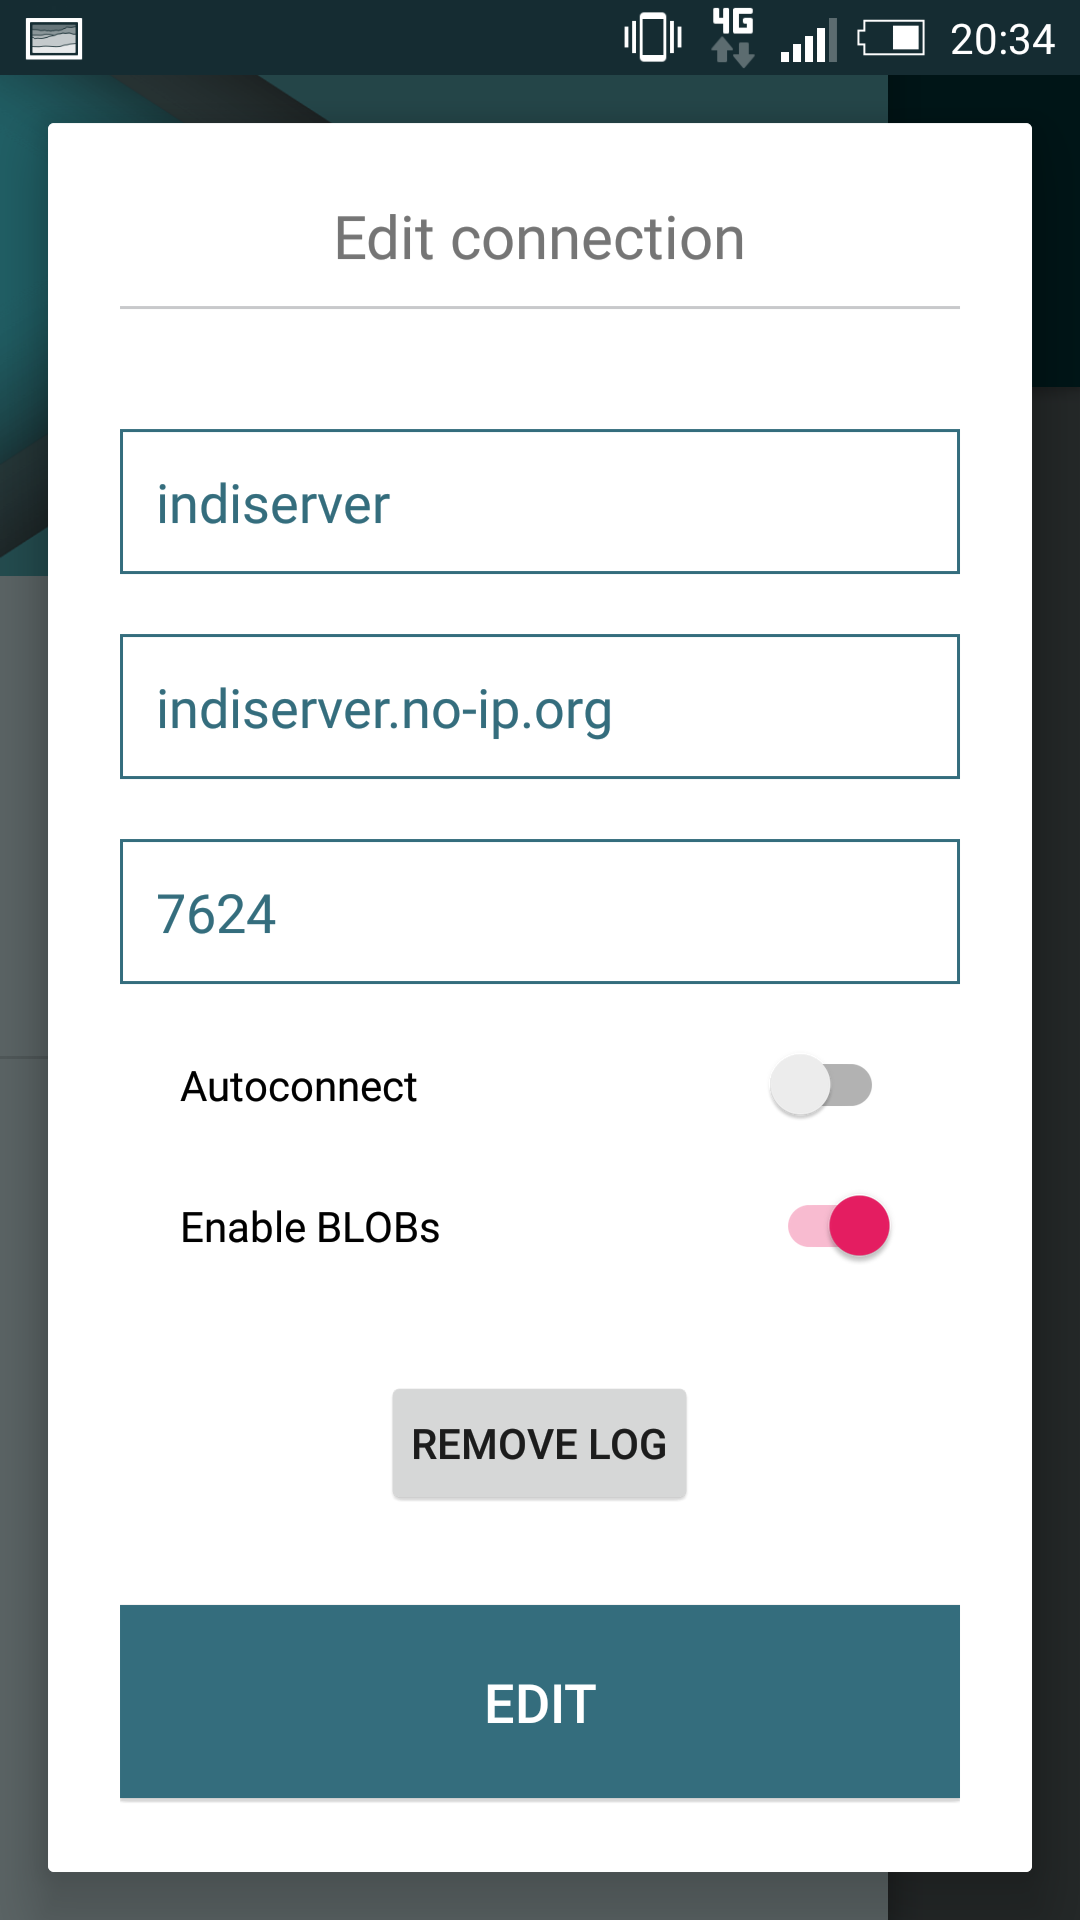
\includegraphics[width=0.3\textwidth]{../images/editar_conexion.png}
  \caption{Dialogo para editar una conexión}
  \label{fig:edit_connect}
  \end{center}
\end{figure}

\bigskip
La vista para borrar conexiones es una simple lista con todas las conexiones que haya y un \textit{checkbox} para marcar las que deseamos borrar (figura \ref{fig:remove_connect}).


\begin{figure}[!ht]
  \begin{center}
  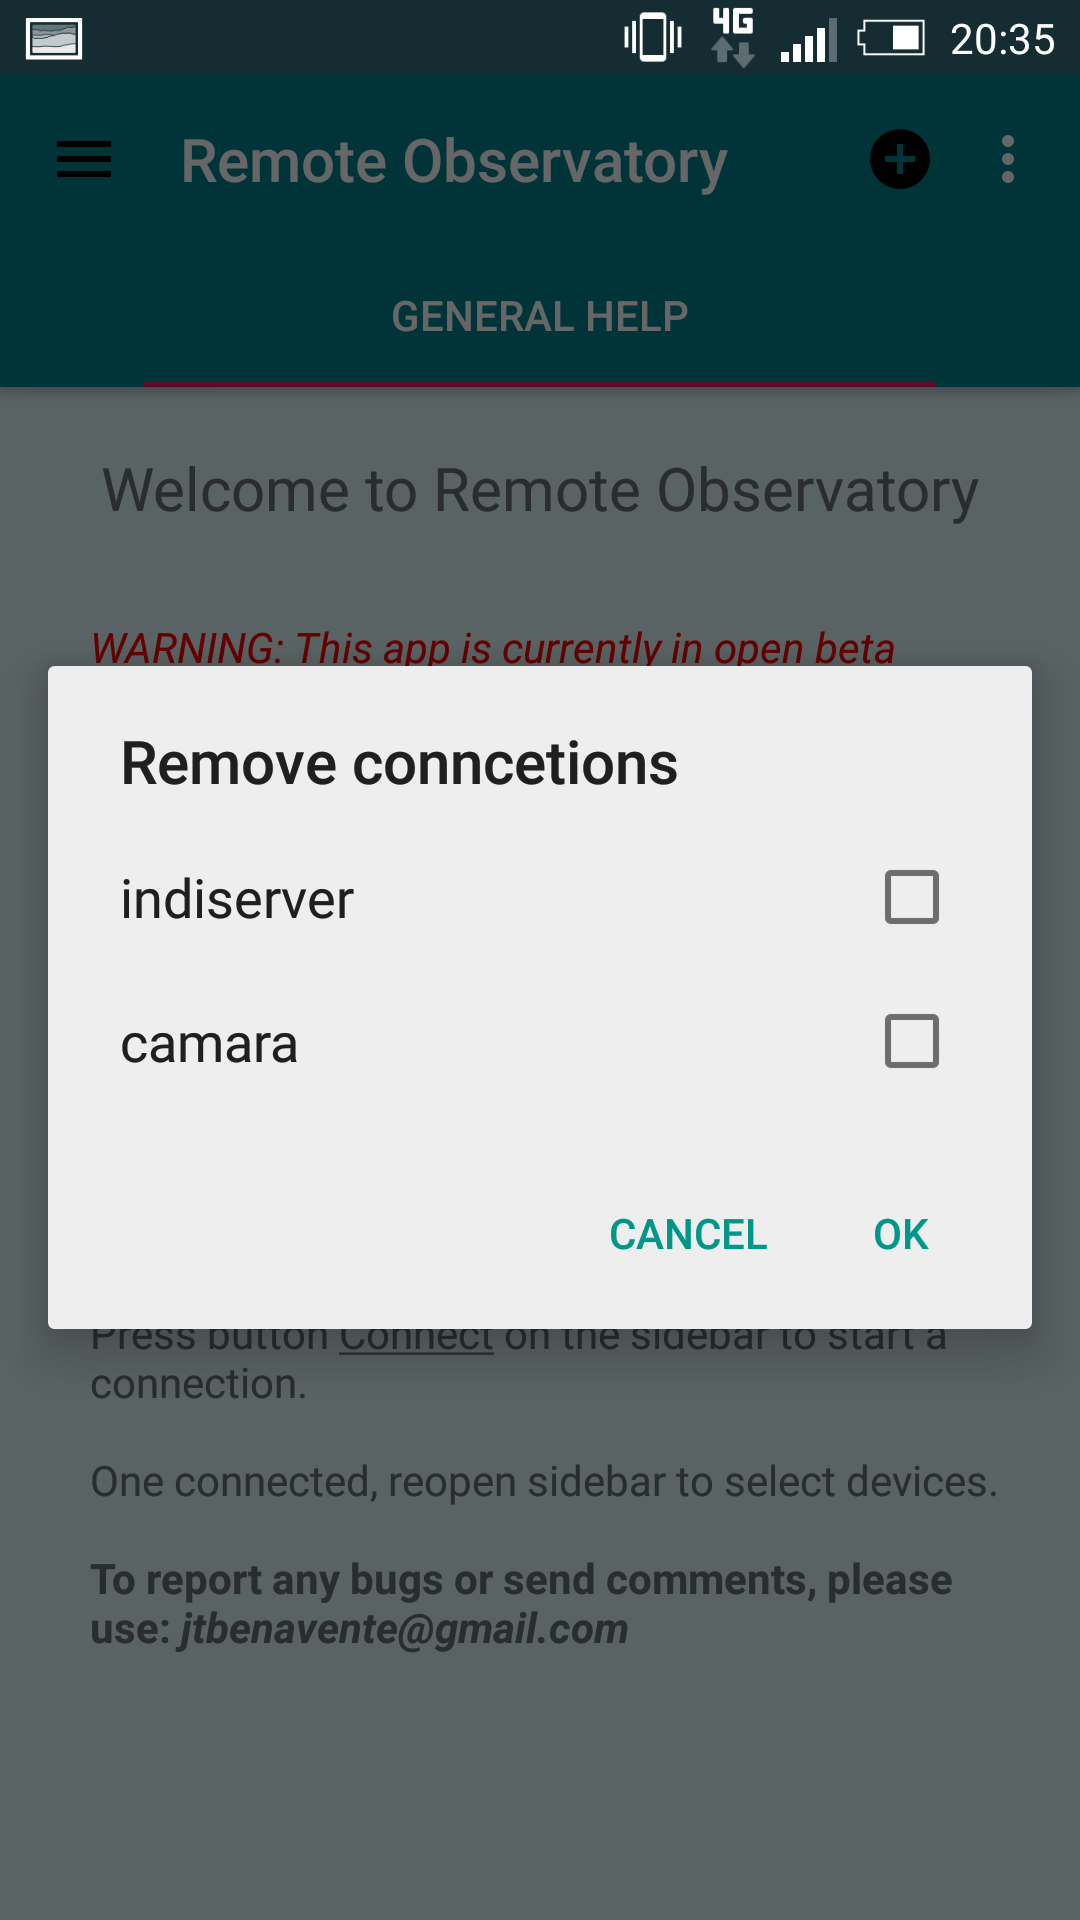
\includegraphics[width=0.3\textwidth]{../images/borrar_conexiones.png}
  \caption{Dialogo para borrar conexiones}
  \label{fig:remove_connect}
  \end{center}
\end{figure}


\bigskip
\subsubsection{Diálogos para informar de errores o avisos}
Estas vistas informan al usuario de un error al introducir datos, errores de desconexión o conexión y de alerta cuando se añaden o quitan nuevos dispositivos (\ref{fig:alert_view}).

\begin{figure}[!ht]
  \begin{center}
  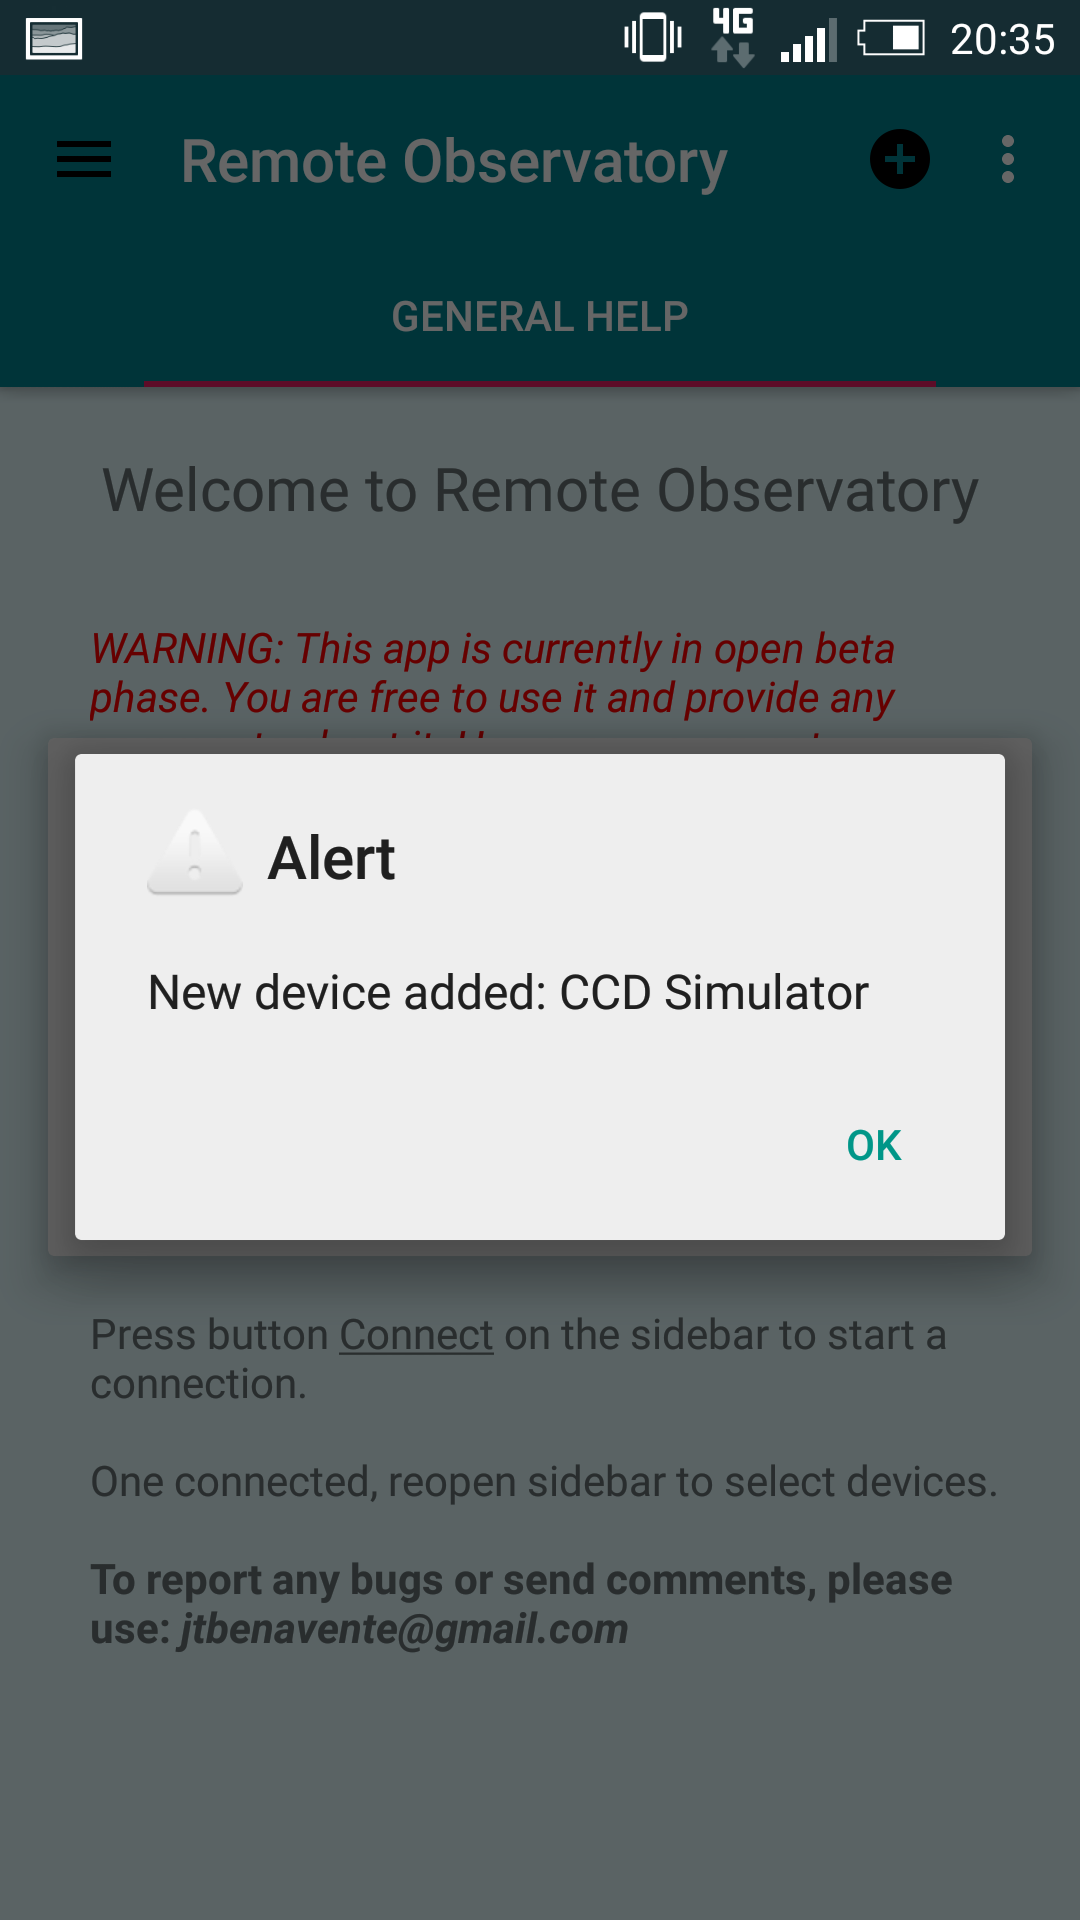
\includegraphics[width=0.3\textwidth]{../images/aviso.png}
  \caption{Dialogo de aviso}
  \label{fig:alert_view}
  \end{center}
\end{figure}


\bigskip
\subsection{Interfaz de log}

Esta es una interfaz muy simple para poder ver los \textit{logs} de cada una de las conexiones guardadas en la aplicación. Para ello se crea una vista tabulada con todas ellas (figura \ref{fig:log_view}).

\begin{figure}[!ht]
  \begin{center}
  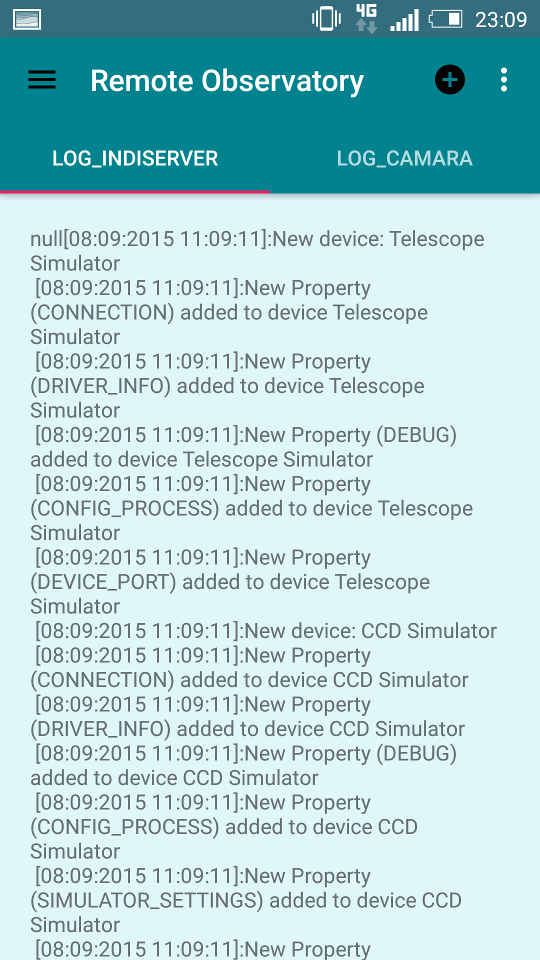
\includegraphics[width=0.3\textwidth]{../images/log2.png}
  \caption{Vista de los ajustes}
  \label{fig:log_view}
  \end{center}
\end{figure}


\bigskip
\subsection{Interfaz de los ajustes}

Los ajustes tienen una vista especial para poder editar las diferentes notificaciones y para poder establecer una carpeta para almacenar los archivos de la aplicación. Como podemos ver en la figura \ref{fig:settings_view}, cada una de las notificaciones tienen un elemento \textit{switch} de \textbf{Android} para marcar el estado. Al final de la vista encontramos un campo editable para poner la ruta que deseemos para la carpeta.


\begin{figure}[!ht]
  \begin{center}
  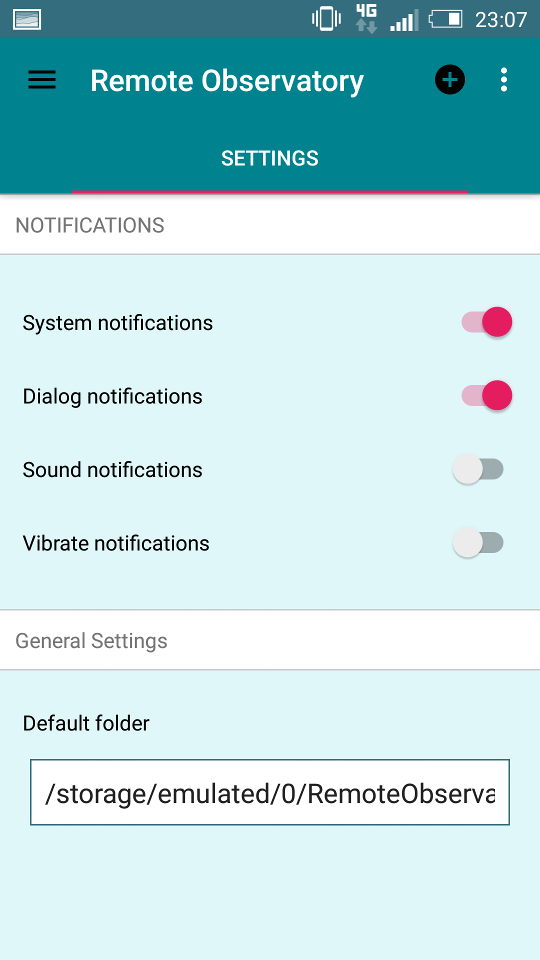
\includegraphics[width=0.3\textwidth]{../images/settings2.png}
  \caption{Vista de los ajustes}
  \label{fig:settings_view}
  \end{center}
\end{figure}


\bigskip
\section{Mecanismo de adición de vistas}

Uno de los objetivos principales del proyecto es facilitar a desarrolladores externos al proyecto, la posibilidad de agregar nuevas clases para gestionar vistas especificas de propiedades y dispositivos, liberando al desarrollador de la necesidad de conocer el código de la aplicación. Para ello se han diseñado una serie de mecanismos y pasos a seguir para poder añadir vistas personalizadas.


\bigskip
\subsection{Propiedades}
Para poder añadir una nueva vista debemos seguir tres pasos:

\begin{itemize}
  \item Crear una clase que implemente la interfaz \textbf{UIPropertyManager}.
  \item Crear una interfaz de usuario para android en XML tanto para la vista de elemento de lista como para la vista para editar una propiedad.
  \item Declarar un objeto de la clase creada y añadirlo al vector de manejadores.
\end{itemize}


\subsubsection{Interfaz UIPropertyManager}

En la sección de diseño de clases hemos podido ver la interfaz que permite crear los distintos tipos de manejadores de propiedades.

\begin{lstlisting}[language=Java,caption={Interfaz UIPropertyManager},label={lst:ui_prop_manager}]

/**
 *  Interface to handle views and indi propertys
 */
public interface UIPropertyManager {
    /**
     *  Check if this class can represent p
     *
     * @param p Indi property
     * @return True/false if class can represent p
     */
    boolean handlesProperty (INDIProperty p);

    /**
     *  Create and return a view sets with p elements
     *
     * @param p Indi property
     * @param inflater Layout inflater to inflate view
     * @param parent ViewGroup to inflate view
     * @param context Context to allow use Activity methods
     * @return View
     */
    View getPropertyView (INDIProperty p, LayoutInflater inflater, ViewGroup parent, Context context);

    /**
     *  update view v with Indi property p elements
     *
     * @param p Indi property
     * @param v View
     */
    void updateView (INDIProperty p, View v);

    /**
     *  Create a new view dialog to allow set Indi property p elements
     *
     * @param p Indi property
     * @param inflater Layout inflater to inflate view
     * @return View
     */
    View getUpdateView(INDIProperty p, LayoutInflater inflater, DialogFragment fragment);

    /**
     *  Update property with change saved at view v
     *
     * @param p Indi property
     * @param v View
     */
    void updateProperty(INDIProperty p, View v);

    /**
     *  Get priority
     *
     * @return priority
     */
    int getPriority();

    /**
     *  Get update button reference
     *
     *  @return update button
     */

    Button getUpdateButton();
}

\end{lstlisting}

\bigskip
Como podemos ver en el fragmento de código \ref{lst:ui_prop_manager}, las funciones que debemos implementar son:

\begin{itemize}
  \item \texttt{handlesProperty}:
  Esta función recibe una propiedad y debe comprobar si puede manejarla o no devolviendo un valor booleano.

  \item \texttt{getPropertyView}:
  Una vez que comprobamos que podemos manejar la propiedad, esta función debe devolvernos la vista ``inflada'' que se mostrará en la lista de propiedades. Los parámetros \tetxit{inflater, parent y context} son necesarios para poder inflar la vista.

  \item \texttt{updateView}:
  Esta función es la que debe coger la vista anteriormente creada, y debe rellenarla a partir de la propiedad p.

  \item \texttt{getUpdateView}:
  Esta función debe crear la vista para el modo de edición de la propiedad. Esta vista se pintará en un diálogo de tipo \texttt{Fragment}. Al igual que antes, necesitamos las variables \tetxit{inflater y fragment} para ``inflar'' la vista.

  \item \texttt{updateProperty}:
  La vista para editar propiedades permite al usuario editar una propiedad. Una vez que el usuario ha terminado la edición, debemos actualizar la propiedad con los valores de la vista y enviar la información al servidor usando la función de la propiedad de \textbf{INDI}, \texttt{sendChangesToDriver}. 

  \item \texttt{getPriority}:
  Esta función debe devolver una valor numérico para establecer la prioridad que tendrá la vista respecto a otras vistas o a la vista por defecto de la propiedad. Cuanto mayor sea el valor, más prioridad tendrá

  \item \texttt{getUpdateButton}:
  Esta función debe devolver un objeto ``Button'' si la vista tendrá el botón para actualizar, o \textit{null} en caso de que no haya botón.
\end{itemize}

\bigskip
Una vez que tenemos la clase creada debemos diseñar la interfaz de usuario en un archivo \textit{XML} como el del archivo del fragmento de código \ref{lst:xml_view} que representa la vista de elemento de lista de la propiedad \textit{Connection}. Además de este, debemos crear otra vista para mostrar en el diálogo de edición de propiedades. No hay ningún tipo de restricción para estas vistas. El desarrollador es libre de poner lo que necesite en ambas interfaces de usuario.

\begin{lstlisting}[language=XML,caption={Vista XML en android},label={lst:xml_view}]
<?xml version="1.0" encoding="utf-8"?>

<RelativeLayout xmlns:android="http://schemas.android.com/apk/res/android"
    android:layout_width="match_parent" android:layout_height="wrap_content"
    android:padding="5dp">

    <ImageView
        android:layout_width="wrap_content"
        android:layout_height="wrap_content"
        android:id="@+id/idle"
        android:layout_marginRight="10dp"
        android:layout_alignParentLeft="true" />

    <TextView
        android:layout_width="wrap_content"
        android:layout_height="wrap_content"
        android:text="New Text"
        android:id="@+id/name"
        android:layout_alignParentTop="true"
        android:layout_toRightOf="@+id/idle"
        android:layout_marginLeft="10dp"
        android:textAppearance="@android:style/TextAppearance.Holo.Large"
        android:textStyle="bold" />
    <TextView
        android:layout_width="wrap_content"
        android:layout_height="wrap_content"
        android:text=""
        android:id="@+id/label"
        android:layout_below="@+id/name"
        android:layout_toRightOf="@+id/idle"
        android:layout_marginTop="10dp"
        android:layout_marginLeft="10dp"
        android:textAppearance="@android:style/TextAppearance.Holo.Medium" />

    <TextView
        android:layout_width="wrap_content"
        android:layout_height="wrap_content"
        android:text=""
        android:id="@+id/type"
        android:layout_below="@+id/label"
        android:layout_toRightOf="@+id/idle"
        android:layout_marginTop="10dp"
        android:layout_marginLeft="10dp"
        android:textAppearance="@android:style/TextAppearance.Holo.Medium" />

    <ImageButton
        android:layout_width="wrap_content"
        android:layout_height="wrap_content"
        android:layout_margin="30dp"
        android:src="@drawable/ic_save_black_24dp"
        android:id="@+id/save_button"
        android:layout_below="@+id/type"
        android:layout_toRightOf="@+id/idle"/>

    <ImageButton
        android:layout_width="wrap_content"
        android:layout_height="wrap_content"
        android:src="@drawable/ic_pageview_black_24dp"
        android:id="@+id/view_button"
        android:layout_alignTop="@+id/save_button"
        android:layout_toRightOf="@+id/save_button"
        android:layout_toEndOf="@+id/save_button" />

    <TextView
        android:layout_width="wrap_content"
        android:layout_height="wrap_content"
        android:id="@+id/perm"
        android:textStyle="bold"
        android:text=""
        android:layout_margin="8dp"
        android:paddingTop="10dp"
        android:paddingLeft="4dp"
        android:layout_alignParentLeft="true"
        android:layout_below="@+id/idle"
        android:textColor="#ff000000" />

    <ImageView
        android:layout_width="wrap_content"
        android:layout_height="wrap_content"
        android:id="@+id/visibility"
        android:layout_margin="10dp"
        android:layout_alignParentLeft="true"
        android:layout_below="@+id/perm"/>

</RelativeLayout>


\end{lstlisting}


\bigskip
Una vez creada la clase y las dos vistas en archivos XML, debemos añadir un objeto de la nueva clase manejadora, a la lista con el resto de objetos para manejar propiedades. Según la prioridad establecida, el nuevo manejador de propiedades se colocarán en una posición concreta. En el segmento de código \ref{lst:property_uis} podemos esta lista. La función que se observa es llamada al inicio del programa para establecer todas las clases que pueden manejar propiedades. Para cada objeto, llamamos al método de la clase \texttt{Config} \texttt{addUiPropertyManager(nuevo manejador)}

\begin{lstlisting}[language=Java,caption={Lista de objetos manejadores de propiedades},label={lst:property_uis}]

private void setUiProperties() {
        //add UI object
        Config.init();
        Config.addUiPropertyManager(new UIBlobPropertyManager());
        Config.addUiPropertyManager(new UITextPropertyManager());
        Config.addUiPropertyManager(new UISwitchPropertyManager());
        Config.addUiPropertyManager(new UINumberPropertyManager());
        Config.addUiPropertyManager(new UILightPropertyManager());
        Config.addUiPropertyManager(new UIConnecPropertyManager());
        Config.addUiPropertyManager(new UIAbortPropertyManager());

    }

\end{lstlisting}

\bigskip
Para ilustrar la posibilidad de añadir nuevas vistas, se han creado dos manejadores nuevos: \textit{connection y abort} (figura \ref{fig:connect_abort}).

\begin{figure}[!ht]
  \begin{center}
  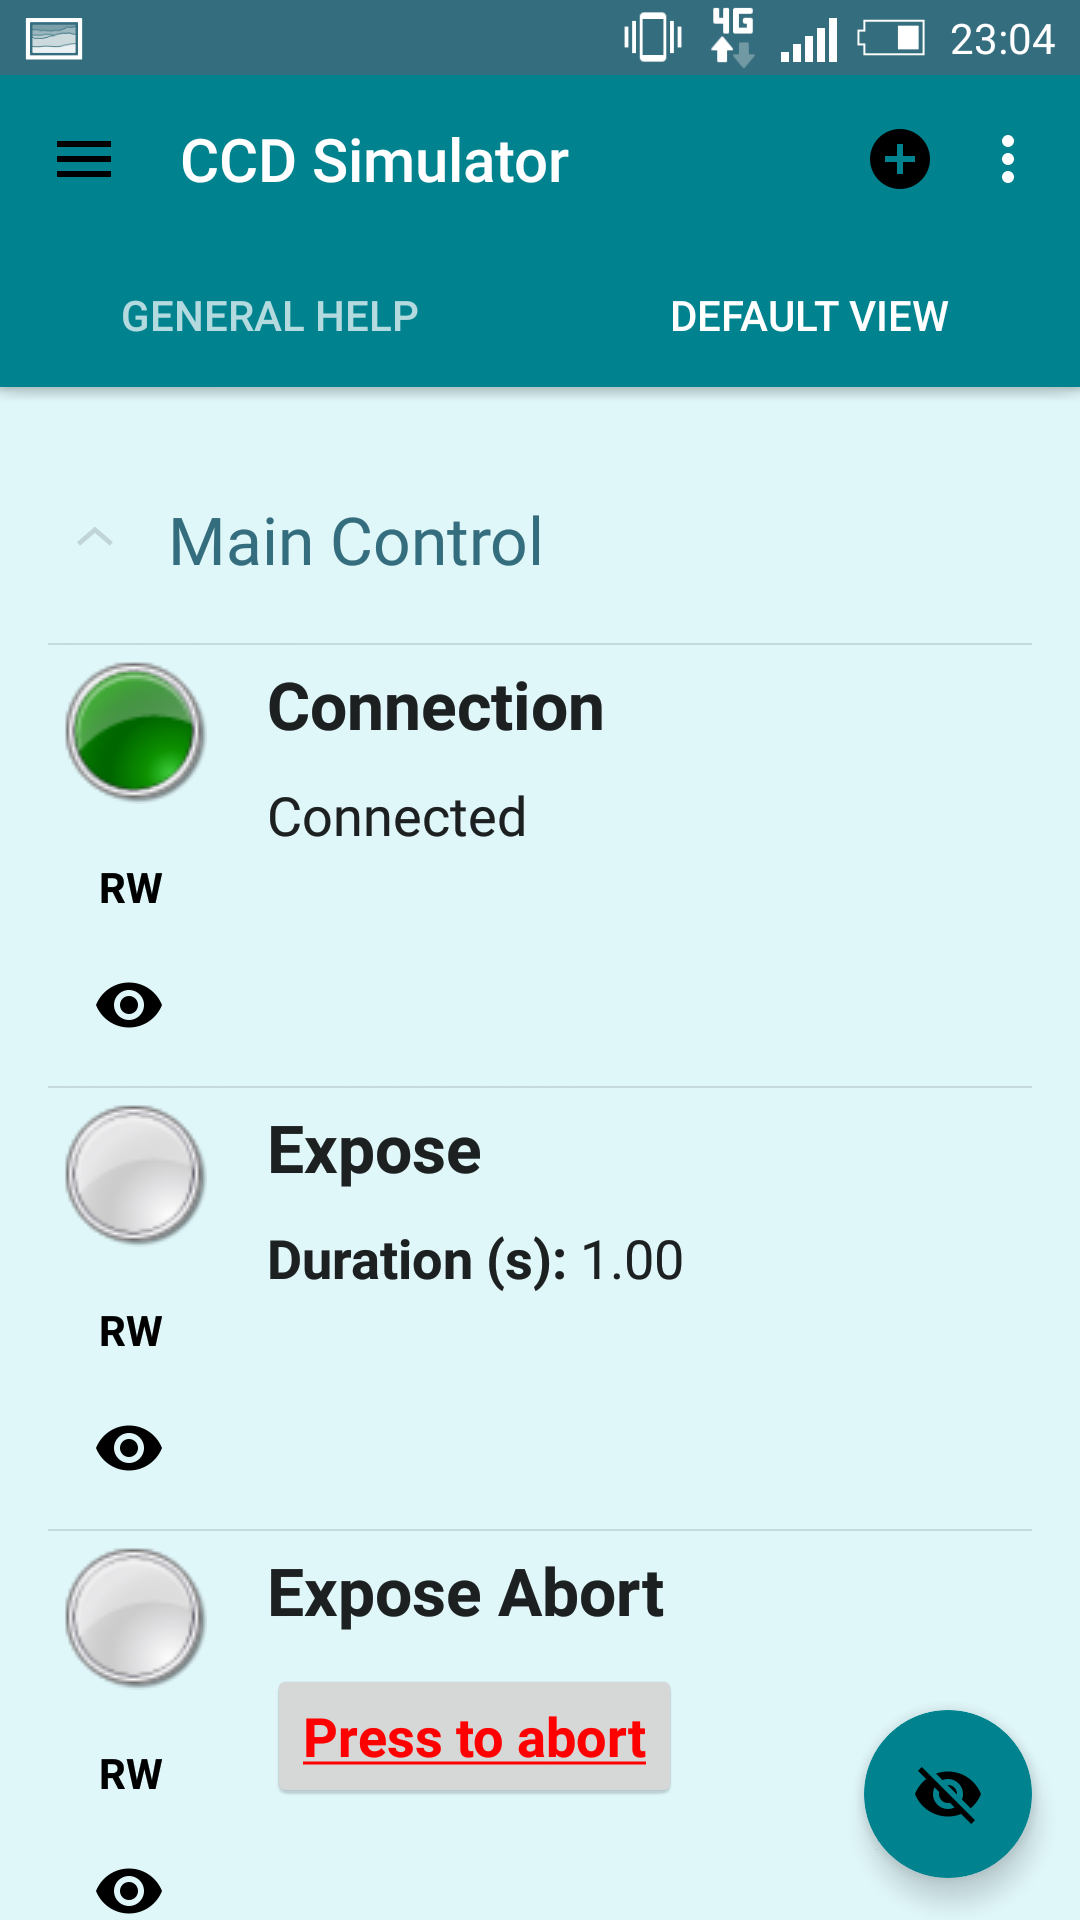
\includegraphics[width=0.3\textwidth]{../images/captura10.png}
  \caption{Vista de las propiedades connection y abort}
  \label{fig:connect_abort}
  \end{center}
\end{figure}

\newpage
\subsection{Dispositivos}
Al igual que con las propiedades, el software está diseñado para facilitar el diseño de nuevas clases para tener vistas especiales para algún dispositivo.

\bigskip
En el caso de las propiedades, se establecían prioridades para poder elegir de entre todas las posibilidades, cual iba a ser la interfaz de la propiedad concreta. En el caso de los dispositivos tenemos una interfaz de usuario por defecto, que lista las propiedades en una lista expandible. Pero se pueden añadir tantas como se deseen, pudiendo pasar de una a otra ya que se irían añadiendo al panel tabulado de la interfaz de usuario principal de la aplicación.

Para poder crear nuevas vistas para un dispositivo se ha diseñado la clase abstracta \texttt{DeviceView}.

\begin{lstlisting}[language=Java,caption={Clase abstracta DeviceView},label={lst:device_view}]
public abstract class DeviceView extends Fragment {

    static Device device;
    protected int layout;

    /**
     *  Check if this class can represent p
     *
     * @param dev Indi property
     * @return True/false if class can represent p
     */
    public abstract boolean handlesDevice (Device dev);

    public abstract String getName();

    @Override
    public abstract View onCreateView(LayoutInflater inflater, ViewGroup container, Bundle savedInstanceState);
}

\end{lstlisting}


\bigskip
Para poder crear una nueva vista de dispositivo debemos:

\begin{itemize}
  \item Crear una clase que herede de \texttt{deviceView}.
  \item Crear un archivo \textit{XML} con la definición de la interfaz de usuario.
  \item Añadir un objeto de la clase a la lista de clases manejadoras de dispositivos.
\end{itemize}


Como podemos ver en el fragmento de código \ref{lst:device_view}, tenemos dos atributos que son el dispositivo que vamos a manejar, y la referencia de \textbf{Android} al recurso donde se encuentra el archivo \textit{XML} con la definición de la vista. Además debemos implementar las siguientes funciones:


\begin{itemize}
  \item \texttt{handlesDevice}:
  Esta función recibe un dispositivo y debe comprobar si puede manejarlo o no devolviendo un valor booleano.

  \item \texttt{getName}:
  Esta función debe devolver el nombre que se desea que aparezca en la parte superior de la vista (vista tabulada).

  \item \texttt{onCreateView}:
  La clase abstracta hereda de \texttt{Fragment} y por ello esta función debe ser implementada, ya que se llamará cuando se llame a la clase para pintar la interfaz de usuario\cite{ALCA}. En ella deberemos crear la vista y realizar todas las inicializaciones que queramos.

\end{itemize}

\bigskip
Al igual que ocurría con las propiedades, debemos crear una vista definiéndola en un archivo \textit{XML} con los elementos visuales de \textbf{Android} que necesitemos.

\bigskip
Por último debemos agregar un objeto de nuestra clase a la lista de manejadores de dispositivos, como se ve en el fragmento de código \ref{lst:device_uis} llamando al método de la clase \texttt{Config} \texttt{addDeviceView(nuevo manejador)}

\begin{lstlisting}[language=Java,caption={Lista de objetos manejadores de dispositivos},label={lst:device_uis}]
private void setDeviceViews() {
    Config.addDeviceView(new DeviceMeteoView());
}

\end{lstlisting}

\bigskip
\section{Implementación}

Para un proyecto de desarrollo de software, las fases de análisis y diseño son claves para realizar la implementación. Uno de los objetivos del un proyecto fin de grado es demostrar la adquisición de competencias para realizar un correcto análisis de requisitos y un diseño exhaustivo. Estas fases previas realizadas correctamente aseguran una implementación más rápida. Por ello, la fase de implementación ha consistido en llevar a cabo todos los diagramas y especificaciones descritas en el diseño.

\bigskip
El código de la aplicación esta publicado bajo una licencia de \textbf{Software Libre} y puede ser consultada en \url{https://github.com/torresj/indi-android-ui}.

\bigskip
Para la implementación de este software, se ha usado el entorno de desarrollo \textbf{Android Studio} (Figura \ref{fig:android_studio}). Este entorno es el recomendado por \textb{Android} para realizar aplicaciones móviles.

\begin{figure}[!ht]
  \begin{center}
    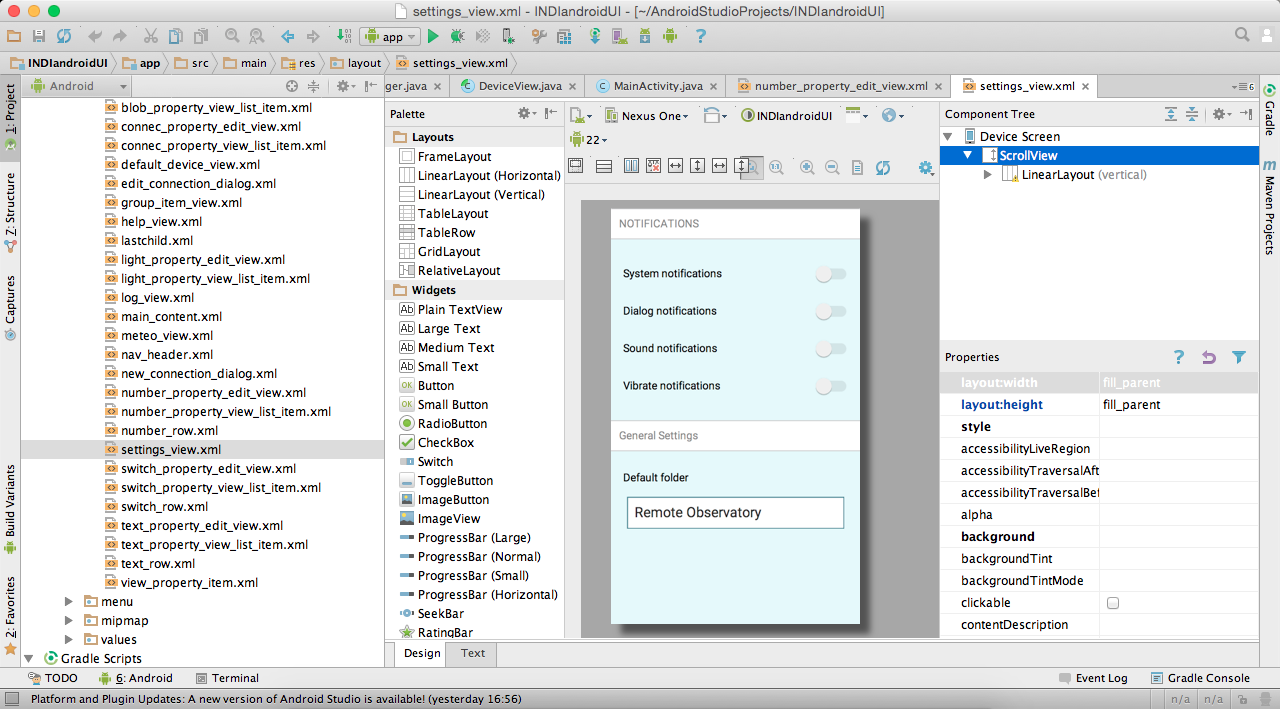
\includegraphics[width=1\textwidth]{../images/android_studio.png}
    \caption{Android Studio}
    \label{fig:android_studio}
  \end{center}
\end{figure}

\bigskip
También se ha usado para el desarrollo el procesador de textos \textbf{Sublime text}.

\bigskip
Para el control de versiones y publicación del código se ha utilizado \textbf{github} y la herramienta en linea \texttt{git} para poder subir los cambios desde un terminal.
\chapter{Pruebas}

Una vez diseñada la aplicación y realizada la implementación, debemos asegurarnos de que todas las partes funcionan y cumplen los objetivos. Para ellos debemos iniciar la fase de pruebas, si bien es cierto que algunas pruebas se han realizada durante el proceso de implementación. Además, al utilizar una metodología de desarrollo basada en iteraciones, debemos tener en cuenta que cada una de las iteraciones ha tenido una fase final, previa a la entrega, de pruebas.

\bigskip
Podemos agrupar las pruebas de la aplicación en:

\begin{itemize}
  \item \textbf{Pruebas unitarias.}
  \item \textbf{Pruebas de integración.}
  \item \textbf{Pruebas de sistema.}
  \item \textbf{Pruebas de aceptación.}
\end{itemize}


\bigskip
\section{Pruebas Unitarias}

Las pruebas unitarias son test realizados por el equipo de desarrollo y que que se deben llevar a cabo subdividiendo las aplicaciones al nivel de clases o módulos faciles de probar e independientes unos de otros. Estos test requieren cambiar el código para ser realizados, comprobando que cada modulo realiza la función esperada, que maneja los rangos de datos de entrada, su comportamiento al forzar los errores, etc.

Para las pruebas unitarias se ha dividido la aplicación en los siguientes módulos:

\begin{itemize}
  \item \textbf{Conexión INDI.}
  \item \textbf{Lista de propiedades}
  \item \textbf{Manejadores de pròpiedades}
  \item \textbf{Creación de ficheros de configuración}
\end{itemize}


\subsection{Conexión INDI}

La conexión con un servidor INDI es vital para el desarrollo del resto de la aplicación. Por ello, en la primera iteración del proceso \textbf{Scrum} se marcó como requisito realizar una clase para implementar un cliente INDI. El objetivo era testear que podíamos conectarnos y obtener dispositivos y propiedades.

\bigskip
Para la consecución de la prueba se ha montado un servidor en una \textit{raspberry Pi} con varios simuladores INDI.

\subsubsection{Objetivo de la prueba}

El objetivo de la prueba es comprobar la correcta conexión a un servidor \textbf{INDI} desde una aplicación \textbf{Android} utilizando las bilbiotecas de \textbf{INDI for Java}.

\subsubsection{Descripción de la prueba}

Se van a comprobar todos los posibles caminos de ejecución para asegurar que el módulo funciona correctamente:

\begin{itemize}
  \item \textbf{Conexión a un servidor:} Nos conectamos a un servidor para comprobar el exito del proceso.
  \item \textbf{Desconexión de un servidor:} No desconectamos de un servidor para comprobar el éxito del proceso.
  \item \textbf{Nos conectamos y apagamos el servidor:} Probamos la gestión de errores al caerse el servidor.
  \item \textbf{Conexión a un servidor con datos erróneos:} Comprobamos la conexión cuando los datos son erróneos o el servidor está desconectado o inaccesible.
\end{itemize}

\subsubsection{Criterio de completitud}

Las pruebas serán satisfactorias si el módulo gestiona correctamente todos los casos definidos anteriormente, y además se conecta de forma satisfactoria al servidor.

\bigskip
\subsection{Listas de propiedades}

Comprobamos que la clase que debe mostrar elementos funciona correctamente. Este módulo recibe como entrada un conjunto de propiedades y devuelve una lista para ser mostrada por pantalla.

\subsubsection{Objetivo de la prueba}

El objetivo de la prueba es comprobar que maneja correctamente un conjunto de datos de entrada para crear las listas de propiedades agrupadas por grupos

\subsubsection{Descripción de la prueba}

La prueba consiste en crear una lista de entrada con propiedades y comprobar que la salida es una lista de dos niveles con las propiedades agrupadas según su grupo. Para ellos e han realizado las siguientes comprobaciones:

\begin{itemize}
  \item \textbf{Lista con distintos tipos de propiedades:} Creamos una lista de propiedades de distintos grupos y comprobamos la construcción de la lsita de dos niveles.
  \item \textbf{Añadir una propiedad de un grupo nuevo:} Se añade una propiedad nueva perteneciente a un grupo aún sin crear.
  \item \textbf{Añadir una propiedad nueva con grupo ya existente:} Se añade una propiedad con un grupo que ya tiene más elementos.
  \item \textbf{Borramos una propiedad perteneciente a un grupo con más elementos:} Borramos una propiedad y comprobamos que se borra del grupo concreto.
  \item \textbf{Borramos una propiedad perteneciente a un grupo cuyo único elemento es la propia propiedad:} Borramos una propiedad de un grupo que quedará vacío al borrarla, por loq ue debe desaparecer.   
\end{itemize}

\subsubsection{Criterio de completitud}

Las pruebas serán satisfactorias si el módulo gestiona correctamente todos los casos definidos anteriormente, creando y borrando convenientemente las propiedades y grupos


\bigskip
\subsection{Manejadores de propiedades}

Los manejadores de propiedades deben, además de crear interfaces de usuario, gestionar la edición de cada una de las propiedades, manejando los errores deribados de entradas de datos erróneos.

\subsubsection{Objetivo de la prueba}

El objetivo de la prueba es comprobar que las clases de cada una de las propiedades, son capaces de procesar los datos de entrada y gestionar los errores deribados de ellos.

\subsubsection{Descripción de la prueba}

La prueba consiste en realizar una batería de test de entrada para cada una de las propiedades comprobando:

\begin{itemize}
  \item \textbf{Datos fuera de rango (propiedad number).}
  \item \textbf{Datos en formato erróneo (propiedad number)}
  \item \textbf{Datos que no cumplan las condiciones de la propiedad (reglas en las propiedades Switch)}  
\end{itemize}

\subsubsection{Criterio de completitud}

Las pruebas serán satisfactorias si el módulo gestiona correctamente todos los casos definidos anteriormente, informando de las distintos errores y gestionandolos correctamente.

\bigskip
\subsection{Creación de ficheros de configuración}

La aplicación debe ser capaz de crear una serie de ficheros de configuración para guardar información de forma permanente.

\subsubsection{Objetivo de la prueba}

Comprobar la creación correcta de los ficheros si no existen, o añadir los datos necesarios en caso de que ya existan

\subsubsection{Descripción de la prueba}

La prueba consiste iniciar el proceso de creación de ficheros de configuración, teniendo en cuento los casos en que los ficheros existan o que no existan.

Hay que tener en cuenta que si existen, se debe añadir la información al final del archivo o sustituir el contenido según el caso.


\subsubsection{Criterio de completitud}

Las pruebas serán satisfactorias si el módulo gestiona correctamente todos los casos definidos anteriormente, creando y/o editando correctamente los ficheros de configuración.

\newpage
\section{Pruebas de integración}

Las pruebas de integración nos permiten comprobar que las combinaciones entre modulos funcionan correctamente. Es habitual comprobar en este tipo de pruebas que los módulos de más bajo nivel se comunican correctamente con las interfaces de usuario verificando que las especificaciones de diseño sean alcanzadas.

Para este proyecto se han realizado las siguientes pruebas:

\begin{itemize}
  \item \textbf{Conexión y desconexión con un servidor.}
  \item \textbf{Interacción con las propiedades.}
  \item \textbf{Gestión de las conexiones.}
  \item \textbf{Ajustes generales.}
\end{itemize}



\subsection{Conexión con un servidor}

En las pruebas unitarias hemos podido comprobar el módulo que realiza la conexión con el servidor. Ahora vamos a comprobar su integración en el resto de la aplicación.


\subsubsection{Objetivo de la prueba}

El objetivo es comprobar cómo el módulo de conexión con el servidor se integra con el resto de clases de la interfaz para mostrar los dispositivos y actualizar cualquier cambio en tiempo real que pueda sufrir cualquier dispositivo o propiedad

\subsubsection{Descripción de la prueba}

Para poder comprobar que la interacción entre el módulo que gestiona la conexión con el servidor y el resto de clases de la interfaz funciona correctamente, debemos realizar las siguientes comprobaciones:

\begin{itemize}
  \item \textbf{Conexión y desconexión con un simulador.}
  \item \textbf{Conexión y desconexión con equipos reales.}
\end{itemize}

Montamos un servidor de pruebas con varios dispositivos simulados y realizamos conexiones y desconexiones comprobando que el servidor está encendido y apagado. Además, teniendo una conxión abierta, apagamos el servidor y/o desconectamos algún dispositivo para ver como el sistema gestiona la situación.

\bigskip
Por último realizamos las mismas comprobaciones pero utilizando un telescopio y una camará.

\subsubsection{Criterio de completitud}

Las pruebas serán satisfactorias siempre y cuando el sistema nunca falle, gestionando cualquier situación de error y permitiendo la conexión y desconexión de servidores simultáneamente, mostrando los dispositivos y las propiedades.


\subsection{Interacción con las propiedades}

Una de las pruebas unitarias consistía en comprobar las clases que gestionan las propiedades. El siguiente paso es comproba su integración con las distintas vistas para editaras, su correcta comunicación y la gestión de los datos de entrada.


\subsubsection{Objetivo de la prueba}

El objetivo es comprobar que podemos cambiar las propiedades a partir de unos datos introducidos en las vistas de la interfaz de usuario.

\subsubsection{Descripción de la prueba}

Para cada propiedad, selecionaremos la vista de edición, y cambiaremos los paremtros utilizando: datos correctos, dato mal construidos y datos fuera de rango. El sistema debe gestionar los errores para cada una de las propiedades:


\begin{itemize}
  \item \textbf{Text.:} Editaremos una propeidad text y comprobaremos que se realiza el cambio correctamente.
  \item \textbf{Number:} Editaremos los elementos de una propiedad \textit{number} con valores correctos, con formato erróneo y fuera de rango.
  \item \textbf{Switch:} Editaremos los elementos de una propiedad \textit{switch} con valores correctos y forzando situaciones que contravengan las reglas de la propiedad, como tener varias opciones activadas cuando solo se permite una, o desactivar todas las opciones cuando tiene que haber al menos una activa.
\end{itemize}


\subsubsection{Criterio de completitud}

Las pruebas serán satisfactorias siempre y cuando el sistema nunca falle, gestionando cualquier situación de error y permitiendo editar la propiedad o informando de cualquier problema con los datos.

\subsection{Gestión de las conexiones}

Una de las configuraciones más importantes que se guardan en memoria son las conexiones, para tenerlas memorizadas aunque cerremos la aplicación. Para esta prueba debemos comprobar que el módulo de configuraciones guarda, borra, edita y crea correctamente las conexiones según las acciones llevadas a cabo por el usuario en la interfaz.


\subsubsection{Objetivo de la prueba}

El objetivo es comprobar que podemos crear,borrar y editar conexiones, y que estos cambios son guardados por la aplicación.

\subsubsection{Descripción de la prueba}

Para poder comprobar la gestión de las conexiónes, primero realizamos las siguientes comprobaciones básicas:


\begin{itemize}
  \item \textbf{Creamos una conexión.}
  \item \textbf{Editamos una conexión.}
  \item \textbf{Borramos una conexión.}
\end{itemize}

\bigskip
Además de realizar estas acciones, comprobaremos que al cerrar la aplicación y al abrirla se mantiene la integridad de los datos.

\subsubsection{Criterio de completitud}

Las pruebas serán satisfactorias siempre y cuando el sistema nunca falle, almacenando correctamente las conexiones y mostrándolas para su interacción con el usuario.

\subsection{Ajustes generales}

La aplicación cuenta con unas sencillas opciones de configuración para activar o desactivar los distintos tipos de notificaciones y la ruta de la carpeta por defecto en el sistema. Debemos comprobar que la activación de cada una de ellas provoca la consiguiente acción cuando se reciben notificaciones.


\subsubsection{Objetivo de la prueba}

El objetivo es doble. Por un lado, poder cambiar el estado de las opciones y que están sean persistentes aunque cerremos la aplicación.

\bigskip
Por otro lado se debe comprobar que la activación de cada una de ellas permite la notificación concreta al recibir cualquier cambios en los dispositivos o en las conexiones.


\subsubsection{Descripción de la prueba}

Las opciones de configuración de las notificaciones son:

\begin{itemize}
  \item \textbf{Notificaciones del sistema:} Activa la recepción de avisos cuando la aplicación está en segundo plano.
  \item \textbf{Notificaciones mediante dialogos emergentes:} Activa las notificaciones mediante un dialogo informando del acontecimiento ocurrido.
  \item \textbf{Notificaciones por sonido:} Activa la reproducción de un sonido al recibir una notificación.
  \item \textbf{Notificaciones por vibración:} Activa la vibración del dispositivo móvil al recibir una notificación.
\end{itemize}

\bigskip
La prueba consiste en activar cada una de ellas y conectarnos a un servidor de pruebas. Cada vez que se pierde la conexión con un servidor se envía una notificación por lo que aprovechamos esta situación para probar cada una de las distintas notificaciones. Ademas estas pruebas las realizamos utilizando dispositivos emulados y dispositivos reales.

\bigskip
Por último, comprobamos que el estado de las opciones es permanente aunque cerremos la aplicación, es decir, cada vez que modificamos cualquier opción, esta queda guardada en la configuración.

\subsubsection{Criterio de completitud}

Las pruebas serán satisfactorias siempre y cuando el sistema nunca falle al recibir una notificación, y que para cada una de las opciones de configuración, se produzca la acción adecuada.


\newpage
\section{Pruebas de sistema}

\chapter{Difusión del proyecto}

Dada la practicidad del proyecto y que existe realmente una demanda del mismo (limitada pero existente) se han llevado a cabo diversas actividades para conseguir la máxima difusión del mismo:

\begin{itemize}
  \item Página Web del proyecto.
  
  \item Publicación en la Google Play.
  
  \item Mantenimiento del repositorio en GitHub.
  
  \item Difusión en la página oficial de la biblioteca INDI.
  
  \item Difusión en el foro oficial de la biblioteca INDI.
\end{itemize}

En las siguientes secciones se comentan más en detalle cada una de dichas actividades.

\section{Página web del proyecto}

\begin{figure}
 \centering
 \includegraphics[width=12cm]{../images/webpage2.jpg}
 % webpage.jpg: 0x0 pixel, 300dpi, 0.00x0.00 cm, bb=
 \caption{Captura de la Página Web en Firefox (PC, Linux)}
 \label{fig:web}
\end{figure}

Se ha registrado el siguiente dominio: \url{http://remoteobservatory.info} así como contratado un hosting para poder crear una página web del proyecto (figura \ref{fig:web}). La idea principal de dicha página es dar a conocer la aplicación de un modo visual y atractivo. Aunque probablemente el público objetivo de la misma no necesite grandes alicientes visuales para decidir probarla, se e ha querido dar un diseño actual. Se han tenido en cuenta las siguientes consideraciones a la hora de crear dicho sitio web:

\begin{itemize}
  \item Crear un sitio claro, directo y con la información más relevante sobre la aplicación: descripción del proyecto, ayuda (incluyendo el manual de usuario) y una sección de descargas.
  
  \item Crear un sitio visualmente atractivo y \textit{responsive} para asegurarnos que se ve de manera adecuada tanto en ordenadores personales como en dispositivos móviles (figura \ref{fig:webMovil}).
  
  \item Ilustrar el sitio con algunas imágenes que intenten transmitir la idea fundamental del proyecto: poder controlar dispositivos astronómicos de manera sencilla desde un móvil.
  
  \item Ofrecer claramente información de contacto con el desarrollador de la aplicación para que sea fácil establecer canales de comunicación entre los usuarios y el mismo (indispensable para depurar errores y obtener ideas sobre posibles nuevas funcionalidades).
  
  \item Dotar a la página de ciertos toques de humor geek que probablemente saquen alguna sonrisa a los aficionados a la astronomía.
\end{itemize}


\begin{figure}
 \centering
 \includegraphics[width=6cm]{../images/webMovil.jpg}
 % webpage.jpg: 0x0 pixel, 300dpi, 0.00x0.00 cm, bb=
 \caption{Captura de la Página Web en Teléfono Móvil}
 \label{fig:webMovil}
\end{figure}

Para conseguir estos objetivos se ha optado por usar una plantilla basada en Bootstrap (http://getbootstrap.com/ ESTO SE PONE COMO BIBLIOGRAFÍA), uno de los frameworks HTML, CSS y JS más utilizados en la actualidad. Entre otras ventajas, permite desarrollar rápidamente un sitio web con un aspecto depurado en muy poco tiempo, especialmente si se utiliza una plantilla predefinida (que luego se modifica acorde al proyecto actual). En este caso, se utilizó una plantilla denominada Bussiness Casual (http://startbootstrap.com/template-overviews/business-casual/ OTRA BIBLIO).



\section{Publicación en Google Play}

\begin{figure}
 \centering
 \includegraphics[width=12cm]{../images/googlePlay.jpg}
 % webpage.jpg: 0x0 pixel, 300dpi, 0.00x0.00 cm, bb=
 \caption{Captura de Remote Observatory en Google Play}
 \label{fig:googlePlay}
\end{figure}

La inmensa mayoría de los usuarios de Android instalan sus aplicaciones móviles utilizando la Google Play. Aunque otras vías de instalación son posibles (como la distribución del APK y su instalación manual), se ha creído conveniente añadir la aplicación a dicha tienda online (figura \ref{fig:googlePlay}). Evidentemente la aplicación ha sido publicada sin ningún coste y totalmente accesible. Se ha incluido en la categoría \texttt{Herramientas}. Se ha procurado poner una descripción clara de la aplicación para que los posibles usuarios sepan si les puede ser útil o no.

Es interesante reseñar que en el poco tiempo que lleva publicada la aplicación algunos usuarios desconocidos (con los que no se ha contactado por ningún otro medio de manera explicita) ya se han instalado la aplicación. También es digno de mencionar que un usuario ha calificado muy mal la aplicación porque considera que ``debería tener un telescopio público de prueba'', lo que pone de manifiesto que siempre podemos encontrar gente dispuesta a pedir absolutamente de todo.

\section{Mantenimiento del repositorio en GitHub}

Dado el carácter libre de la aplicación, todo el código de la misma está ubicada en un repositorio en GitHub (https://github.com/ BIBLIOGRAFÍA). La dirección de dicho repositorio es la siguiente: \href{https://github.com/torresj/indi-android-ui}{https://github.com/torresj/indi-android-ui}. Como es habitual en este tipo de repositorios, se encuentran mecanismos que permiten inspeccionar el código, descargarlo, comparar cambios, contactar con el desarrollador, gestionar tickets, etc.

Además, a misma plataforma se puede ver como un mecanismo de difusión para que otros desarrolladores interesados en la temática astronómica puedan interesarse por la aplicación y el proyecto en general (lo que podría atraer otros desarrolladores).

\section{Difusión en la página oficial de la biblioteca INDI}

Dado que la gran mayoría de los potenciales usuarios de la aplicación conocerán el protocolo INDI y es probable que visiten su sitio web oficial (http://indilib.org), nos hemos puesto en contacto con sus encargados para que añadieran esta aplicación como uno de los posibles clientes INDI existentes. Al poco actualizaron la página web del proyecto incluyéndolo (figura \ref{fig:indiLibWeb}).


\begin{figure}
 \centering
 \includegraphics[width=12cm]{../images/indilibWeb3.png}
 % webpage.jpg: 0x0 pixel, 300dpi, 0.00x0.00 cm, bb=
 \caption[Captura de la página web oficial de la biblioteca INDI, donde se menciona al Observatorio Remoto]{Captura de la página web oficial de la biblioteca INDI, donde se menciona al Observatorio Remoto \protect\href{http://indilib.org/about/clients.html}{http://indilib.org/about/clients.html}}
 \label{fig:indiLibWeb}
\end{figure}



\section{Difusión en el foro oficial de la biblioteca INDI}

La página oficial de la biblioteca INDI tiene un foro donde se discuten temas relacionados: desde problemas con el uso de la biblioteca o alguna de sus herramientas relacionadas, se discuten temas de actualidad astronómica o detalles de implementación de la biblioteca, de los drivers, etc.

Se ha creado un hilo específico en el foro anunciando la aplicación (figura \ref{fig:indiForum}) lo que ha provocado que algunos usuarios se interesen y hayan empezado a mandar comentarios e incluso algún informe de errores.

\begin{figure}
 \centering
 \includegraphics[width=12cm]{../images/indiForum2.png}
 % webpage.jpg: 0x0 pixel, 300dpi, 0.00x0.00 cm, bb=
 \caption[Captura del hilo del foro de la biblioteca INDI donde se presenta la aplicación]{Captura del hilo del foro de la biblioteca INDI donde se presenta la aplicación \protect\href{http://indilib.org/forum/general/823-remote-observatory-another-android-indi-client.html}{http://indilib.org/forum/general/823-remote-observatory-another-android-indi-client.html}}
 \label{fig:indiForum}
\end{figure}



\section{Algunas ideas futuras para la difusión}

Además de las actividades comentadas, se tienen planeadas algunas más para realizar en un futuro no muy lejano y aumentar la visibilidad del proyecto. Entre otras nos gustaría mencionar:

\begin{itemize}
  \item Creación de un vídeo demostrativo de la aplicación y su uso con instrumental astronómico real. Además, este vídeo puede usarse para incrustarse tanto en la página web de la aplicación con en la página de Google Play.
  
  \item Poner a disposición del público un servidor INDI que implemente los simuladores de telescopio básicos para que los usuarios puedan hacer algunas pruebas fácilmente aunque no dispongan de hardware astronómico.
\end{itemize}
\chapter{Conclusiones y trabajos futuros}

Después de realizar este proyecto, he podido experimentar la importancia del orden en el desarrollo del software. En ocasiones los estudiantes podemos pecar de querer saltar directamente a la fase de implementación, sin darnos cuenta del gran error que conlleva esta decisión cuando hablamos de proyecto con una cierta envergadura.

\bigskip
Hay que tener en cuenta que debemos establecer unas fases claramente definidas y ser organizado en el trabajo. Intentar comprender lo que se quiere hacer extrayendo los objetivos y analizando correctamente lo que necesitamos. Si bien pienso que aún tengo que mejorar mucho al respecto, creo que el simple hecho de concienciarse de la importancia que tiene, es en sí una de las lecciones más importantes que se pueden sacar de la realización del proyecto.

\bigskip
Por otro lado, cabe destacar la importancia que tiene realizar un diseño correcto. La fase de implementación será maś o menos llevadera y más o menos complicada en función de lo bueno o malo que sea el diseño previo. Aunque en todo momento se ha intentado ser riguroso en el diseño, malas decisiones o diseños ambiguos provocan tener que volver a rediseñar con el consiguiente tiempo perdido.

\bigskip
Si todas las fases previas a la implementación se realizan de forma rigurosa y correcta, la fase de implementación debería consistir simplemente en seguir unas instrucciones detalladas que no requieren pensar más allá del propio lenguaje de programación utilizado.

\bigskip
Por otro lado, tener que afrontar una planificación temporal, e intentar llevarla a cabo, también ha sido muy instructivo. Cuando se plantea un proyecto, se debe tener en cuenta una planificación inicial. En estos meses he podido comprobar lo complicado que es ajustarse a ella, teniendo que modificarla y reajustarla de manera contínua.


\bigskip
Por todas estas razones, creo que la principal conclusión del proyecto es asimilar la importancia y la necesidad de aplicar la ingeniería del software.

\bigskip
A nivel técnico, trabajar con tecnologías móviles y con equipos astronómicos ha sido una satisfacción personal ya que eran dos campos desconocidos para mí. Desarrollar mi primera aplicación en \textbf{Android} y publicarla da un valor añadido al propio valor académico del proyecto.

\bigskip
Las aplicaciones para dispositivos móviles son el presente y el futuro. La aplicación desarrollada cubre una necesidad real para un sector de usuarios concreto. Este hecho hace que el proyecto se considere vivo, y que se hayan planteado ya muchas lineas nuevas de desarrollo más haya del trabajo fin de grado. Por ello, se ha dado una especial atención a la difusión ya que nuestro objetivo es intentar que más usuarios usen la aplicación, y que la información que nos aporten retroalimente el proceso de mejora. Además el hecho de estar publicado con una licencia de \textbf{Software Libre} es una clara invitación a cualquier desarrollador para que colabore y ayude a mejorar el software. Personalmente ha sido para mi una motivación extra saber que más allá de la evaluación, se estaba realizando una aplicación real que continuará en el futuro y en la que estaré orgulloso de seguir formando parte.

\bigskip
En un futuro esperamos poder añadir funcionalidades extras a la aplicación tales como:

\begin{itemize}
  \item Permitir crear alarmas para notificar cambios en propiedades (muy útli para controlar posibles emergencias en el observatorio).
  \item Añadir más vistas para propiedades estándar de INDI.
  \item Añadir más vistas a dispositivos conocidos, mejorando la interacción entre el usuario y las posibilidades del dispositivo concreto.
  \item Añadir una base de datos con la posición de estrellas y constelaciones para poder orientar directamente los dispositivos sin tener que introducir coordenadas.
  \item Crear un visor especifico de archivos de tipo fits, para poder aplicarle algunos filtros y mejorar su visión en un dispositivo móvil
  \item Agregar más opciones a los ajustes generales para permitir decidir que tipos de alertas queremos en función de quien las envíe (conexión, dispositivo o propiedad)
\end{itemize}


\appendix
\chapter{User Manual}




\section{Preface: A user manual for a mobile app? Are you kidding me?}

Although many app developers and phone manufacturers think that there is no need to provide a user manual for a mobile app (they think users ``enjoy'' discovering hidden features) we feel it is better for the user to be able to understand how any software works. Therefore, you don't have to look if the app can do something or not. You just check the manual. So, if you are looking forthe way to do something and it is not in this manual... it probably cannot be done :-) .




\section{Starting the Application}

Once installed you can launch the application from your apps menu in your phone. The loading screen (figure \ref{fig:initScreen}) will appear showing the name of the program and its version number.


\begin{figure}
 \centering
 \includegraphics[width=5cm]{../images/initScreen.jpg}
 \caption{Init Screen}
 \label{fig:initScreen}
\end{figure}




            

\section{Main Screen Description}

The main screen is divided in three main regions (image \ref{fig:mainScreen}):

\begin{itemize}
  \item \textbf{Top Button Bar:} From where you can access to the \texttt{Connection / Device selection}  \includegraphics[width=0.5cm]{../images/connectionDeviceSelectionButton.png}, the \texttt{Add Connection}  \includegraphics[width=0.5cm]{../images/addConnectionButton.png} and \texttt{Main Menu} \includegraphics[width=0.5cm]{../images/mainMenuButton.png} buttons. These will be described in more detail in the following.
  \item \textbf{Tabs Bar:} In this bar you will be able to select the different interfaces for each of the INDI devices that you are connected to.
  \item \textbf{Main Control:} The main portion of the app is dedicated show the different properties of the INDI devices. At this point, this part of the screen just shows some general help about the app.
\end{itemize}


\begin{figure}
 \centering
 \includegraphics[width=5cm]{../images/mainScreen2.jpg}
 \caption{Main Screen}
 \label{fig:mainScreen}
\end{figure}

                
                

\label{manageConnections}
\section{Managing Connections}

To control any INDI device you must connect to the server it is plugged in. To do so, \textbf{Remote Observatory} allows you to define one or more INDI servers (connections) to which you can connect. The first step to add a connection is to press the \texttt{Add Connection} \includegraphics[width=0.5cm]{../images/addConnectionButton.png} button. A form will appear (figure \ref{fig:newConnection}) in which several fields are required:

\begin{enumerate}
  \item \texttt{Name}: A name for the connection (just to identify it) \textit{Example: \texttt{My Observatory}}.
  \item \texttt{Server}: The IP address or domain of your INDI Server. \textit{Examples: \texttt{198.51.100.3} or \texttt{indi.example.com}}.
  \item \texttt{Port}: The port of your INDI server. Typically 7624, but it depends on your server configration. \textit{Example: \texttt{7624}}.
  \item \texttt{Autoconnect}: Enabling it will make the app to connect to the server when starting.
  \item \texttt{Enable BLOBs}: The app will ask the server to send \texttt{BLOB} data. This is for example important if you pretend to get images from a CCD. Please note that \texttt{BLOBs} often sends quite big amounts of data (not good if you have restrictions on your mobile data connection).
\end{enumerate}

Once you \texttt{Add} the connection it will appear in the \texttt{Connection / Device selection} panel (figure \ref{fig:connectionAndDevicesPanel}), accesible from its button in the top button bar. From that panel you can \texttt{Edit} any of the fields of the connection or \texttt{Connect} to the server. Finally, if you want to delete a connection that will be no longer in use, you can use the \texttt{Remove Connections} option in the \texttt{Gereral Options} menu.


\begin{figure}
 \centering
 \includegraphics[width=5cm]{../images/newConnection2.png}
 \caption{New Connection}
 \label{fig:newConnection}
\end{figure}


\begin{figure}
 \centering
 \includegraphics[width=5cm]{../images/connectionAndDevicesPanel2.png}
 \caption{Connection and Devices Panel}
 \label{fig:connectionAndDevicesPanel}
\end{figure}


            

                
\label{settings}
\section{Adjusting Settings}

There are several configuration options that control the general behaviour of the app. You can find those options under the \texttt{Settings} (figure \ref{fig:mainMenu}) option in the \texttt{Main Menu} \includegraphics[width=0.5cm]{../images/mainMenuButton.png} (figure \ref{fig:settings}):

\begin{itemize}
  \item \texttt{Notifications}: The app can be configured to alert of some conditions (new devices found, connections that are lost, etc) using different mechanisms:
  
  \begin{itemize}
    \item \texttt{System Notifications}: Using system notifications, usually visible in the upper menu in your android device.
    \item \texttt{Dialog Notifications}: Using a dialog that shows the appropriate message.
    \item \texttt{Sound Notifications}: A sound will be played.
    \item \texttt{Vibrate Notifications}: The phone will vibrate.
  \end{itemize}
  
  
  \item \texttt{General Settings}:
  \begin{itemize}
    \item \texttt{Default Folder}: The default folder in which configuration files and \texttt{BLOB} data will be saved.
  \end{itemize}
  

\end{itemize}


\begin{figure}
 \centering
 \includegraphics[width=5cm]{../images/mainMenu2.png}
 \caption{Main Menu}
 \label{fig:mainMenu}
\end{figure}

\begin{figure}
 \centering
 \includegraphics[width=5cm]{../images/settings2.png}
 \caption{Settings}
 \label{fig:settings}
\end{figure}


   

\section{Logging}

All the activity from / to de different devices are logged in text files which are accesible to the user. This logs may help the user to detect any problem or understand what has happened during an abservation session. Each connection has an associated log file:

\begin{itemize}
  \item \textbf{To view the logs} just use the \texttt{Show log} option in the \texttt{Main Menu} \includegraphics[width=0.5cm]{../images/mainMenuButton.png} (figure \ref{fig:viewLog}).
  
  \item \textbf{To Clear a file log} use the \texttt{Remove log} option in the \texttt{Edit} panel for the connection (figure \ref{fig:editConnection}).
\end{itemize}


\begin{figure}
 \centering
 \includegraphics[width=5cm]{../images/log2.jpg}
 \caption{View Log}
 \label{fig:viewLog}
\end{figure}

\begin{figure}
 \centering
 \includegraphics[width=5cm]{../images/editConnection2.png}
 \caption{Edit Connection}
 \label{fig:editConnection}
\end{figure}



\section{Connecting and Disconnecting from INDI Servers}

Once you have set up at least one connection (section \ref{manageConnections}), you can connect to it by pressing the \texttt{Connect} button in the \texttt{Connection / Device selection} panel (figure \ref{fig:connectionAndDevicesPanel}). Once the connection is established the app may recieve information about all the devices in that INDI server.

To disconnect from a particular INDI server, just use the \texttt{Disconnect} button in the \texttt{Connection / Device selection} panel. Please note that if for any reason the connection is lost (the mobile phone losts its connection, the server is restarted, etc.), the app will notify us about this situation by means of any activated controls in the Settings (section \ref{manageConnections}) (vibration, sound, system notification and/or dialog).



\begin{figure}
 \centering
 \includegraphics[width=5cm]{../images/connectionAndDevicesPanel2.png}
 \caption{Connect Button}
 \label{fig:connectButton}
\end{figure}




\section{Device Views}

Once a connection is established the server will usually send the available devices. To check the properties of any device, you can again click on the \texttt{Device Name} in the \texttt{Connection / Device selection} panel. This action will add at least a new tab to the \texttt{Tabs Bar} with the name of the device. Please take into account that to ease the management of different devices, more than one view for a particular device might be added to the \texttt{Tabs Bar}.

The \texttt{Default Device View} \ref{fig:defaultView}) consists on a list of INDI Properties that are grouped according to their nature in different  dropdown lists. Each property value, status and information is updated whenever the server send any change about it. Each property has some common icons on its left side:


\begin{figure}
 \centering
 \includegraphics[width=5cm]{../images/defaultView.png}
 \caption{Default Device View}
 \label{fig:defaultView}
\end{figure}




\begin{itemize}
  \item \texttt{Property State Icon}: INDI properties must have one state. Each state is represented by a icon with the following colors: 
    \begin{itemize}
      \item \textbf{Idle:} Gray \includegraphics[width=0.5cm]{../images/grey_light_32.png} (the property has not yet been set).
      \item \textbf{Ok:} Green \includegraphics[width=0.5cm]{../images/green_light_32.png} (the value of the property is correct).
      \item \textbf{Busy:} \includegraphics[width=0.5cm]{../images/yellow_light_32.png} Yellow (the property is adjusting its value).
      \item \textbf{Alert:} \includegraphics[width=0.5cm]{../images/red_light_32.png} Red (there was some problem with the property value).
    \end{itemize}
  
  
  \item \texttt{Property Permission}: INDI properties must show any of the following permissions:
    \begin{itemize}
      \item \textbf{Read / Write:} Denoted by a \texttt{RW} icon. The property values can be read and written.
      \item \textbf{Read Only:} Denoted by a \texttt{RO} icon. The property values can be read, but not written.
      \item \textbf{Write Only:} Denoted by a \texttt{WO} icon. The property values can be written, but not read.
    \end{itemize}
  
  
  \item \texttt{Visibility Icon} \includegraphics[width=0.5cm]{../images/visibility1.png} \includegraphics[width=0.5cm]{../images/visibility2.png}: Which allow to show / hide particular properties. Please check hidding / showing properties (section \ref{hidding}).
\end{itemize}

               
On the right of those icons the app shows the current values for each one of the elements of the property. Depending on the nature of the property a slightly different interface is used to show that information:



\begin{itemize}
  \item \textbf{Text properties:} It just shows the text value of each element of the property.
  \item \textbf{Number properties:} It shows the number value of each element of the property, formatted in its appropriate way (integer, float, sexagesimal...).
  \item \textbf{Light properties:} It shows an icon representing the light state:
    \begin{itemize}
      \item \textbf{Idle:} Gray \includegraphics[width=0.5cm]{../images/grey_light_32.png}.
      \item \textbf{Ok:} Green \includegraphics[width=0.5cm]{../images/green_light_32.png}.
      \item \textbf{Busy:} Yellow \includegraphics[width=0.5cm]{../images/yellow_light_32.png}.
      \item \textbf{Alert:} Red \includegraphics[width=0.5cm]{../images/red_light_32.png}.
    \end{itemize}
  
  \item \textbf{Switch properties:} It will show which of the options on the switch are \texttt{ON} or \texttt{OFF}.
  \item \textbf{BLOB properties:} It will show the size of the \texttt{BLOB} packet (in bytes), its type (usually a file extension) and a pair of buttons:
    \begin{itemize}
      \item \texttt{Save button} \includegraphics[width=0.5cm]{../images/saveBlobButton.png}: It will save the \texttt{BLOB} data to the appropriate folder (see section \ref{settings}). 
      \item \texttt{Preview button} \includegraphics[width=0.5cm]{../images/viewBlobButton.png}: It will launch another application on the phone that is able to manage the \texttt{BLOB}. Please note that if you want to visualize \texttt{.fits} images an appropriate app that handles that image type should be installed in your device.
    \end{itemize}
\end{itemize}

\begin{figure}
 \centering
 \includegraphics[width=5cm]{../images/saveBlob2.png}
 \caption{Saving Blob Data}
 \label{fig:saveBlob}
\end{figure}





\section{Updating Properties}

Every property that has a \texttt{RW} or \texttt{WO} permission can be updated with new values. To do so, you just click on the property to update. If a \texttt{RO} is clicked an alert will be shown (figure \ref{fig:readOnly}). Depending on the nature of the property a different form will be shown to update the property values:

\begin{itemize}
  \item \textbf{Text Property:} A form with the text values to change (figure \ref{fig:updateText}).
  \item \textbf{Number Property:} A form with the number values to change. The number \texttt{format} and \texttt{min} and \texttt{max} wil be shown and incorrect values will be filtered (figure \ref{fig:updateNumber}).
  \item \textbf{Switch Property:} An array of the possible selection elements will be shown. The \texttt{Switch Rule} will prevent the user to turno on more elements that are allowed (figure \ref{fig:updateSwitch}).
  \item \textbf{BLOB Property:} An interface that allows to pick files from your device to send its contents to the property.
\end{itemize}

\begin{figure}
 \centering
 \includegraphics[width=5cm]{../images/readOnlyProperty2.png}
 \caption{Read Only Property Alert}
 \label{fig:readOnly}
\end{figure}

\begin{figure}
 \centering
 \includegraphics[width=5cm]{../images/updateText2.png}
 \caption{Updating a Text Property}
 \label{fig:updateText}
\end{figure}
                
\begin{figure}
 \centering
 \includegraphics[width=5cm]{../images/updateNumber2.png}
 \caption{Updating a Number Property}
 \label{fig:updateNumber}
\end{figure}
                
\begin{figure}
 \centering
 \includegraphics[width=5cm]{../images/updateSwitch2.png}
 \caption{Updating a Switch Property}
 \label{fig:updateSwitch}
\end{figure}
                

   
  

\label{hidding}
\section{Hidding / Showing Properties}

As devices usually have a large amount of properties and some of them are not used very often by the user (configration ones, for example) the \texttt{Default Device View} allows to hide them in order to simplify the interface. To do so, we can toggle the \texttt{Visibity} \includegraphics[width=0.5cm]{../images/visibility1.png} \includegraphics[width=0.5cm]{../images/visibility2.png} button on the property.

However, to be able to show a hidden property, a \texttt{Global Visibility} toggle button (figure \ref{fig:globalVisibility}) has been incorporated (visible on the lower right part of the app when scrolling). When that button is \includegraphics[width=0.5cm]{../images/visibility1.png}, all properties will be shown. When it is \includegraphics[width=0.5cm]{../images/visibility2.png} only the properties with its \texttt{Visibility} button \includegraphics[width=0.5cm]{../images/visibility1.png} will be shown.

\begin{figure}
 \centering
 \includegraphics[width=5cm]{../images/globalVisibility.png}
 \caption{Global Visibility Button}
 \label{fig:globalVisibility}
\end{figure}


\backmatter

\newpage
\begin{thebibliography}{99}
	\addcontentsline{toc}{chapter}{Bibliografía}


\bibitem{SFA} ``Standards for Astronomy'', ASCOM, Fecha de último acceso: 15/11/2014.\\ \href{http://ascom-standards.org/}{http://ascom-standards.org/}

\bibitem{INDILIB} ``INDI'', Fecha de último acceso: 1/9/2015.\\ \href{http://indilib.org/}{http://indilib.org/}

\bibitem{LHDLA} ``La Historia de la astronomía'', Fecha de último acceso: 29/11/2014.\\ \href{http://www.conocimientosweb.net/dcmt/ficha3960.html}{http://www.conocimientosweb.net/dcmt/ficha3960.html}


\bibitem{ASTTEL} ``Astronomía Sur'', Fecha de último acceso: 15/6/2015.\\ \href{http://www.astrosurf.com/astronosur/telescopios.htm}{http://www.astrosurf.com/astronosur/telescopios.htm}

\bibitem{ETL} ``El telescopio: la historia del invento que revolucionó la ciencia'', Elena Sanz , Fecha de último acceso: 15/6/2015.\\ \href{http://www.muyinteresante.es/ciencia/articulo/el-telescopio-la-historia-del-invento-que-revoluciono-la-ciencia}{http://www.muyinteresante.es/ciencia/articulo/el-telescopio-la-historia-del-invento-que-revoluciono-la-ciencia}

\bibitem{CCD} ``CCD'',Centro Nacional de Biotecnología , Fecha de último acceso: 15/6/2015.\\ \href{http://www.cnb.csic.es/~fotonica/Photonic_en/Review/ccd1.htm}{http://www.cnb.csic.es/~fotonica/Photonic\_en/Review/ccd1.htm}

\bibitem{OA} ``Ópticas adaptativas'', Instituto de astrofísica de Canaraias , Fecha de último acceso: 15/6/2015.\\ \href{http://www.iac.es/gabinete/iacnoticias/2-99/gtc/gtc3.htm}{http://www.iac.es/gabinete/iacnoticias/2-99/gtc/gtc3.htm}

\bibitem{IDZATF} ``IDC analyze the future'', IDC, Fecha de último acceso: 15/2/2015.\\ \href{http://www.idc.com/getdoc.jsp?containerId=prUS25450615}{http://www.idc.com/getdoc.jsp?containerId=prUS25450615}


\bibitem{PASCRUM} ``Proyectos Ágiles'', Fecha de último acceso: 10/10/2014.\\ \href{http://www.proyectosagiles.org/que-es-scrum}{http://www.proyectosagiles.org/que-es-scrum}

\bibitem{ANDROIDEVEL} ``Android Developer'', Fecha de último acceso: 25/7/2015.\\ \href{http://developer.android.com/develop/index.html}{http://developer.android.com/develop/index.html}

\bibitem{ORACLEJAVA} ``Java API'', Fecha de último acceso: 20/7/2015.\\ \href{http://docs.oracle.com/javase/7/docs/api/}{http://docs.oracle.com/javase/7/docs/api/}

\bibitem{HTMMDND} ``How to make Material Desing Navigation Drawer'', Fecha de último acceso: 17/3/2015.\\ \href{http://www.android4devs.com/2014/12/how-to-make-material-design-navigation-drawer.html}{http://www.android4devs.com/2014/12/how-to-make-material-design-navigation-drawer.html}

\bibitem{ATLWSV} ``Android Tab Layout with Swipable Views'', Ravi Tamada, Fecha de último acceso: 2/4/2015.\\ \href{http://www.androidhive.info/2013/10/android-tab-layout-with-swipeable-views-1/}{http://www.androidhive.info/2013/10/android-tab-layout-with-swipeable-views-1/}

\bibitem{AELVT} ``Android Expandible List View Tutorial'', Ravi Tamada, Fecha de último acceso: 20/5/2015.\\ \href{http://www.androidhive.info/2013/07/android-expandable-list-view-tutorial/}{http://www.androidhive.info/2013/07/android-expandable-list-view-tutorial/}

\bibitem{ATMFAB} ``How to Make Floating Action Button'', Fecha de último acceso: 15/4/2015.\\ \href{http://www.android4devs.com/2015/03/how-to-make-floating-action-button-fab.html}{http://www.android4devs.com/2015/03/how-to-make-floating-action-button-fab.html}

\bibitem{ALCA} ``Activity Life Cycle Android'', Fecha de último acceso: 5/2/2015.\\ \href{http://www.codelearn.org/android-tutorial/android-activity}{http://www.codelearn.org/android-tutorial/android-activity}

\bibitem{AS} ``Android Studio'', Fecha de último acceso: 10/10/2014.\\ \href{https://developer.android.com/sdk/index.html}{https://developer.android.com/sdk/index.html}

\bibitem{GH} ``GitHub'', Fecha de último acceso: 11/9/2015.\\ \href{https://github.com/}{https://github.com/}{https://github.com/}{https://github.com/}

\bibitem{ST2} ``Sublime Text 2'', Fecha de último acceso: 1/9/2014.\\ \href{http://www.sublimetext.com/}{http://www.sublimetext.com/}

\end{thebibliography}

\newpage \
\thispagestyle{empty}
\end{document}
